% $Id: phd-thesis-proposal.tex,v 1.5 2008/10/22 12:32:30 rlunsford Exp $
%
\documentclass [11pt] {report}
\makeatletter
\let\orig@xfloat\@xfloat
\makeatother

\usepackage{lscape}		% Allows tables and figures in landscape mode
\usepackage{ohsu-thesis-proposal_3-2012}		% This package is the ohsu thesis style stuff
% \brokenpenalty=100		% uncomment this to see bad word breaks at EOP
% \usepackage{colortab}
\usepackage{epsfig}			% This package allows encapsulated postscript
\usepackage{subfigure}		% This package allows subfigures
\usepackage{graphicx}
\usepackage{footmisc}
\usepackage{amssymb}
%\usepackage[style=acm]{biblatex}
%\renewbibmacro{in:}{%
% \ifentrytype{article}{}{%
% \printtext{\bibstring{in}\intitlepunct}}}
%\addbibresource{nm.bib}

\usepackage{etoolbox}
\makeatletter
\let\@xfloat\orig@xfloat
\patchcmd{\@xfloat}{\columnwidth}{\columnwidth\def\baselinestretch{\@ne}}{}{}
\makeatother

\usepackage{amsfonts}
\usepackage{amsmath}
\usepackage{algorithm}
\usepackage[noend]{algpseudocode}
\usepackage{url}
\usepackage{multirow}
\usepackage{authblk}
\usepackage{rotating}
\usepackage{xr}

% \usepackage{algorithm}
% \usepackage[noend]{algpseudocode}
% \usepackage{url}
% \usepackage{amsfonts}
% \usepackage{amsmath}
% \usepackage{authblk}
% \usepackage{rotating}
% \usepackage{xr}



\renewcommand\floatpagefraction{.9}
\renewcommand\topfraction{.9}
\renewcommand\bottomfraction{.9}
\renewcommand\textfraction{.1} 
\setcounter{totalnumber}{50}
\setcounter{topnumber}{50}
\setcounter{bottomnumber}{50}

\newcommand{\ignore}[1]{}
\newcommand{\rl}[1]{}
\newcommand{\peter}[1]{}
\newcommand{\hints}[1]{}
%\newcommand{\todo}[1]{ **NOW: \emph{#1}**}
%\newcommand{\todolater}[1]{ **LATER: \emph{#1}**}
\newcommand{\todo}[1]{}
\newcommand{\todolater}[1]{}

\makeatletter
\let\latex@xfloat=\@xfloat
\def\@xfloat #1[#2]{%
 \latex@xfloat #1[#2]%
 \def\baselinestretch{1}
 \@normalsize\normalsize
 \normalsize
}
\makeatother

\begin{document}

% Specify your title here. The "titleline" field should have no line breaks
% in it.
%
\title{Detecting and Analyzing Genomic Structural Variation using Distributed Computing}
\titleline{Detecting and Analyzing Genomic Structural Variation using Distributed Computing}

% Your name (full name, no initials)
%
\author{Christopher Whelan}

% Your previous degree. If you have more than one, use line breaks e.g.,
% \predegrees{degree1 \\ degree2}
%
\prevdegrees{A.B. Computer Science, Harvard University, 1997}
	
	% Heirarchy info
	\discipline{Computer Science \& Engineering}
	\division{Center for Spoken Language Understanding}
	\dept{Institute on Development and Disability}
	\school{School of Medicine}
	\university{Oregon Health \& Science University}

% The following information is for the signature page.
% Note that the definition for principal adviser uses two fields.
% This was needed so that the adviser's name could be placed on the
% abstract page without his title.
%
 %\foursigstrue | \fivesigstrue but don't define BOTH to be true!!
\foursigstrue
\principaladviser{Dr. Kemal S\"onmez}{Associate Professor}
\secondreader{Dr. Brian Roark \\Research Scientist, Google, Inc.}
\firstreader{Dr. Izhak Shafran \\Associate Professor}
\thirdreader{Dr. Lucia Carbone \\Assistant Professor, Dept. of Behavioral Neuroscience}

% This is the expected date that the board of trustee's sign your thesis. They
% meet four times a year and the dates can be obtained from either the Office
% of Admissions and Records (Margaret Day) or from the department secretary.
% In 1991 they were meeting the fourth Monday of each quarter, e.g.,
% January, April, July, October.
\grantdate{June}{2013}

% If you want to copyright your thesis/dissertation remove the line below.
\copyrightfalse		% True by default

% The year of the copyright; usually same as the date the Board of Trustees
% sign the thesis. This won't be printed if \copyrightfalse
\copyrightyear{2013}

% The prefatory section of this style is normally used for the Dedication
% and/or Acknowledgements. You might not want to put this into your thesis
% until the end, to avoid generating it when you are still in the writing
% stage.
%
% The below creates the title page, etc.
\beforepreface

% This is a sample dedication. It should be vertically centered in the page.
% Since the style format doesn't do it for you automatically, you can use
% the following technique.
\ignore{\prefacesection{Dedication}
\vfill
\begin{center}
\end{center}
\vfill
}
% This is a sample acknowledgements page. As in the dedication, it should
% be centered vertically in the page.
%
\ignore{\prefacesection{Acknowledgments}
\vfill
\indent Words.
\vfill
}
% Uncomment the line below if you don't want a list of tables to be printed.
\tablespagefalse

% Uncomment the line below if you don't want a list of figures to be printed.
\figurespagefalse

% \afterpreface generates the table of contents, list of tables (optional),
% and list of figures (optional).
\afterpreface

% Abstract
%\abstract{
Genomic structural variations are an important class of genetic variants with a wide variety of functional impacts. The detection of structural variations using high-throughput short-read sequencing data is a difficult problem, with a lack of algorithm implementations that are able to provide the sensitivity and specificity required in research and clinical settings. Meanwhile, the increasing use of high-throughput sequencing is rapidly generating many large data sets, necessitating the development of algorithms that can provide results rapidly and scale to use available cloud and cluster infrastructures. MapReduce and Hadoop are becoming a standard for managing the distributed processing of large data sets, but existing structural variation detection approaches are difficult to translate into the MapReduce framework. I have developed a general framework for structural variation detection in MapReduce, and demonstrated its potential with Cloudbreak, an implementation that detects genomic deletions and insertions with greater accuracy and much faster runtimes than widely-used existing methods. Cloudbreak's formulation of the problem in terms of feature generation makes it amenable to machine learning techniques, which I will demonstrate in a new implementation. In addition to the development of Cloudbreak, I have developed pipelines using existing tools to identify, annotate, and analyze genomic DNA breakpoints within cancer samples and between evolutionarily related species. 
}

\abstract{
Genomic structural variations are an important class of genetic variants with a wide variety of functional impacts. The detection of structural variations using high-throughput short-read sequencing data is a difficult problem, with a lack of algorithm implementations that are able to provide the sensitivity and specificity required in research and clinical settings. Meanwhile, the increasing use of high-throughput sequencing is rapidly generating many large data sets, necessitating the development of algorithms that can provide results rapidly and scale to use available cloud and cluster infrastructures. MapReduce and Hadoop are becoming a standard for managing the distributed processing of large data sets, but existing structural variation detection approaches are difficult to translate into the MapReduce framework. I have developed a general framework for structural variation detection in MapReduce, and demonstrated its potential with Cloudbreak, an implementation that detects genomic deletions and insertions with greater accuracy and much faster runtimes than widely-used existing methods. Cloudbreak's formulation of the problem in terms of feature generation makes it amenable to machine learning techniques, which I will demonstrate in a new implementation. In addition to the development of Cloudbreak, I have developed pipelines using existing tools to identify, annotate, and analyze genomic DNA breakpoints within cancer samples and between species related by evolution. 
}

% This is where the main body of the thesis starts
%
\body
%\setcounter{chapter}{6}

% \chapter{Introduction}\label{chap_introduction}

\todo{comment from Lucia:I really don't like this sentence.
Maybe something along these lines: "Every human cell carries the genetic information needed to accomplish specific biological program. Such information is included in two sets of 23 chromosomes, with each set containing approximately 3 billion DNA bases."

Every normal cell of every human being contains two sets of 23 chromosomes, with the chromosomes in each set holding approximately three billion chained nucleotides of DNA. 

This DNA contains the instructions that the cell uses to code for the proteins that ultimately specify the behavior of the cell, and in aggregate affect the characteristics of the individual to whom the cell belongs. 

The differences between the DNA of the cells in two individuals can explain differences in their physical characteristics, their risk of disease, and their population origin and evolutionary history. 

If one of the cells is cancerous, the differences in the DNA of two cells in one individual can explain the origin of their disease and potentially predict effective treatments.

 through the proteins they code for and the programs of gene expression they regulate}

The aim of the field of \emph{genomics} is to understand the structure and function of the DNA of an organism or population of organisms, with the ultimate goal of understanding how the sequences of nucleotides that make up the genome affect phenotypes and reveal evolutionary history. To do so, it is necessary to identify, characterize, and understand the differences between the DNA from two samples, whether the samples come from two different individuals or two different tissues from the same individual. Given that each sample can contain DNA from multiple cells, and each cell in a human sample contains approximately 3 billion DNA bases packaged into two sets of 23 chromosomes, this is difficult and complex undertaking.

If, as is the case for humans, the species has been widely studied, a \emph{reference genome} is often used in place of one of the samples. This allows variations between individuals to be described as variations between the sample and the reference. Experiments of this type are known as \emph{resequencing} experiments. Assuming that a reference is used, or that the samples come from an individual or individuals from the same or closely related species, the majority of the DNA sequence will be the same between the two samples. In that case, variants can be categorized into one of several forms. The first is a difference of a single base of DNA at a particular location within the genome, or a \emph{single nucleotide variant} (SNV). If the variation is shared between many individuals in a population, these are referred to as \emph{single nucleotide polymorphisms} (SNPs). Another type of variation is the insertion or deletion of a small number of base pairs at a particular location, commonly referred to as \emph{indels}. A final category of variants are genomic \emph{structural variations} (SVs). This term describes variations that affect a large number of bases of DNA (in common usage at least 40 base pairs, ranging up to hundreds of megabases or entire chromosomes). SVs can take a variety of forms: strings of DNA can be deleted, inserted, duplicated, inverted, or translocated to a different chromosome. Because they can be large and frequent, SVs account for the majority of the bases that differ among normal human genomes~\cite{Mills:2011p1611, Conrad:2010ja}.

All of these types of variants can alter the function of a genome in different ways. SNVs can change the sequence of the proteins coded for by genes, sometimes altering their function and sometimes rendering them inactive, or they can alter regulatory elements and cause genes to be expressed at differing levels. Indels typically disrupt the function of a gene or regulatory element. SV's can cause a variety of functional changes, ranging from the deletion of exons to the formation of fusion genes such as the famous Brc-Abl Philadelphia chromosome in chronic myelogenous leukemia~\cite{Kurzrock:2003bz}. 

\todo{change this??}
In fact, SVs are very common in some types of cancer, producing extremely rearranged genomes. Because of this, they have particular importance in cancer research, and it is therefore essential to be able to identify them in biological samples, as well as to characterize their functional impact and the mechanisms of their formation. The SVs that arise in cancer genomes have similarities to those that have arisen between different species in evolution (Figure~\ref{cancer_evolution_breakpoints}). For example, the genomes of gibbon species, while still closely related to humans and other apes, have undergone a variety of chromosomal rearrangements and other structural variations when compared to these other species; many more, in fact, than are typical in species with similar levels of divergence. Understanding the evolutionary changes in gibbons, therefore, may shed light on the much faster processes that take place in progenitor cancer cells.

\begin{figure}
\centering
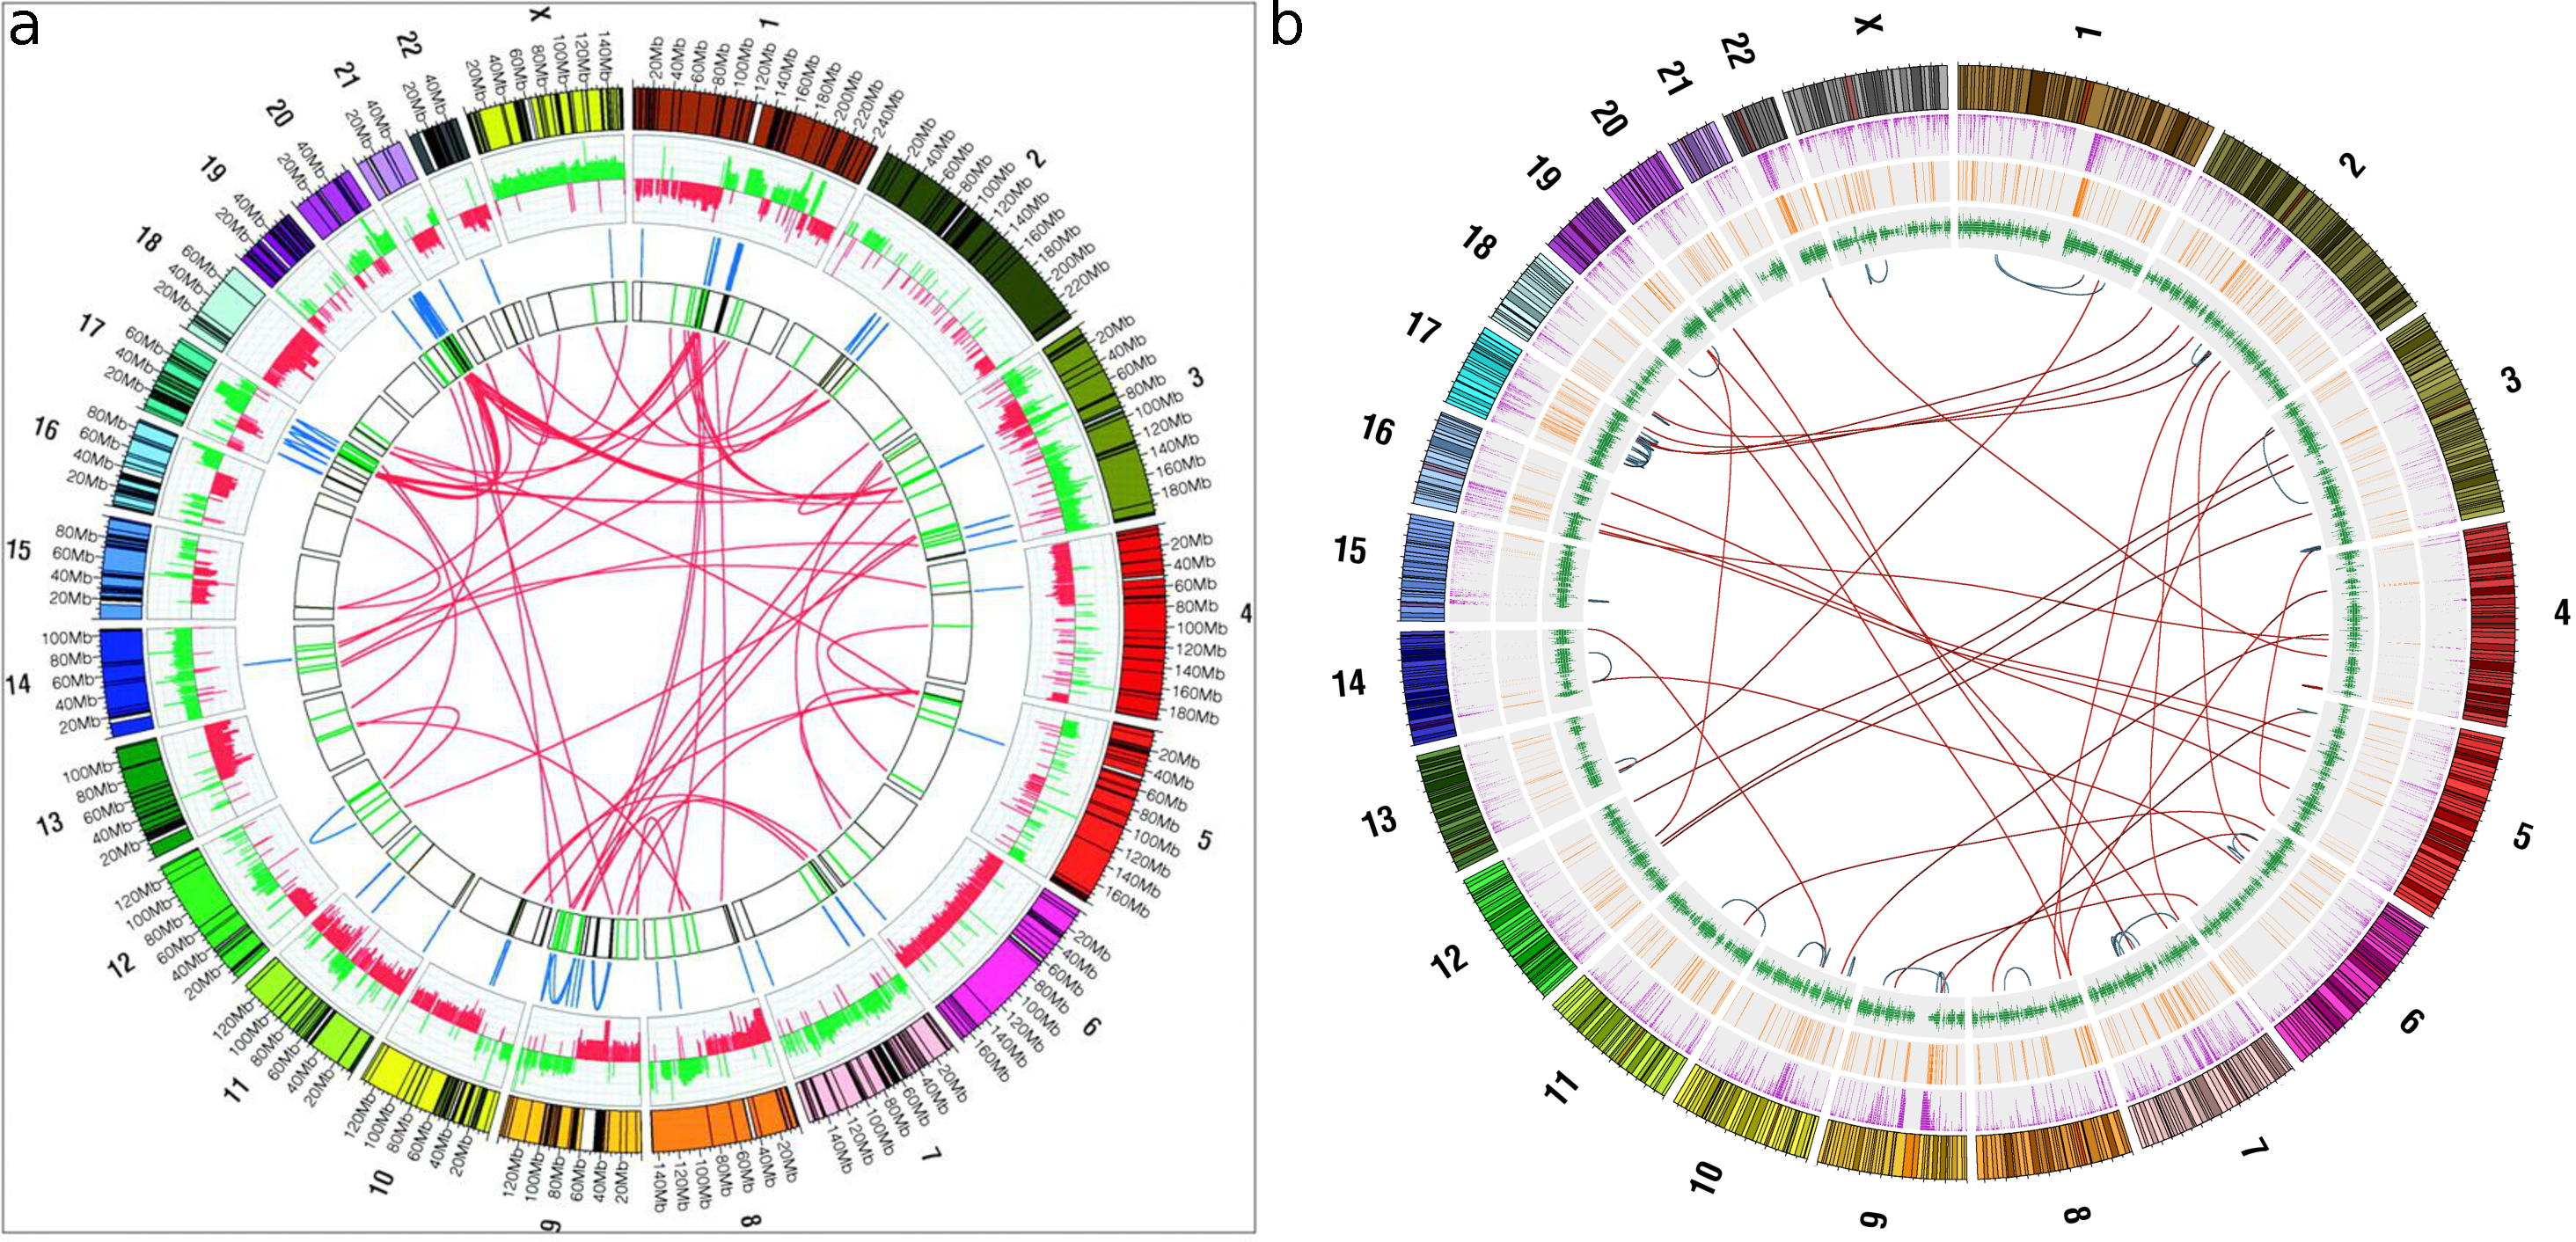
\includegraphics[width=.9\textwidth]{figures/breakpoints_in_cancer_and_evolution.pdf}
\caption{Similarity of genomic breakpoints that occur in cancer and evolution. The regions around the circle represent the human chromosomes. Lines in the centers of the circles show rearrangements between and within chromosomes. A) Somatic rearrangements detected within a breast cancer cell line, adapted from~\cite{Hampton:2009fc}. B) Rearrangements with respect to the human genome sequence present in the gibbon genome, adapted from~\cite{Carbone:2009p1012}.}
\label{cancer_evolution_breakpoints}
\end{figure}

The current technology to detect genomic variations is massively parallel, high-throughput sequencing. This procedure involves amplifying the DNA from a sample and then shearing it into small fragments. The ends of those fragments are then sequenced, producing hundreds of millions or billions of \emph{read pairs} for a sample using current, widely used instruments. The challenge of genomics is then to discover the variants present in the sample using only these short reads. By generating and sequencing enough fragments from a sample (quantified in terms of \emph{coverage}, the average number of reads that cover any one locus in the reference genome), the hope is that it should be possible to capture almost all of the important variants in a given sample. Current practices suggest that 30X average coverage depth is required to achieve accuracy in detecting SNVs. Even with this level of coverage, however, the task is made difficult by errors in the sequencing process, the fact that mammalian genomes are filled with repetitive sequences that make it difficult to ascertain the location in the genome that generated a particular read pair, and the computational challenges of analyzing the volume of data generated.

While SNVs and indels can be characterized relatively well from sequencing data using current algorithmic approaches, the identification of SVs remains challenging. SVs often arise within repetitive regions of the genome, making it difficult to align the reads surrounding them unambiguously to the reference genome. In addition, when the boundaries of an SV (the \emph{breakpoints}) fall within a read sequence, it can be difficult to map that read back to its point of origin in the reference sequence. Although some approaches are based on searching for reads that contain breakpoints, it is often necessary to fall back on other signals present in the read set: the distance between successfully mapped read pairs, which should match the size of the fragments generated in the sequencing protocol, and the depth of reads that cover individual loci along the genome. Detection of SVs with current high-throughput sequencing technology remains a difficult problem, with limited concordance between available algorithms and high false discovery rates~\cite{Mills:2011p1611}.

While current approaches struggle with accuracy, they also often fail to consider speed and scalability. A 30X coverage data set for an individual sample, in compressed format with associated quality scores, is over 100GB of data to analyze. A typical bioinformatic pipeline includes steps to run quality control checks on the raw data; align the reads to the reference genome; perform filtering and recalibration steps after alignment; call SNVs and indels; and finally search for SVs. While a great deal of effort has been put into developing, optimizing, and parallelizing fast methods for alignment and variant calling, SV detection algorithms have not received the same attention, primarily because research in SV detection algorithms has focused on improving accuracy. As large scale sequencing projects like the 1000 Genomes Project and The Cancer Genome Atlas grow, the need for fast and accurate algorithms is becoming more apparent. DNA sequencing is already moving into the clinic, which will only exacerbate this requirement by requiring rapid analysis turnarounds for patients.

One approach to scaling data analysis pipelines is to harness the power of distributed computing using frameworks that tie together clusters of servers. Google's MapReduce~\cite{Dean:2008p277} framework was designed to manage the storage and efficient processing of very large scale data sets across clusters of commodity servers. Hadoop is an open source project of the Apache Foundation which provides an implementation of the MapReduce programming framework as well as a distributed file system (HDFS) for distributing the redundant storage of large data sets across a cluster. Hadoop/MapReduce are rapidly becoming a standard in industrial data mining applications. However, it requires the use of a specific programming model, which can make it difficult to design general-purpose algorithms for arbitrary sequencing analysis problems like SV detection. 

This thesis presents several novel techniques for detecting SVs using distributed computing and machine learning, which derive from the development of an algorithmic framework for SV detection methods in MapReduce. In particular, the main contributions are:

\begin{itemize}
 \item The description of an algorithmic framework for solving SV detection problems in Hadoop and MapReduce based on the computation of local features along the genome from paired end mappings (Chapter~\ref{chap_framework}).
 \item The development in this framework of a software package, Cloudbreak, for discovering genomic deletions up to 25,000bp long, and short insertions, which improves accuracy over existing approaches and uses distributed computing to achieve dramatically faster runtimes (Chapter~\ref{chap_cloudbreak_impl} and Chapter~\ref{chap_cloudbreak_eval}).
 \item An evaluation of the strengths and weaknesses of Cloudbreak when tested on several real and simulated data sets (Chapter~\ref{chap_cloudbreak_eval}).
 \item An exploration of the use of local features as described in Chapter~\ref{chap_framework} to reformulate SV detection as a sequence labeling problem, and the corresponding implementation and evaluation of a conditional random field model to create a novel method for integrating different signals of structural variations (Chapter~\ref{chap_crf}).
\end{itemize}

In separate work not related to the algorithmic developments listed above, we also present the results of data analysis projects which examined the SVs that have massively rearranged the genome of the gibbon in an evolutionary time frame. This has led to the additional contribution of:

\begin{itemize}
 \item Identification of sets of genomic features that are enriched near the breakpoints of the structural variations are present between gibbons and humans. These include segmental duplications and some families of transposable elements, as well as evolutionarily shared transcription factor binding sites. This analysis enhances our understanding of gibbon genome rearrangements. (Chapter~\ref{chap_breakpoint_analysis}).
\end{itemize}

A preliminary version of parts of this work was peer-reviewed and accepted for oral presentation at the Third Annual RECOMB Satellite Workshop On Massively Parallel Sequencing (RECOMB-seq). A preliminary breakpoint analysis was published in~\cite{Capozzi:2012bb}. Throughout this document, I have tried to explicitly identify any work that was carried out by my collaborators.

\chapter{Introduction}

Every normal cell of every human being contains two sets of 23 chromosomes, with the chromosomes in each set holding approximately three billion chained nucleotides of DNA. This DNA contains the instructions that the cell uses to code for the proteins that ultimately specify the behavior of the cell, and in aggregate affect the characteristics of the individual to whom the cell belongs. The differences between the DNA of the cells in two individuals can explain differences in their physical characteristics, their risk of disease, and their population origin and evolutionary history. If one of the cells is cancerous, the differences in the DNA of two cells in one individual can explain the origin of their disease and potentially predict effective treatments.

The aim of the field of \emph{genomics} is to understand the structure and function of the DNA of an organism or population of organisms, with the ultimate goal of understanding how the sequence of nucleotides that make up the genome affect the phenotypes of individuals. To do so, it is necessary to identify and understand all of the differences between the DNA from two samples, whether the samples come from two different individuals or two different tissues from the same individual. If the species has been widely studied, a \emph{reference genome} is often used in place of one of the samples. This allows variations between individuals to be canonically described as variations between the sample and the reference. Experiments of this type are known as \emph{resequencing} experiments.

Assuming that a reference is used, or that the samples come from an individual or individuals from the same or closely related species, the majority of the DNA sequence will be the same between the two samples. In that case, variants can be categorized into one of several forms. The first is a difference of a single base of DNA at a particular location within the genome, or a single nucleotide variant (SNV). If the variation is shared between many individuals in a population, these are referred to as single nucleotide polymorphisms (SNPs). Another type of variation is the insertion or deletion of a small number of base pairs at a particular location, commonly referred to as \emph{indels}. A final category of variants are genomic \emph{structural variations} (SVs). This term describes variations that affect a large number of bases of DNA (in common usage at least 40 base pairs, ranging up to hundreds of megabases or entire chromosomes). SVs can take a variety of forms: strings of DNA can be deleted, inserted, duplicated, inverted, or translocated to a different chromosome. Because they can be large and frequent, SVs account for the majority of the bases that differ among normal human genomes~\cite{Mills:2011p1611, Conrad:2010ja}.

All of these types of variants can alter the function of a genome in different ways. SNVs can change the sequence of the proteins coded for by genes, sometimes altering their function and sometimes rendering them inactive, or they can alter regulatory elements and cause genes to be expressed at differing levels. Indels typically disrupt the function of a gene or regulatory element. SV's can cause a variety of functional changes, ranging from the deletion of exons to the formation of fusion genes such as the famous Brc-Abl Philadelphia chromosome in chronic myelogenous leukemia~\cite{Kurzrock:2003bz}. 

In fact, SV's are very common in some types of cancer, producing extremely rearranged genomes. Because of this, they have particular importance in cancer research, and it is therefore essential to be able to identify them in biological samples, as well as to characterize their functional impact and the mechanisms of their formation. The SV's that arise in cancer genomes have similarities to those that have arisen between different species in evolution (Figure~\ref{cancer_evolution_breakpoints}). For example, the genomes of gibbon species, while still closely related to humans and other apes, have undergone a variety of chromosomal rearrangements and other structural variations when compared to these other species; many more, in fact, than are typical in species with similar levels of divergence. Understanding the evolutionary changes in gibbons, therefore, may shed light on the much faster processes that take place in progenitor cancer cells.

\begin{figure}
\centering
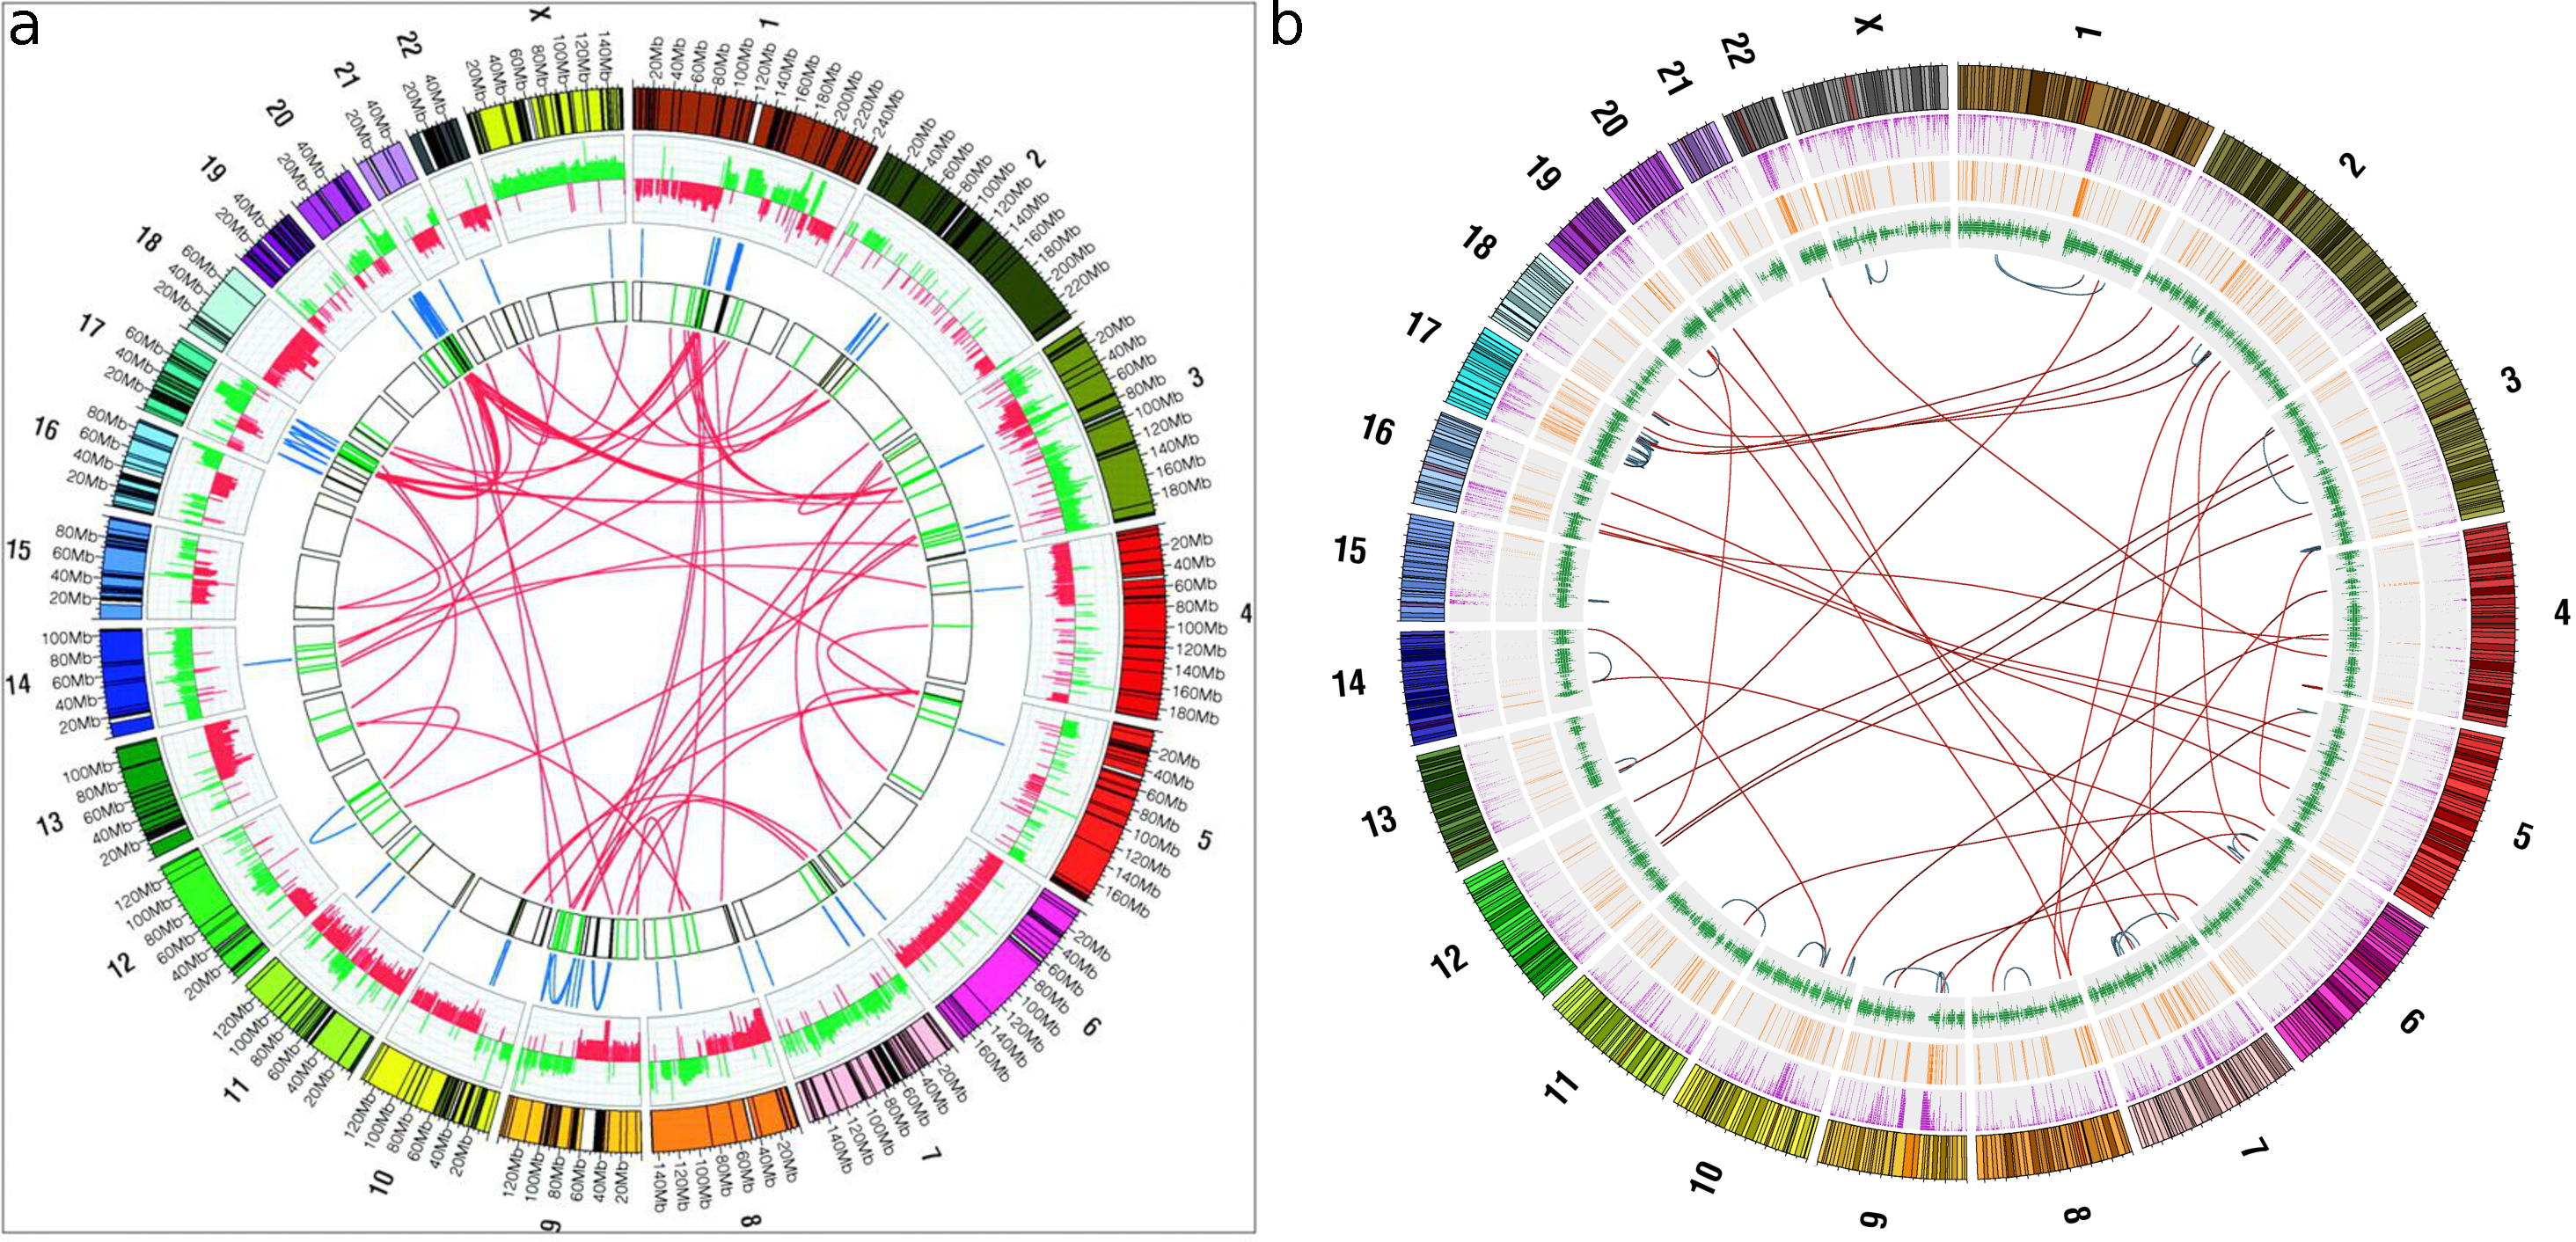
\includegraphics[width=.9\textwidth]{figures/breakpoints_in_cancer_and_evolution.pdf}
\caption{Similarity of genomic breakpoints that occur in cancer and evolution. The regions around the circle represent the human chromosomes. Lines in the centers of the circles show rearrangements between and within chromosomes. A) Somatic rearrangements detected within a breast cancer cell line, adapted from~\cite{Hampton:2009fc}. B) Rearrangements with respect to the human genome sequence present in the gibbon genome, adapted from~\cite{Carbone:2009p1012}.}
\label{cancer_evolution_breakpoints}
\end{figure}

The current technology to detect genomic variations is massively parallel, high-throughput sequencing. This procedure involves amplifying the DNA from a sample and then shearing it into of small fragments. The ends of those fragments are then sequenced, producing hundreds of millions or billions of \emph{read pairs} for a sample using current, widely used instruments. The challenge of genomics is then to discover the variants present in the sample using only these short reads. By generating and sequencing enough fragments from a sample (quantified in terms of \emph{coverage}, the average number of reads that cover any one locus in the reference genome), the hope is that it should be possible to capture almost all of the important variants in a given sample. Current practices suggest that 30X average coverage depth is required to achieve accuracy in detecting SNVs. Even with this level of coverage, however, the task is made difficult by errors in the sequencing process, the fact that mammalian genomes are filled with repetitive sequences that make it difficult to ascertain the location in the genome that generated a particular read pair, and the computational challenges of analyzing the volume of data generated.

While SNVs and indels can be characterized relatively well from sequencing data using current algorithmic approaches, the identification of SV's remains challenging. When the boundaries of an SV (the \emph{breakpoints}) fall within a read sequence, it can be difficult to map that read back to its point of origin in the reference sequence. In addition, SVs often arise within repetitive regions of the genome, further complicating the mapping effort. Although some approaches are based on searching for reads that contain breakpoints, it is often necessary to fall back on other signals present in the read set: the distance between successfully mapped read pairs, which should match the size of the fragments generated in the sequencing protocol, and the depth of reads that cover individual loci along the genome. Detection of SVs with current high-throughput sequencing technology remains a difficult problem, with limited concordance between available algorithms and high false discovery rates~\cite{Mills:2011p1611}.

While current approaches struggle with accuracy, they also often fail to consider speed and scalability. A 30X coverage data set for an individual sample, in compressed format with associated quality scores, is over 100GB of data to analyze. A typical bioinformatic pipeline includes steps to run quality control checks on the raw data; align the reads to the reference genome; perform filtering and recalibration steps after alignment; call SNVs and indels; and finally search for SVs. While a great deal of effort has been put into developing, optimizing, and parallelizing fast methods for alignment and variant calling, SV detection algorithms have not received the same attention, primarily because research in SV detection algorithms has focused on improving accuracy. As large scale sequencing projects like the 1000 Genomes Project and The Cancer Genome Atlas grow, the need for fast and accurate algorithms is becoming more apparent. DNA sequencing is already moving into the clinic, which will only exacerbate this requirement by requiring rapid analysis turnarounds for patients.

One approach to scaling data analysis pipelines is to harness the power of distributed computing using frameworks that tie together clusters of servers. Google's MapReduce~\cite{Dean:2008p277} framework was designed to manage the storage and efficient processing of very large scale data sets across clusters of commodity servers. Hadoop is an open source project of the Apache Foundation which provides an implementation of the MapReduce programming framework as well as a distributed file system (HDFS) for distributing the redundant storage of large data sets across a cluster. Hadoop/MapReduce are rapidly becoming a standard in industrial data mining applications. However, it requires the use of a specific programming model, which can make it difficult to design general-purpose algorithms for arbitrary sequencing analysis problems like SV detection. 

With this in mind, I have developed and evaluated methods for SV detection in the MapReduce framework. In addition, I have used distributed computing to aid in the analysis of genomic DNA breakpoints. I will describe this work and its extensions in my thesis, which will contain the following contributions:

\begin{itemize}
 \item The description of a framework for solving SV detection problems in Hadoop and MapReduce based on the computation of local features along the genome from paired end mappings.
 \item The development in this framework of a software package, Cloudbreak, for discovering genomic deletions up to 25,000bp long, and short insertions, which improves accuracy over existing approaches and uses distributed computing to achieve dramatically faster runtimes.
 \item The analysis of several cancer sequencing data sets using Cloudbreak and other existing SV detection tools, including the development of a pipeline for prioritizing high quality candidate SVs.
 \item An extension of Cloudbreak to incorporate machine learning techniques to further improve SV detection accuracy.
 \item The analysis of sets of genomic breakpoints from cancer and evolutionary data sets. I will examine a set of evolutionary breakpoints discovered in the gibbon genome, and sets of somatic breakpoints discovered in cancer samples. The analysis will search for genomic features that are associated with breakpoints to determine either correlative or causative factors associated with breakpoint formation and preservation.
\end{itemize}

A preliminary version of parts of this work was peer-reviewed and accepted for oral presentation at the Third Annual RECOMB Satellite Workshop On Massively Parallel Sequencing (RECOMB-seq), and an expanded version of that paper is in the process of being submitted for journal publication. A preliminary breakpoint analysis was published in~\cite{Capozzi:2012bb}.

\chapter{Background}

\section{Structural Variations}

\section{High-Throughput Short-Read Sequencing}

\section{Sequencing Analysis Pipelines}

% \input{related-work}
\chapter{Related Work}

\section{Structural Variant Calling from High-Throughput Short-Read Sequencing Data}

Recent publications have divided the majority of popular SV detection algorithms into four categories~\cite{Alkan:2011p547}. The first three categories depend upon first aligning short reads to the reference genome. Read pair (RP) based methods use the distance between and orientation of the mappings of the sequenced ends of DNA fragments to identify the signatures of SVs. Read depth (RD) approaches identify regions of the genome with anomalous raw numbers of mapped reads, which may indicate the presence of deletions or duplications (a category of SV's known as \emph{Copy Number Variations} (CNVs)). Split Read (SR) approaches attempt to find local mappings of portions of individual reads that span SV breakpoints. Finally, assembly-based methods attempt to construct as much of the genome sequence as possible directly from the reads, without first mapping them to the reference genome. The constructed sequence is then compared to the reference to identify SVs. Beyond these four categories, several recent approaches have attempted to integrate more than one type of signal to increase accuracy.

\subsection{Read Pair Approaches}

Most read pair approaches begin by separating paired end mappings onto the reference genome into those that are \emph{concordant} and those that are \emph{discordant}. Discordant mappings deviate from the expected insert size or orientation of the fragment. These approaches then cluster the discordant mappings to find SVs with support from multiple discordantly mapped read pairs. Many of these approaches use only reads that are unambiguously mapped to the reference genome; this has the advantage of using the same set of alignments that are used for calling SNVs and indels in most sequencing pipelines. The BreakDancerMax component of BreakDancer~\cite{Chen:2009p3} is probably the most widely used of these algorithms. BreakDancer looks for regions of the genome that anchor more anomalous read pairs than expected according to its model; if two of these regions are connected by a minimum number of discordant read pairs, it calls an SV that links them. GASV~\cite{Sindi:2009gu}, PEMer~\cite{Korbel:2009dy}, and SVDetect~\cite{Zeitouni:2010p8} all operate on similar principles, differing primarily in the method used to cluster discordant read pairs that support the same potential SV call.

A second group of RP methods attempt to including discordant read pairs which cannot be unambiguously mapped to the reference genome in their analysis, in an attempt to improve sensitivity in repetitive regions of the genome. One approach to incorporating this type of information can be found in \emph{soft clustering} algorithms, which attempt to assign each ambiguously mapped read pair to one of its mappings such that it clusters with other discordant read pairs. These approaches include VariationHunter~\cite{Hormozdiari:2009p284}, which attempts to assign reads by optimizing to a maximum parsimony explanation of all discordant reads; HYDRA~\cite{Quinlan:2010gf}, which takes a similar approach based on heuristics, and GASVPro~\cite{Sindi:2012kk}, which uses a Markov-Chain Monte Carlo sampling strategy to assign a read to its correct mapping. Even so, however, most methods use only a limited number of ambiguous discordant mappings per read pair, in part because of the storage and computational requirements necessary to process all or most ambiguous mappings of each read pair in a high-coverage data set.

Finally, CLEVER~\cite{Marschall:2012ek} took an alternative approach and showed that rather than classifying pairs as concordant or discordant and considering only those that are discordant, considering the distribution of all insert sizes allows the detection of smaller events. 

Read pair approaches have the advantage of being theoretically able to detect any type of SV except for multiple copy number duplications. Their disadvantages stem from the fact that they depend on comparing mapping distances between reads to the unknown size of the fragments from which they came. This means that they cannot capture the breakpoints of SVs with single nucleotide resolution, and that they depend on having a sequencing library with a tight distribution of fragment sizes in order to have power.

\subsection{Read Depth Approaches}

Read-depth (RD) approaches consider the changing depth of coverage of concordantly mapped reads along the genome to infer the presence of SVs. For example, a homozygously deleted region will have zero coverage in the reference genome, while a region that has been duplicated many times, as can happen in some regions of the genome and in some cancers, will have a much higher coverage than average. These approaches differ mainly in the statistical and signal processing techniques used to identify anomalous regions. For example, CNVnator~\cite{Abyzov:2011bk} uses a mean-shift approach to segment the genome into CNV regions. Other approaches in this category include MrFAST~\cite{Alkan:2009cr}, Event-Wise Testing~\cite{Yoon:2009kb}, and SegSeq~\cite{Chiang:2009di}.

RD approaches are good at finding large deletions and duplications. As previously noted, they are the only approach that can identify segments of the genome that have been duplicated multiple times. Their disadvantages are their lack of ability to reliably detect smaller events, and their breakpoint resolution, which is even lower than than of RP approaches.

\subsection{Split Read Approaches}

Split-read (SR) methods look for breakpoints within individual reads by mapping portions of the read to different genomic locations. Due to the computational challenge involved in aligning reads to the reference genome while allowing for very large gaps between portions of the read, they use different strategies to guide the search. Pindel~\cite{Ye:2009p2} looks for paired reads in which one read in the pair aligned to the reference genome but the other did not. Supposing that the other read may contain a breakpoint, it searches the reference nearby for split read mappings. CREST~\cite{Wang:2011p1607} takes advantage of aligners that insert gaps at the ends of read alignments when there are many mismatches between the read and the reference, known as \emph{soft clipping}. By looking for multiple alignments with soft clips at the same reference coordinate, it can identify breakpoints. 

Split read approaches can identify SVs with high specificity and single base breakpoint accuracy. They are particularly good at detecting smaller variants. However, their sensitivity is limited by coverage and the length of the reads. As read lengths increase with advances in sequencing technology, they will play a larger role in SV detection.

\subsection{Assembly-Based Approaches}

An alternative approach to mapping reads to the species reference to discover variants is to first attempt to directly assemble the genomic sequence from which the reads were generated (AS approaches). This typically involves the construction of a \emph{de Bruijn} graph to represent the overlapping k-mers in the entire read set, and then walking the graph to construct the longest possible unambiguous sequence of k-mers. Although most work in assembly is focused on \emph{de novo} assembly, when there is no reference for the organism being sequenced, one approach that is targeted at detecting SV's, among other goals, is Cortex~\cite{Iqbal:2012p1837}. Cortex uses the reference to guide assembly with a colored de Bruijn graph structure, and can therefore identify SVs by walking colored paths in its graph.

While AS approaches can theoretically identify any type of SV, in practice assembly requires extremely high coverage (typically 100X). In addition, the computational requirements necessitate high-memory servers, making the task difficult to run on widely available, non-specialized hardware.

\subsection{Hybrid Approaches}

Recently, approaches have started to appear that attempt to combine multiple signals in order to improve accuracy. These fall into two groups: those that attempt to independently execute more than one of the basic approaches described above and then integrate the results, and those that explicitly create new algorithms to process multiple signals simultaneously.

\subsubsection{Pipelines}

Pipelines such as SVMerge~\cite{Wong:2010p1271} and HugeSeq~\cite{Lam:2012jy} independently execute multiple algorithms of different types and then attempt to merge the results together. PeSV-Fisher~\cite{Escaramis:2013dm} implements classical RP and RD approaches and then integrates and filters the results. While the integration of these approaches could detect any type of variant detectable by any individual algorithm, it is difficult to combine results from different approaches in a principled manner, and the large number of dependencies and complex parameterization and configuration required has prevented adoption of these pipelines outside of the laboratories in which they were created.

\subsubsection{Modified Basic Algorithms}

Other tools use one of the four principle approaches outlined above, but have incorporated other signals into their algorithms to improve accuracy. GASVPro~\cite{Sindi:2012kk} is primarily an RP based method, but it used RD signals to validate its predicted breakpoints, assuming that coverage directly around the breakpoint, and in predicted deleted regions, should be reduced. DELLY~\cite{Rausch:2012he} and PRISM~\cite{Jiang:2012cp}, meanwhile, use RP based approaches to identify candidate SV regions, and then guide an SR search for the exact breakpoints of those SVs. Typically, these modifications seem to improve specificity at the expense of sensitivity.

\subsubsection{Mixtures of Distributions}

Another class of hybrid solution explicitly models the expected number of concordant and discordant pairs at normal and variant locations, effectively combining RP and RD strategies. MoDIL~\cite{Lee:2009da} and the BreakDancerMini component of BreakDancer~\cite{Chen:2009p3} model the distribution of insert sizes at candidate locations in the genome using a Gaussian mixture model. This has two advantages: because reads are not categorized as concordant or discordant based on a hard threshold, it is possible to detect smaller insertions and deletions; and these approaches can explicitly model the zygosity (presence of the variant on one or both of the pairs of chromosomes in the cell) of the variant in the sample, and potentially classify the variant as homozygous or heterozygous. The disadvantage of this approach in these implementations has been the computational requirements, although as we shall see, this strategy lends itself to parallelization. SVMiner~\cite{Hayes:2012ia} follows a somewhat similar approach but does not explicitly model the distribution of insert sizes of read pairs; rather, it created feature vectors based on the number of concordant and discordant read pairs at each locus for deletions, or the number of pairs in each orientation for inversions, and fits a mixture model to the observed distribution of feature vectors across all candidate SVs.

\section{Uses of Hadoop/MapReduce in Bioinformatics}

The Hadoop/MapReduce framework has been used for a variety of sequencing-related bioinformatic tasks. A native algorithm for mapping short reads to a reference genome was demonstrated in Cloudburst~\cite{Schatz:2009p278}.However this algorithm fails to scale to large data sets, and since short read mapping is an embarrassingly parallel task, it is easier in practice to distribute chunks of the short reads in a data set to be mapped independently. This approach is taken in Crossbow~\cite{Langmead:2009p1225}, which uses MapReduce tasks to align reads and then call SNPs. Although not implemented in Hadoop, the Genome Analysis Toolkit~\cite{McKenna:2010p1051} implements many sequencing and variant calling functions using a MapReduce model. Other sequencing applications that have been implemented in Hadoop include ChIP-seq peak calling~\cite{Feng:2011p1228}, and computing genome mappability~\cite{Lee:2012bk}. 

To our knowledge, Hadoop/MapReduce have not been used for SV detection, except for the HugeSeq pipeline~\cite{Lam:2012jy}. HugeSeq, however, simply uses Hadoop to execute existing non-Hadoop applications including BreakDancer, Pindel, and CNVnator, so its ability to harness the available computers in a cluster is limited by the capabilities of those algorithms.

\section{Applications of Discriminative Machine Learning to SV Detection}

Another approach to incorporating multiple sequencing signals involves the use of machine learning techniques. forestSV~\cite{Michaelson:2012fj} creates a feature vector at each genomic location that includes information on read depth, the number of discordant pairs, and genome sequence content and annotations. They then trained a random forest classifier to classify regions as normal, deletions or duplications, flanking regions for those types of variants, or potential false positive calls. Similarly, SVM$^2$~\cite{Chiara:2012ey} creates feature vectors for potentially anomalous genomic sites and classifies them with a support vector machine to create insertion and deletion calls.

% \chapter{A Framework for SV Detection in MapReduce}\label{chap_framework}

In the previous two chapters, we discussed the need for scalable approaches to processing high throughput sequencing data, and explored algorithms for detecting genomic structural variations while noting that efficient processing has not been a primary concern in their design. In this chapter we will explore the MapReduce computing paradigm and its open source Hadoop implementation. We will then discuss ways in which Hadoop has been applied to sequencing tasks. Finally, we will describe a general approach for implementing SV detection algorithms in MapReduce and Hadoop, which we will explore in more detail in later chapters.

\section{MapReduce and Hadoop}\label{section_hadoop_description}

MapReduce~\cite{Dean:2008p277} is a parallel computing framework designed at Google to handle computation over very large data sets - in particular, the vast amounts of data produced by Google's web crawlers. These volumes of data are too large to store and access efficiently on single instances or storage arrays, and must therefore be stored in distributed file systems (DFS), in which portions of the data are stored on individual nodes distributed throughout the cluster, rather than on a central file server; MapReduce runs in conjunction with the Google File System (GFS)~\cite{Ghemawat:2003:GFS:945445.945450}. MapReduce was designed to simplify the development of applications that need to process large volumes of that are distributed across large clusters, while hiding the complexity of data and processing distribution and load balancing from the application developer. An overriding goal in its design was to develop a robust framework in scenarios where clusters are composed of hundreds or thousands of commodity machines, which may have high failure rates and heterogeneous performance characteristics. In particular, it is optimized to provide the following benefits automatically to applications built according to its programming model:

\begin{itemize}
\item \textbf{Fault tolerance.} Both data and processing tasks have redundancy built into the application framework due to the expectation of a certain failure rate among the nodes in the cluster. As mentioned earlier, data is distributed over the file system such that individual blocks of data reside on individual nodes in the cluster. Rather than storing single copies of each block, however, the DFS ensures that multiple copies of each block are stored in the file system on different nodes, and if a node fails, will re-replicate blocks to other nodes so that no data is lost. The same philosophy is also applied to the task scheduler/tracker, which breaks up jobs into many small tasks. If the tracker notices an unresponsive task, for example caused by a hardware error on an individual node, it will restart additional tasks to operate on the same input block of data. In this way jobs can continue processing and complete successfully even when worker nodes fail in the middle of their processing.
\item \textbf{Data locality.} Taking note of the fact that the most expensive part of distributed computing is often transferring data over slower network connections, MapReduce makes every effort to schedule tasks on nodes that physically hold a copy of their input data. This philosophy of ``bringing the code to the data'' is key to processing large data sets quickly without saturating cluster networks.
\item \textbf{Scalability.} The framework's goal is allow the size of both the data sets and the cluster to grow seamlessly. As more data is added to a data set, the DFS divides it into blocks and distributes it across available space on the cluster, avoiding bottlenecks in storage capacity, and increasing the number of nodes that have copies of portions of the data set locally. As more nodes are added to the cluster to increase its capacity, they automatically expand the capacity and have data replicated to them. Since tasks are also broken up into small independent pieces, new nodes can also be seamlessly incorporated into the cluster's processing jobs.
\end{itemize}

Clearly, the desirable properties of the DFS are dependent on being able to divide the data into small blocks that can be distributed easily around the cluster. Similarly, the scalability goals for processing depend on dividing up compute jobs into small tasks that can run independently on different cluster nodes. To achieve this, MapReduce requires that developers structure their application into functional components known, unsurprisingly, as \emph{Map} and \emph{Reduce} tasks. This structure is inspired by a functional technique from the Lisp programming language. In functional programming, \texttt{map} is a function that takes a single-argument function $m$ and a list $l$ as arguments and returns a new list which is the result of applying $m$ to every element of $l$. Meanwhile, \texttt{reduce} is a function that takes a binary operator $r$ and a list $l$, and returns the result $r(r(r(l_1,l_2),l_3),...)$, applying $r$ to every element of $l$ and a running result. Many operations can be expressed as an application of \texttt{map} to a list followed by an application of \texttt{reduce}. For example, to find the sum of squares of a list of integers $l$, one would write \texttt{reduce(sum, map(square, $l$)}. Although the semantics of MapReduce's functions are slightly different than those of functional programming~\cite{lammel20081}, its creators hoped to enable the same expressive power while ensuring that applications are decomposed into parallelizable pieces.

In MapReduce, Map tasks are responsible for examining every record in a block of the input set, and emitting information in the form of $\langle key, value \rangle$ pairs. Reduce tasks then take as input all of the values that were emitted by a mapper under a particular key and and produce one or more outputs that summarize or aggregate those values. In order to accomplish the necessary data handling to ensure that reducers receive all of the keys for a particular value, in between the map and reduce phase MapReduce executes a ``shuffle and sort'' procedure, in which each node sorts the output of all of its mappers by key, sends the results for each key to the machine on which the reducer for that key will run, and then on the reduce machine merges the incoming data from map nodes. This distributed sorting phase is often the key to the efficiency and scalability of MapReduce algorithms.

Figure~\ref{mapreduce_example} shows the canonical example MapReduce application. The task is to count the number of occurrences of every word that appears in a large text corpus. In this simple implementation, mappers take as input blocks of the text input. For every word $w$ that they encounter, they emit the key/value pair $\langle w, 1 \rangle$. Reducers then sum all of the values for each word key $w$, which gives the count of occurrences for that word in the input.

\begin{figure}
\centering
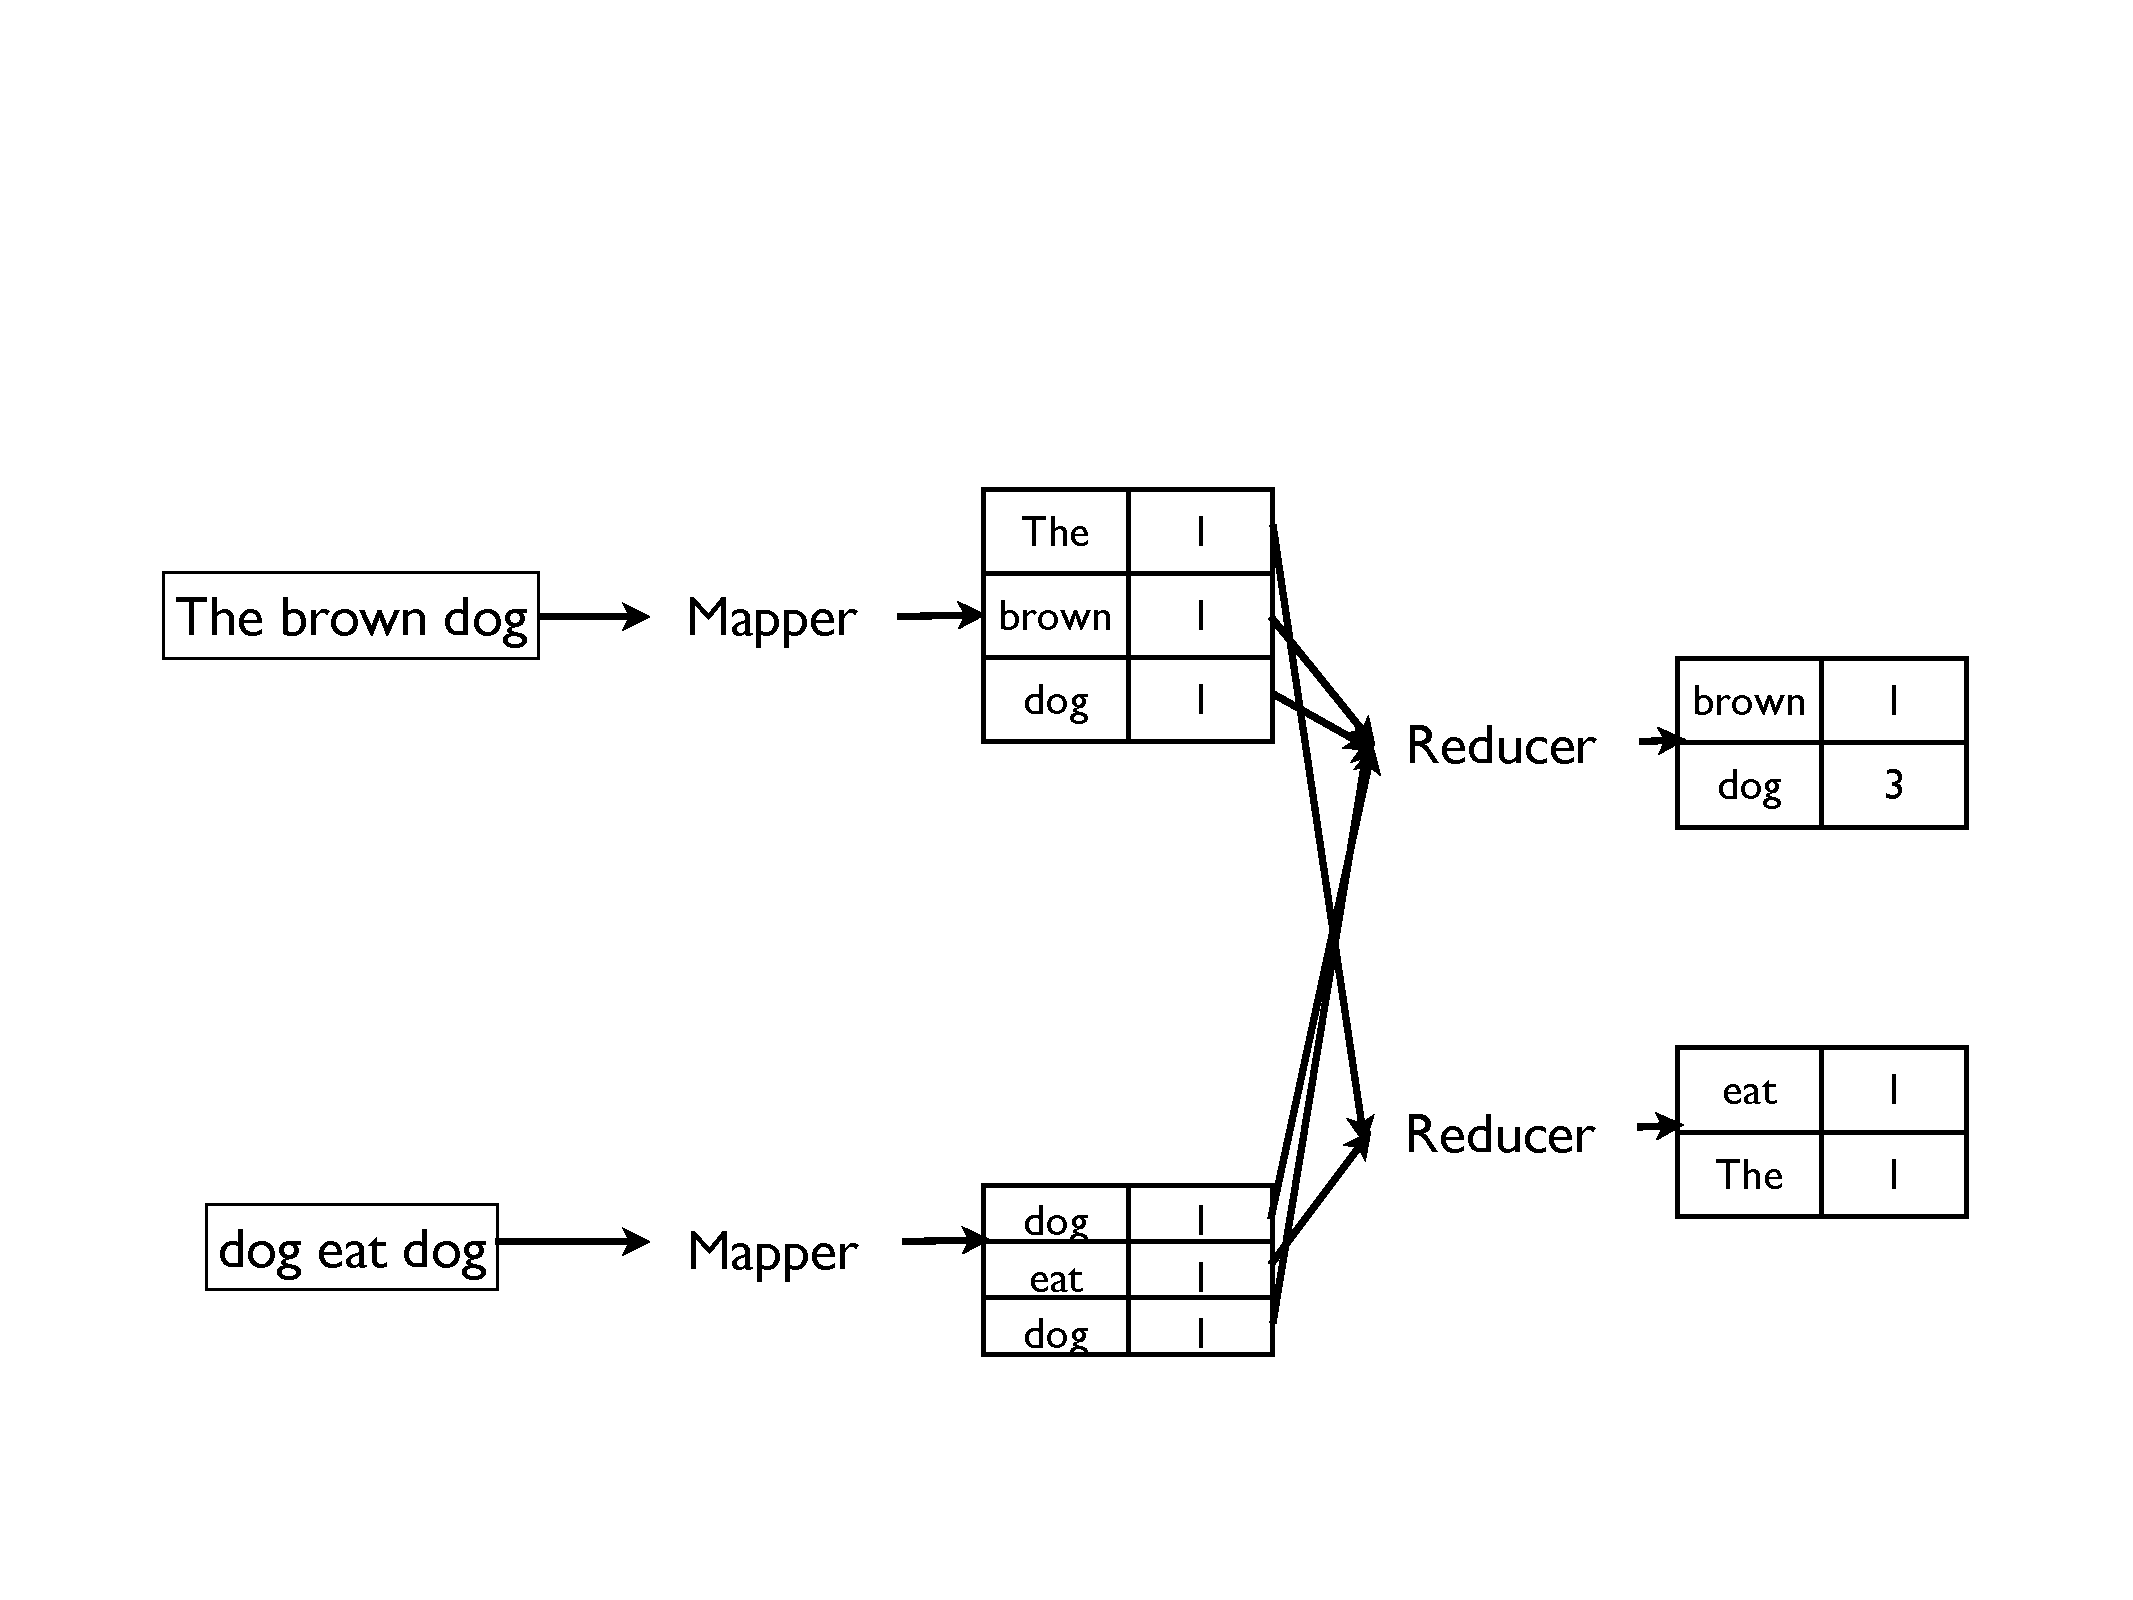
\includegraphics[width=1\textwidth,trim=0in 1in 0in 3in,clip]{figures/mapreduce_example.pdf}
\caption{The word count example MapReduce application. Mappers examine blocks of text data and emit the value one under a key for each word that they encounter. Reducers sum the values they receive for each word, resulting in a count of the number of times each word occurs in the data set.}
\label{mapreduce_example}
\end{figure}

Hadoop is the Apache Software Foundation's open source implementation of the framework described by Google in Dean and Gehemewat's MapReduce paper. It includes an implementation of the MapReduce job scheduler, called the \emph{TaskTracker}, as well as a distributed file system that mimics GFS called HDFS. The open source community has developed Hadoop extensively, with support from many corporations including Yahoo! and Facebook, making it a widely adopted and extended platform for distributed computing.

\section{Uses of Hadoop and MapReduce in Sequencing Tasks}

Now that we understand the components of Hadoop and MapReduce, we can explore its use in sequencing-related bioinformatic tasks. Figure~\ref{bio_hadoop_ecosystem} gives an overview of the published applications of Hadoop to three popular sequencing pipelines: DNA resequencing, RNA-seq, and \emph{de novo} assembly. In some cases, researchers have developed native MapReduce algorithms to solve particular problems. In other instances, Hadoop has been used to run existing tools in parallel; of course, this is only possible when the tasks are embarrassingly parallel at some level. Finally, there are several lower-level APIs, toolkits, and frameworks that have been created in an attempt to ease the development of Hadoop pipelines. These toolkits provide wrappers for reading and writing popular sequencing related file formats, wrappers for commonly used tools, and functions to manipulate short read sequences and alignment records. We will discuss each of these pipelines in more detail in the following sections.

\begin{figure}
\centering
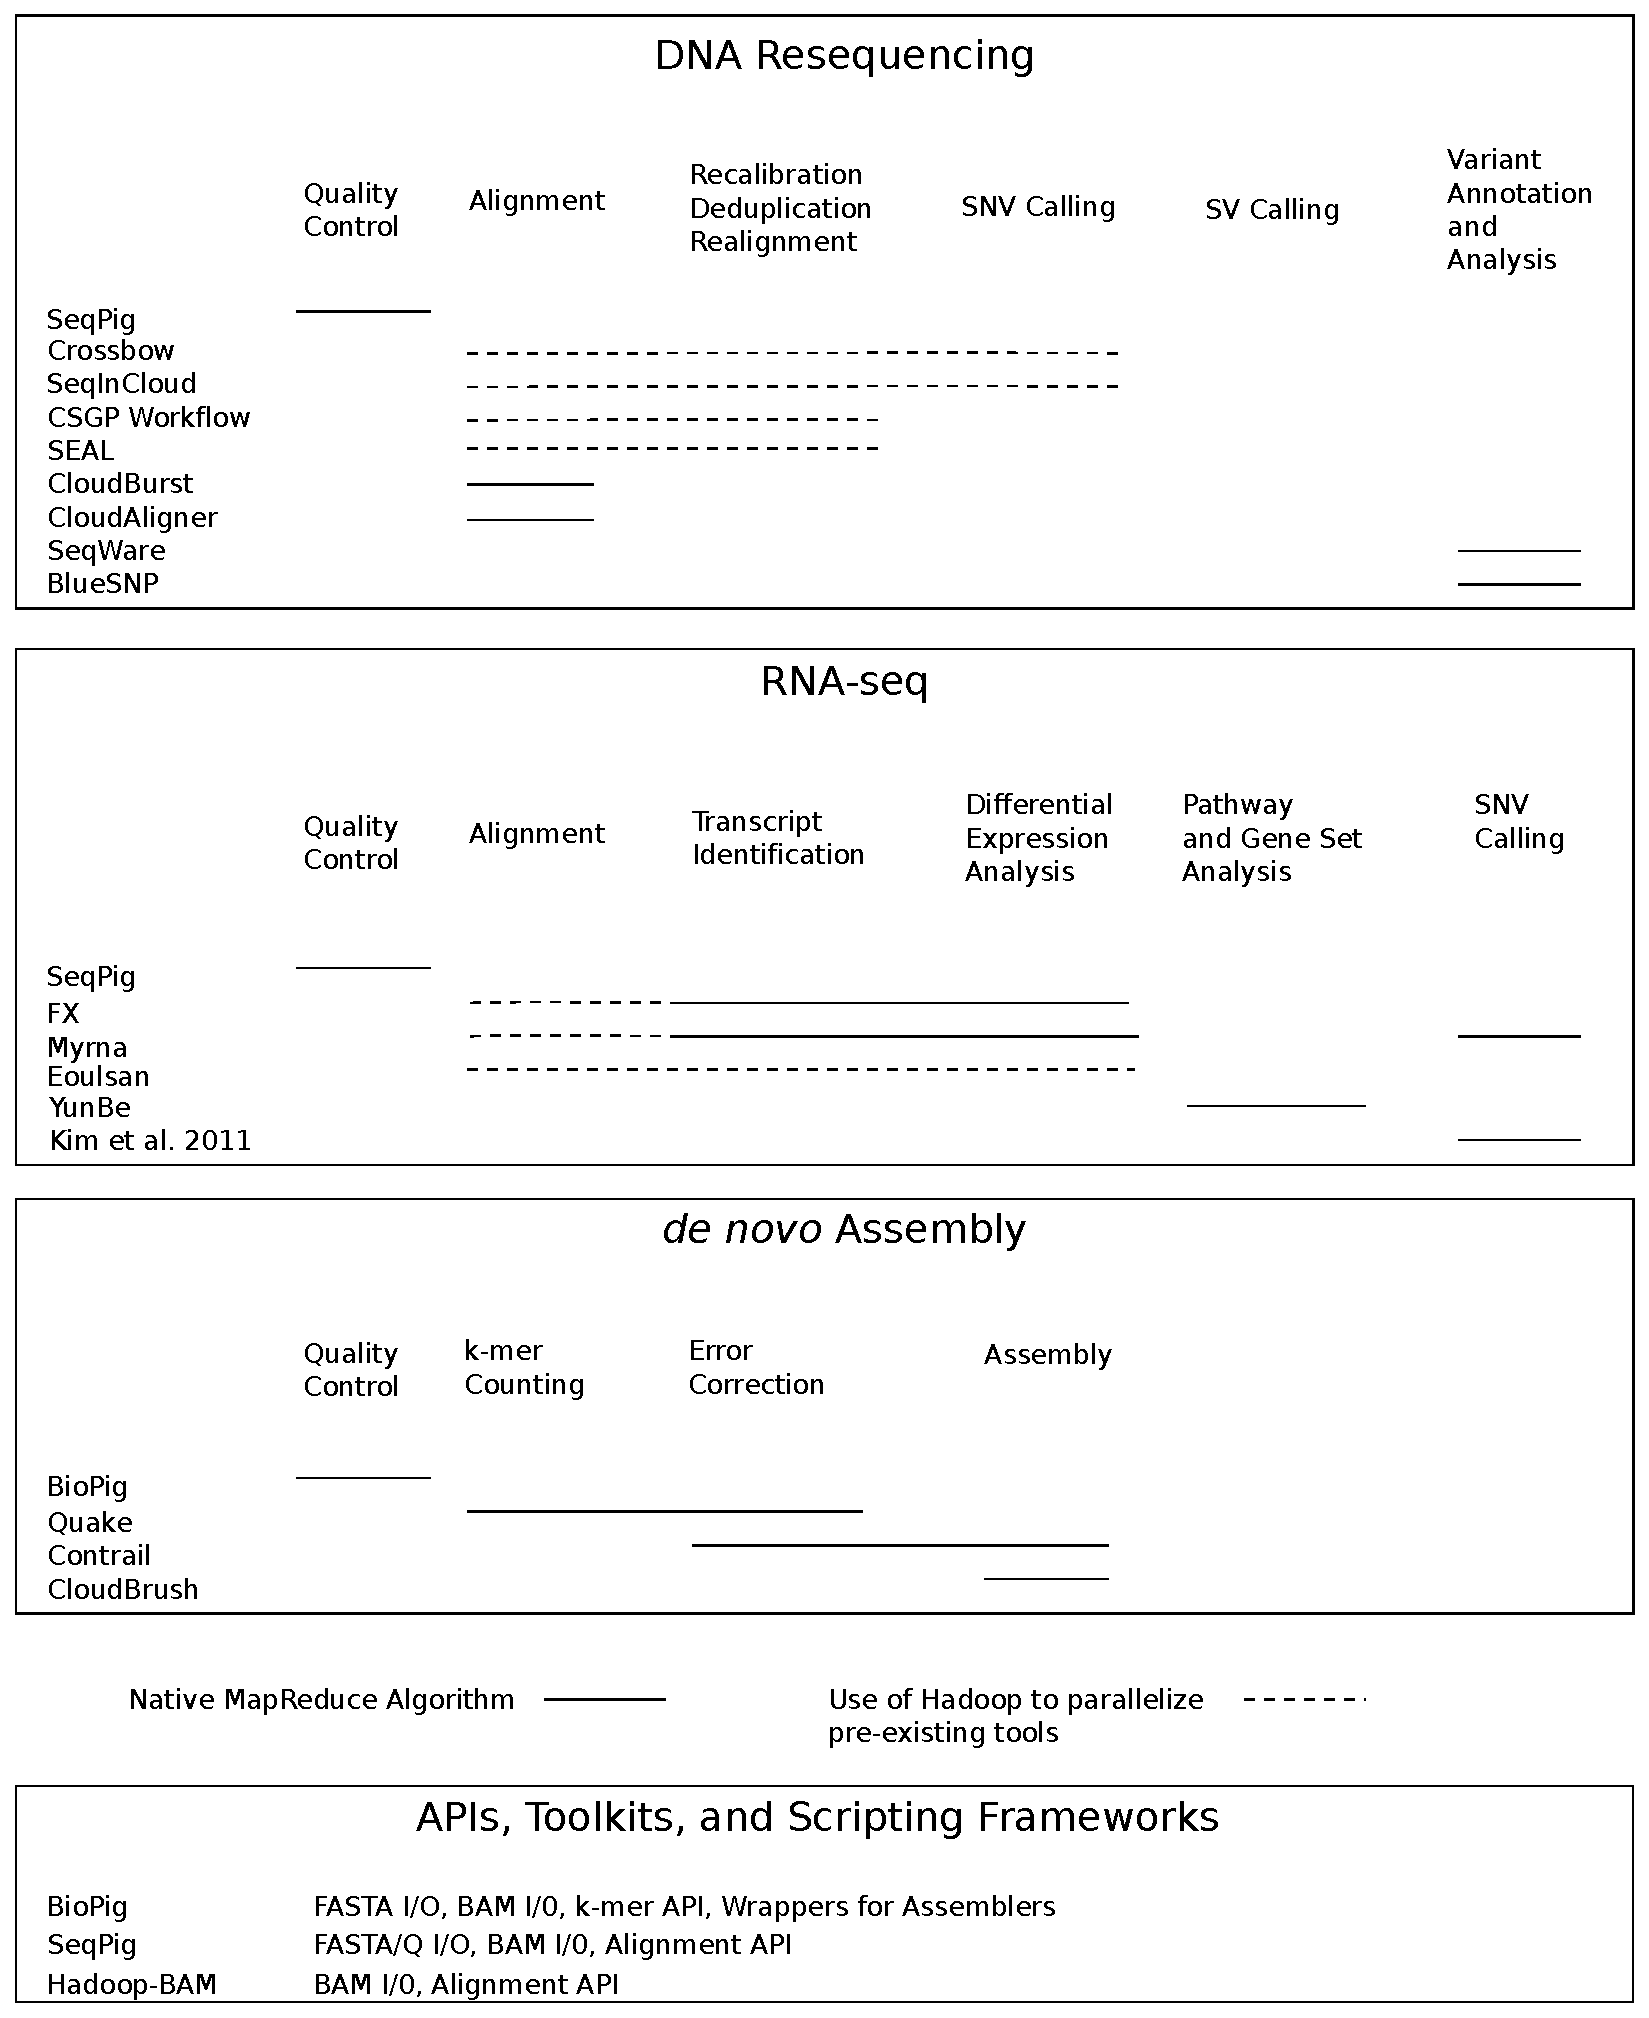
\includegraphics[width=1\textwidth]{figures/bio_hadoop_ecosystem.pdf}
\caption{Hadoop applications to tasks of three popular sequencing analysis pipelines. Solid lines indicate native MapReduce applications developed specifically for Hadoop. Dotted lines indicate pipelines that parallelize the execution of existing tools on splits of the input data using Hadoop. In addition, several toolkits and frameworks are listed that are broadly applicable to many portions of these pipelines.}
\label{bio_hadoop_ecosystem}
\end{figure}

\subsection{DNA Resequencing}

As we discussed in Section~\ref{section_pipelines}, there are multiple steps that are typically part of DNA resequencing pipelines. These steps included quality control analysis, alignment to the genome reference, a series of processes including realignment in problematic regions and removal of duplicate reads, steps to call SNVs and SVs, and finally annotation and analysis of the variants that were discovered. 

A native algorithm for mapping short reads to a reference genome was first demonstrated in Cloudburst~\cite{Schatz:2009p278}. This algorithm creates keys for each k-mer that appears in both the reads and the reference. The reducers then bring together the reads and portions of the reference that match on the same k-mer, and determine whether the match on the seed can be extended to an alignment of the entire read to the reference. Because the read and reference portions are each transferred to the reducers for every single k-mer which appears in them, this algorithm, while accurate, generates large amounts of data that must be shuffled, sorted, and potentially cross the network. Therefore, it is difficult to scale it to very large read sets. This shows the difficulty of designing true MapReduce algorithms that can scale and take advantages of Hadoop's infrastructure. CloudAligner~\cite{Nguyen:2011p1832} uses a similar seed-and-extend algorithm, although the exact details of their map and reduce steps are not specified.

Since short read mapping is an embarrassingly parallel task and highly optimized non-MapReduce alignment tools with full feature sets are readily available, it is more efficient in practice to use the map phase of a Hadoop job to align splits of input reads with existing tools, and then merge results in the reduce phase. SEAL~\cite{Pireddu:2011fj} and the CRS4 Sequencing and Genotyping Platform's CSGP workflow~\cite{Pireddu:2011:MGS:1996092.1996106} are two such pipelines which use the BWA~\cite{Li:2009p836} aligner in each map task. By emitting mappings under a key for the alignment location, they are then able to accomplish the duplicate removal step in the reduce function in a manner similar to that of the popular non-MapReduce tool Picard~\cite{picard}. Similarly, Crossbow~\cite{Langmead:2009p1225} uses Hadoop to parallelize Bowtie~\cite{Langmead:2009p768}. Crossbow then calls single nucleotide variants in the reduce phase using SOAPsnp~\cite{Li:2009p1236}, allowing it to function as a minimum viable pipeline for sequencing. Crossbow also includes infrastructure for running in the Amazon Elastic Compute Cloud, which has contributed to its popularity. SeqInCloud~\cite{nabeel-bicob13-genome-analysis-cloud} similarly combines BWA with the GATK's~\cite{McKenna:2010p1051} realignment and SNV calling steps, along with infrastructure to run in the Microsoft Azure cloud computing platform.

After variant discovery, the usual next step in a resequencing project is to analyze the variants found to detect functional impact (i.e. what genes might be disrupted by the variants found) or to find associations between variants and phenotypes, as in case-control sequencing projects. SeqWare~\cite{Oconnor:2010p1835} uses HBase~\cite{hbase}, a Hadoop database based upon Google's BigTable~\cite{Chang:2008:BDS:1365815.1365816}, to provide functionality to annotate and query the variants. SeqWare uses the genomic coordinates of variants and coverage information as schema keys within HBase's MapReduce queries. BlueSNP~\cite{Huang:2012bb}, meanwhile, implements Hadoop algorithms for finding significant loci and estimating p-values through permutation analysis in genome wide association studies.

To our knowledge, Hadoop/MapReduce have not been used for SV detection. Several non-Hadoop pipelines such as HugeSeq~\cite{Lam:2012jy} and SVMerge~\cite{Wong:2010p1271} use grid scheduling engines like SGE to distribute SV detection tasks across compute clusters. For example, the HugeSeq pipeline is an end-to-end pipeline for DNA resequencing that integrates BreakDancer~\cite{Chen:2009p3}, Pindel~\cite{Ye:2009p2}, CNVnator~\cite{Abyzov:2011bk}, and BreakSeq~\cite{Lam:2010p1383} for SV calling. However, these pipelines can only achieve parallelization by sample or at most by chromosome of the reference, limiting their scalability.

\subsection{RNA-seq}

The goals of RNA-seq are to determine the transcripts and isoforms being expressed, quantify their differential expression, and potentially call DNA variants based on the sequences of the RNA transcripts.  Myrna~\cite{Langmead:2010p1268} and FX~\cite{Hong:2012du} are Hadoop pipelines that execute alignment, transcript identification, and differential expression calculations in multiple Hadoop jobs. Myrna uses Bowtie in each mapper to distribute alignment work across the cluster, and then parallelizes each of the differential expression calculations by first assigning alignments to transcripts, gathering the data by sample to compute normalization factors, and then re-gathering the normalized counts under keys representing transcripts to compute statistics. FX has a less complex workflow, in which alignments are executed in a map-parallel fashion using the GSNAP alignment tool~\cite{Wu:2010p875}, and then has simple steps to count reads by gene for differential expression statistics, and to call SNPs in genes. Both Myrna and FX have infrastructure to automatically create Hadoop clusters in Amazon EC2. Eoulsan~\cite{Jourdren:2012dc} is a very similar workflow, which allows a number of aligners to be used in the mapping step, and then computes read counts per gene in parallel, before computing differential expression statistics outside of the Hadoop environment using existing tools. For use after expression levels have been computed, YunBe~\cite{Zhang:2011p1823} computes statistics to determine whether particular gene pathways have been perturbed in two sets of samples, using a MapReduce strategy where mappers produce expression values from the sample data under keys that represent specific pathways, and reducers aggregate all data for each pathway to determine a ``perturbation statistic'' between sample conditions. Finally, Kim et al.~\cite{Kim2011RNASEQ} described a pipeline for SNV detection from RNA-seq data based on a Hadoop job in which the mappers emit each base and quality score from the aligned reads under a key representing the genomic coordinate, and reducers call the absence or presence of a SNV at each location.

\subsection{\emph{de novo} Assembly}

The third major pipeline for which there has been significant interest in applying Hadoop and MapReduce is \emph{de novo} assembly. Most state-of-the-art algorithms for assembly depend on building large data structures that model the overlaps between reads (in the case of string graph based approaches) or between k-mers found in the reads (in the case of de Bruijn-graph algorithms) as edges in a graph. Given the high depth of coverage that is needed to produce a quality assembly, these graphs become very large, and the need to traverse them requires random rather than sequential access to the data. This would seem to make the problem a poor fit for Hadoop, which is optimized for sequential access of large data sets on commodity hardware. Nevertheless, several groups have attempted to create assembly algorithms using MapReduce. Contrail~\cite{schatz2010novo} builds a de Bruijn graph by emitting each pair of consecutive k-mers from the reads as a key-value pair to form a k-mer adjacency matrix. CloudBrush~\cite{Chang:2012hd} uses a ``prefix-and-extend'' strategy~\cite{10.1109/CLOUD.2012.123}, in which all k-mers that appear in the reads are used as keys, with the reads themselves as values. Extension procedures then test whether the k-mer is the prefix of one of the reads and the suffix of another. Both of these tools have then developed MapReduce procedures for graph pruning and traversal that are necessary to produce contigs from their respective graph data structures. Finally, some helpful read pre-processing steps for assembly have been implemented in Hadoop: Quake~\cite{Kelley:2010kg} is a widely used MapReduce k-mer counter, and BioPig~\cite{Nordberg:2013ka} also contains facilities for k-mer analysis of large read sets.

\subsection{Frameworks and Toolkits}

In addition to the pipelines listed above, recently several sequencing-related frameworks and toolkits have been created to ease the development of Hadoop applications. These tools include APIs and library code to handle reading from and writing to files in popular sequencing data formats. For example, Hadoop-BAM~\cite{Niemenmaa:2012hu} allows manipulation of data in the SAMtools~\cite{Li:2009vz} binary alignment format BAM. Two libraries, SeqPig~\cite{Schumacher:2013kh} and BioPig~\cite{Nordberg:2013ka}, were also recently published that provide file formats and commonly used functions in the Apache Pig~\cite{pig} environment, which provides a high-level programming language called Pig Latin that allows easy expression of simple data analysis tasks. These libraries allow for rapid development of scripts that gather statistics on read and alignment data sets, and Pig automatically optimizes their execution by translating them into one or more MapReduce jobs. 

\subsection{Other uses of Hadoop and MapReduce}

Although not implemented in Hadoop, the very widely used Genome Analysis Toolkit~\cite{McKenna:2010p1051} (GATK) implements many sequencing and variant calling functions using a MapReduce programming model. Although it currently can only distribute tasks across clusters using traditional grid engines, future versions of this package may be re-implemented to use Hadoop. Other notable sequencing applications that have been implemented in Hadoop include ChIP-seq peak calling~\cite{Feng:2011p1228}, and computing genome mappability scores~\cite{Lee:2012bk}. 

\section{MapReduce Constraints on SV Algorithms}

To this point, we know of no Hadoop-based SV detection algorithms. This may be because the need to separate logic into mappers and reducers makes it difficult to implement traditional RP-based SV detection approaches in MapReduce, particularly given the global clustering of paired end mappings at the heart of many RP approaches. MapReduce algorithms, by contrast, excel at conducting many independent calculations in parallel. The sequencing applications that have been implemented in MapReduce succeed by dividing processing into a series of local computation, for example calling a SNV at a particular location in the genome given the reads that cover it, to use the example of Crossbow~\cite{Langmead:2009p1225}, the most widely accepted sequencing MapReduce algorithm. As we noted in Chapter~\ref{chap_related_work}, SV approaches that are similarly based on local computations have been described: the RP-based SV callers MoDIL~\cite{Lee:2009da} and forestSV~\cite{Michaelson:2012fj} try to solve the SV detection problem by computing scores or features along the genome and then producing SV predictions from those features in a post-processing step. In the remainder of this chapter, we formalize this idea and develop it as a potential framework for implementing SV detection algorithms in MapReduce.

\section{A General MapReduce SV Detection Algorithm}\label{section_general_algo}

Using this strategy, we have developed a conceptual algorithmic framework for SV detection in MapReduce, which is outlined in Algorithm~\ref{cb_algo}. This framework divides processing into three separate MapReduce jobs: an alignment job, a feature computation job, and an SV calling job. The overall workflow of the algorithm and its implementation on a compute cluster or cloud is summarized in Figure~\ref{cloudbreak_workflow}.

\begin{figure}
\centering
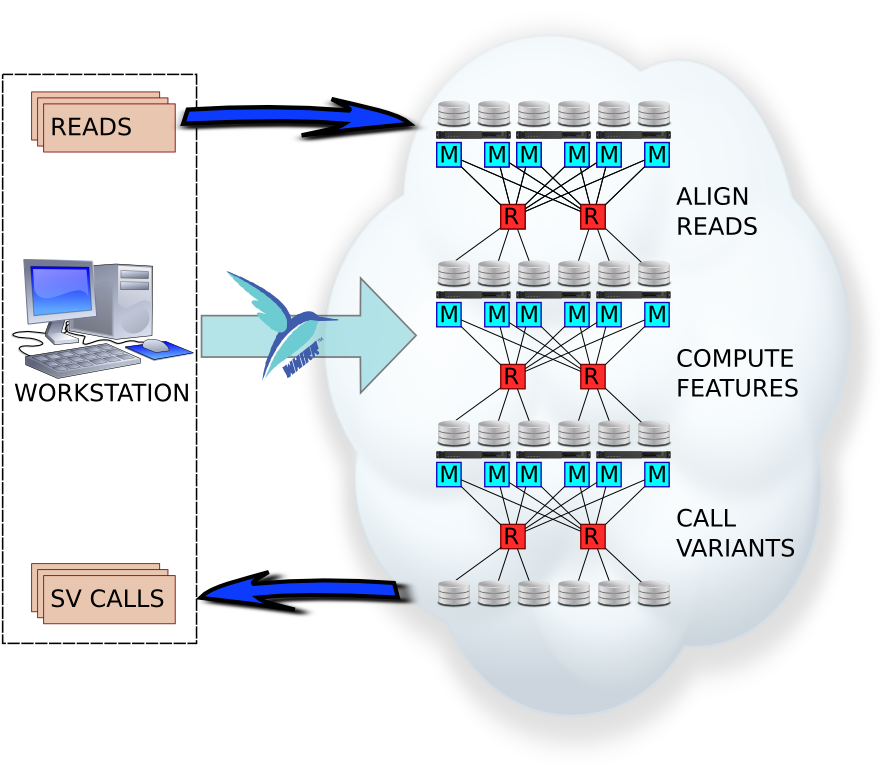
\includegraphics[width=.8\textwidth]{figures/workflow_with_whirr.png}
\caption{An overview of the steps of the MapReduce SV detection workflow. Reads are first uploaded to a Hadoop cluster from local storage. Processing is then then divided into three MapReduce jobs: 1) Mapping with sensitive settings. 2) Computation of features across the genome. 3) Calling structural variations based on the features computed in the previous step. Finally, SV predictions can be downloaded from the Hadoop cluster and examined and annotated. Cloudbreak can also use the Apache Whirr library to automatically provision Hadoop clusters on and deploy data to cloud providers such as Amazon Elastic Compute Cloud.}
\label{cloudbreak_workflow}
\end{figure}


The \textsc{Align Reads} job uses existing alignment tools to discover mapping locations for each read pair. Aligners can be executed to report multiple possible mappings for each read, or only the best possible mapping. Given a set of read pairs, each of which consists of a read pair identifier $rpid$ and two sets of sequence and quality scores $<s,q>$, each mapper aligns each pair end set $<s,q>$ in either single- or paired end mode and emits possible mapping locations under the $rpid$ key. Reducers then collect the alignments for each paired end, making them available under one key for the next job. 

In the \textsc{Compute Features} job, we compute a set of features for each location in the genome. To begin, we tile the genome with small fixed-width, non-overlapping intervals. For the experiments reported in Chapter~\ref{chap_cloudbreak_eval} we use an interval size of 25bp (see Section~\ref{section_window_size} for an exploration of the effects of different window sizes on accuracy and runtime). Let $L = \left\{l_1,l_2,\ldots,l_N\right\}$ be the set of intervals covering the entire genome. Let $R^1 = \left\{r^{1}_{1},r^{1}_{2},\ldots,r^{1}_{M}\right\}$ and $R^2 = \left\{r^{2}_{1},r^{2}_{2},\ldots,r^{2}_{M}\right\}$ be the input set of paired reads. Let $A^1 = \left\{a^{1}_{m,1},a^{1}_{m,2},\ldots,a^{1}_{m,K}\right\}$ and $A^2 = \left\{a^{2}_{m,1},a^{2}_{m,2},\ldots,a^{2}_{m,L}\right\}$ be the set of alignments for the left and right reads from read pair $m$. For any given pair of alignments of the two reads in a read pair, $a^{1}_{m,i}$ and $a^{2}_{m,j}$, let the $\textrm{ReadPairInfo } rpi_{m,i,j}$ be information about the pair relevant to detecting SVs, e.g. the fragment size implied by the alignments and the likelihood that the alignments are correct. We then leave two functions to be implemented depending on the application:
\begin{flalign*}
 \textsc{Loci } :& \langle a^{1}_{m,i},a^{2}_{m,j} \rangle \rightarrow L_m \subseteq L \\
 \Phi :& \left\{\textrm{ReadPairInfo }rpi_{m,i,j}\right\} \rightarrow \mathbb{R}^N \\
\end{flalign*}

The first function, \textsc{Loci}, maps an alignment pair to a set of genomic locations to which it is relevant for SV detection; for example, the set of locations overlapped by the internal insert implied by the read alignments.  We optimize this step by assuming that if there exist concordant mappings for a read pair, defined as those where the two alignments are in the proper orientation and with an insert size within three standard deviations of the expected library insert size, one of them is likely to be correct and therefore we do not consider any discordant alignments of the pair. The second function, $\Phi$, maps a set of ReadPairInfos relevant to a given location to a set of real-valued vectors of features useful for SV detection. 

Finally, the third MapReduce job, \textsc{Call Variants}, is responsible for making SV calls based on the features computed at each genomic location. It calls another application-specific function: 

 \[ \textsc{PostProcess} : \left\{\phi_1,\phi_2,\ldots,\phi_N\right\} \rightarrow \left\{\langle  \textrm{SVType } s, l_{start}, l_{end} \rangle\right\} \]

This function maps the sets of features for related loci into a set of SV calls characterized by their type $s$ (i.e Deletion, Insertion, etc.) and their breakpoint locations $l_{start}$ and $l_{end}$. We parallelize this job in MapReduce by making calls for each chromosome in parallel, which we achieve by associating a location and its set of features to its chromosome in the map phase, and then making SV calls for one chromosome in each reduce task.

\begin{algorithm}
\algrenewcommand\algorithmicprocedure{\textbf{job}}
 \begin{algorithmic}[1]
 \Procedure{Alignment}{}
 \Function{Map}{$\textrm{ReadPairId }rpid, \textrm{ReadId }r, \textrm{ReadSequence }s, \textrm{ReadQuality }q$}
 \ForAll{$ \textrm{Alignments }a \in \textsc{Align}(<s,q>)$}
 \State $\textsc{Emit}(\textrm{ReadPairId }rpid, \textrm{Alignment }a)$
 \EndFor
 \EndFunction
 \Function{Reduce}{$\textrm{ReadPairId }rpid, \textrm{Alignments }a_{1,2,\ldots}$}
 \State $\textrm{AlignmentPairList }ap \gets \textsc{ValidAlignmentPairs}(a_{1,2,\ldots})$
 \State $\textsc{Emit}(\textrm{ReadPairId }rp, \textrm{AlignmentPairList } ap)$
 \EndFunction
 \EndProcedure

 \Procedure{Compute SV Features}{}
 \Function{Map}{$\textrm{ReadPairId }rp, \textrm{AlignmentPairList }ap$}
 \ForAll{$ \textrm{AlignmentPairs }<a_1,a_2> \in ap$}
 \ForAll{$ \textrm{GenomicLocations }l \in \textsc{Loci }(a_1,a_2)$}
 \State $ \textrm{ReadPairInfo }rpi \gets <\textrm{InsertSize}(a_1,a_2), \textrm{AlignmentScore}(a_1,a_2)>$
 \State $\textsc{Emit}(\textrm{GenomicLocation }l, \textrm{ReadPairInfo }rpi)$
 \EndFor
 \EndFor
 \EndFunction
 \Function{Reduce}{$\textrm{GenomicLocation }l, \textrm{ReadPairInfos }rpi_{1,2,\ldots}$}
 \State $\textrm{SVFeatures } \phi_l \gets \Phi(\textrm{InsertSizes }i_{1,2,\ldots}, \textrm{AlignmentScores }q_{1,2,\ldots})$
 \State $\textsc{Emit}(\textrm{GenomicLocation }l, \textrm{SVFeatures } \phi_l)$
 \EndFunction
 \EndProcedure

 \Procedure{Call SVs}{}
 \Function{Map}{$\textrm{GenomicLocation }l, \textrm{SVFeatures } \phi_l$}
 \State $\textsc{Emit}(\textrm{Chromosome}(l), <l,\phi_l>)$
 \EndFunction
 \Function{Reduce}{$\textrm{Chromosome }c, \textrm{GenomicLocation } l_{1,2,\ldots},\phi_{1,2,\ldots}$}
 \State $\textrm{StructuralVariationCalls } svs_c \gets \textsc{PostProcess }(\phi_{1,2,\ldots})$
 \EndFunction
 \EndProcedure
 \end{algorithmic}
\caption{The algorithmic framework for SV calling in MapReduce.}
\label{cb_algo}
\end{algorithm}

\section{Discussion}\label{section_framework_discussion}

The framework that we have just described is agnostic to the type of structural variations that the user wishes to detect. In the next chapter, we describe Cloudbreak, our implementation of this framework that identifies small deletions and insertions. To do so, it defines the relevant information from each pair (the ReadPairInfo) as information about the insert size implied by the mapping of the paired reads, sends them to every location which is spanned by that read pair in the reference genome, and then computes features from them by modeling the expected distribution of insert sizes at each location with a Gaussian Mixture Model. We demonstrate some of the strengths of this particular implementation in Chapter~\ref{chap_cloudbreak_eval}. However, we believe that this general framework could be applied to many other SV detection problems. For example, to detect inversions, one might define a different ReadPairInfo for each pair that includes information about the orientation of the mappings. Translocation detection programs might emit ReadPairInfos that contain information about the chromosomes linked to by interchromosomal mappings, which the $\Phi$ function would then cluster to see if a preponderance of those mappings point to the same breakpoint location. In addition to paired mapping locations, it would also be possible to design ReadPairInfo and feature function definitions that allowed the computation of read depth or split read related features, enabling the integration of more of the signals available in the data set. We will explore one possible way to integrate disparate features such as these in Chapter~\ref{chap_crf}. Use of the Hadoop/MapReduce computing framework would ensure that any of these applications, if carefully designed, could enjoy the benefits of redundancy, data locality, and scalability we described in Section~\ref{section_hadoop_description}, and therefore will be able to grow to meet the rising demands of genomics applications in the near future.

\chapter{A General Framework for SV Detection in MapReduce}

MapReduce~\cite{Dean:2008p277} divides computation across a cluster into three phases. In the first phase, \emph{mappers} developed by the application programmer examine small blocks of data and emit a set of $\langle key, value \rangle$ pairs for each block examined. The MapReduce framework then sorts the output of the mappers by key, and aggregates all values that are associated with each key. Finally, the framework executes \emph{reducers}, also created by the application developer, which process all of the values for a particular key and produce one or more outputs that summarize or aggregate those values. MapReduce and Hadoop allow efficient processing of large data sets by scheduling tasks for execution as close as possible to the nodes which hold the required data, minimizing network traffic and I/O contention.

The need to separate logic into mappers and reducers makes it difficult to implement traditional RP-based SV detection approaches in MapReduce, particularly given the global clustering of paired end mappings at the heart of many RP approaches. MapReduce algorithms, by contrast, excel at conducting many independent calculations in parallel. The sequencing applications that have been implemented in MapReduce succeed by dividing processing into a series of local computation, for example calling a SNV at a particular location in the genome given the reads that cover it, which is the approach taken by the variant callers GATK~\cite{McKenna:2010p1051} and Crossbow~\cite{Langmead:2009p1225}. SV approaches that are similarly based on local computations have been described: the RP-based SV callers MoDIL~\cite{Lee:2009da} and forestSV~\cite{Michaelson:2012fj} attempt to solve the SV detection problem by computing scores or features along the genome and then producing SV predictions from those features in a post-processing step. 

Using this strategy, we have developed a conceptual algorithmic framework for SV detection in MapReduce, which is outlined in Algorithm~\ref{cb_algo}. This framework divides processing into three separate MapReduce jobs: an alignment job, a feature computation job, and an SV calling job. The overall workflow of the algorithm and its implementation on a compute cluster or cloud is summarized in Figure~\ref{cloudbreak_workflow}.

\begin{figure}
\centering
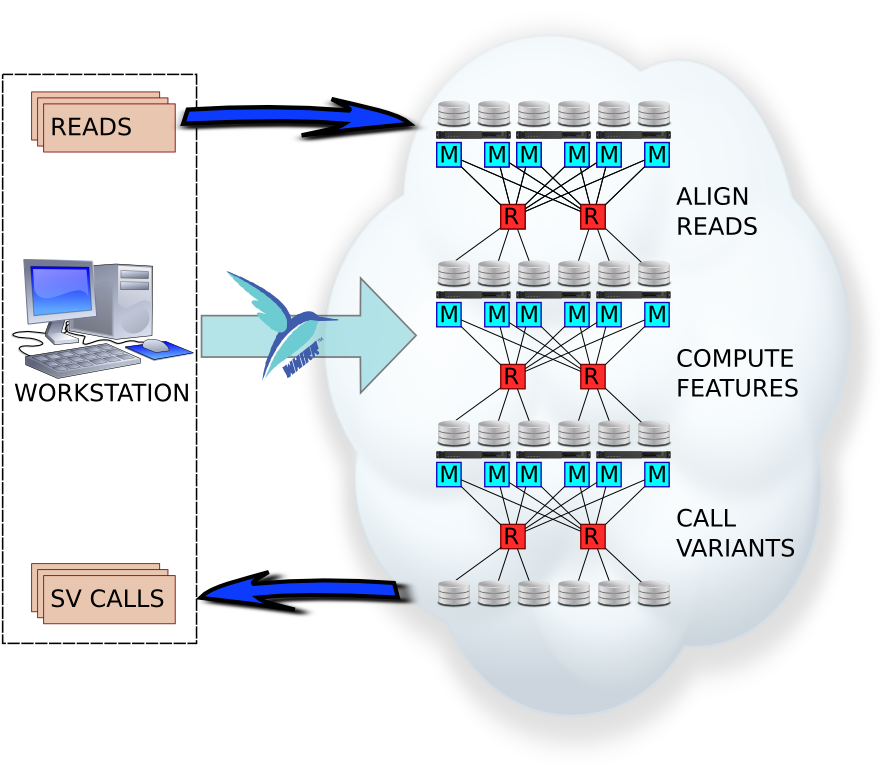
\includegraphics[width=.8\textwidth]{figures/workflow_with_whirr.png}
\caption{An overview of the Cloudbreak workflow. Reads are first uploaded to a Hadoop cluster from local storage. Cloudbreak then executes three MapReduce jobs to process the data: 1) Mapping with sensitive settings. 2) Computation of features across the genome. 3) Calling structural variations based on the features computed in the previous step. Finally, SV predictions can be downloaded from the Hadoop cluster and examined. Cloudbreak can also use the Apache Whirr library to automatically provision Hadoop clusters on and deploy data to cloud providers such as Amazon Elastic Compute Cloud.}
\label{cloudbreak_workflow}
\end{figure}


The \textsc{Align Reads} job uses existing alignment tools to discover mapping locations for each read pair. Aligners can be executed to report multiple possible mappings for each read, or only the best possible mapping. Given a set of read pairs, each of which consists of a read pair identifier $rpid$ and two sets of sequence and quality scores $<s,q>$, each mapper aligns each pair end set $<s,q>$ in either single- or paired end mode and emits possible mapping locations under the $rpid$ key. Reducers then collect the alignments for each paired end, making them available under one key for the next job. Our implementation of the framework contains wrappers to execute the aligners BWA \cite{Li:2009p836}, GEM \cite{MarcoSola:2012hm}, Novoalign \cite{novoalign}, RazerS 3 \cite{Weese:2012by}, mrFAST \cite{Alkan:2009cr}, and Bowtie 2 \cite{Langmead:2012jh}. This job can also be skipped in favor of importing a pre-aligned BAM file directly into HDFS.

In the \textsc{Compute Features} job, we compute a set of features for each location in the genome. To begin, we tile the genome with small fixed-width, non-overlapping intervals. For the experiments reported in this paper we use an interval size of 25bp. Let $L = \left\{l_1,l_2,\ldots,l_N\right\}$ be the set of intervals covering the entire genome. Let $R^1 = \left\{r^{1}_{1},r^{1}_{2},\ldots,r^{1}_{M}\right\}$ and $R^2 = \left\{r^{2}_{1},r^{2}_{2},\ldots,r^{2}_{M}\right\}$ be the input set of paired reads. Let $A^1 = \left\{a^{1}_{m,1},a^{1}_{m,2},\ldots,a^{1}_{m,K}\right\}$ and $A^2 = \left\{a^{2}_{m,1},a^{2}_{m,2},\ldots,a^{2}_{m,L}\right\}$ be the set of alignments for the left and right reads from read pair $m$. For any given pair of alignments of the two reads in a read pair, $a^{1}_{m,i}$ and $a^{2}_{m,j}$, let the $\textrm{ReadPairInfo } rpi_{m,i,j}$ be information about the pair relevant to detecting SVs, e.g. the fragment size implied by the alignments and the likelihood that the alignments are correct. We then leave two functions to be implemented depending on the application:
\begin{flalign*}
 \textsc{Loci } :& \langle a^{1}_{m,i},a^{2}_{m,j} \rangle \rightarrow L_m \subseteq L \\
 \Phi :& \left\{\textrm{ReadPairInfo }rpi_{m,i,j}\right\} \rightarrow \mathbb{R}^N \\
\end{flalign*}

The first function, \textsc{Loci}, maps an alignment pair to a set of genomic locations to which it is relevant for SV detection; for example, the set of locations overlapped by the internal insert implied by the read alignments.  We optimize this step by assuming that if there exist concordant mappings for a read pair, defined as those where the two alignments are in the proper orientation and with an insert size within three standard deviations of the expected library insert size, one of them is likely to be correct and therefore we do not consider any discordant alignments of the pair. The second function, $\Phi$, maps a set of ReadPairInfos relevant to a given location to a set of real-valued vectors of features useful for SV detection. 

Finally, the third MapReduce job, \textsc{Call Variants}, is responsible for making SV calls based on the features computed at each genomic location. It calls another application-specific function  $\textsc{PostProcess} : \left\{\phi_1,\phi_2,\ldots,\phi_N\right\} \rightarrow \left\{\langle  \textrm{SVType } s, l_{start}, l_{end} \rangle\right\}$  that maps the sets of features for related loci into a set of SV calls characterized by their type $s$ (i.e Deletion, Insertion, etc.) and their breakpoint locations $l_{start}$ and $l_{end}$. We parallelize this job in MapReduce by making calls for each chromosome in parallel, which we achieve by associating a location and its set of features to its chromosome in the map phase, and then making SV calls for one chromosome in each reduce task.

\begin{algorithm}[h]
\algrenewcommand\algorithmicprocedure{\textbf{job}}
 \begin{algorithmic}[1]
 \Procedure{Alignment}{}
 \Function{Map}{$\textrm{ReadPairId }rpid, \textrm{ReadId }r, \textrm{ReadSequence }s, \textrm{ReadQuality }q$}
 \ForAll{$ \textrm{Alignments }a \in \textsc{Align}(<s,q>)$}
 \State $\textsc{Emit}(\textrm{ReadPairId }rpid, \textrm{Alignment }a)$
 \EndFor
 \EndFunction
 \Function{Reduce}{$\textrm{ReadPairId }rpid, \textrm{Alignments }a_{1,2,\ldots}$}
 \State $\textrm{AlignmentPairList }ap \gets \textsc{ValidAlignmentPairs}(a_{1,2,\ldots})$
 \State $\textsc{Emit}(\textrm{ReadPairId }rp, \textrm{AlignmentPairList } ap)$
 \EndFunction
 \EndProcedure

 \Procedure{Compute SV Features}{}
 \Function{Map}{$\textrm{ReadPairId }rp, \textrm{AlignmentPairList }ap$}
 \ForAll{$ \textrm{AlignmentPairs }<a_1,a_2> \in ap$}
 \ForAll{$ \textrm{GenomicLocations }l \in \textsc{Loci }(a_1,a_2)$}
 \State $ \textrm{ReadPairInfo }rpi \gets <\textrm{InsertSize}(a_1,a_2), \textrm{AlignmentScore}(a_1,a_2)>$
 \State $\textsc{Emit}(\textrm{GenomicLocation }l, \textrm{ReadPairInfo }rpi)$
 \EndFor
 \EndFor
 \EndFunction
 \Function{Reduce}{$\textrm{GenomicLocation }l, \textrm{ReadPairInfos }rpi_{1,2,\ldots}$}
 \State $\textrm{SVFeatures } \phi_l \gets \Phi(\textrm{InsertSizes }i_{1,2,\ldots}, \textrm{AlignmentScores }q_{1,2,\ldots})$
 \State $\textsc{Emit}(\textrm{GenomicLocation }l, \textrm{SVFeatures } \phi_l)$
 \EndFunction
 \EndProcedure

 \Procedure{Call SVs}{}
 \Function{Map}{$\textrm{GenomicLocation }l, \textrm{SVFeatures } \phi_l$}
 \State $\textsc{Emit}(\textrm{Chromosome}(l), <l,\phi_l>)$
 \EndFunction
 \Function{Reduce}{$\textrm{Chromosome }c, \textrm{GenomicLocation } l_{1,2,\ldots},\phi_{1,2,\ldots}$}
 \State $\textrm{StructuralVariationCalls } svs_c \gets \textsc{PostProcess }(\phi_{1,2,\ldots})$
 \EndFunction
 \EndProcedure
 \end{algorithmic}
\caption{The algorithmic framework for SV calling in MapReduce.}
\label{cb_algo}
\end{algorithm}


% \chapter{Cloudbreak}\label{chap_cloudbreak_impl}

In the previous chapter, we described and formalized a general strategy for building SV detection algorithms in MapReduce and Hadoop. In this chapter, we describe an software package, Cloudbreak, that we have developed using this algorithmic framework. To build Cloudbreak, we implemented the infrastructure necessary to support the algorithmic framework we described in Section~\ref{section_general_algo}, and also provided implementations of the three application-specific functions we described there. Here we will describe this implementation, as well as our choices for the three user-defined functions we specified in the framework definition, and additional functionality we developed to genotype calls and to facilitate the deployment of Cloudbreak on public cloud platforms including Amazon's EC2. In Chapter~\ref{chap_cloudbreak_eval}, we will provide an evaluation of the algorithm's accuracy and performance characteristics.

\section{Variant types detected}

Cloudbreak is our implementation of a detection algorithm for genomic deletions (40bp-25,000bp) and small insertions based on examining the insert sizes of paired end mappings. We chose this application because small deletions in the range of 50bp to 150bp are particularly difficult to detect using many existing SV algorithms~\cite{Alkan:2011p547,Mills:2011fi}. This is because most read-pair based algorithms use a hard cutoff based on the variance of the fragment size distribution to select discordant read pairs, as described in Section~\ref{section_read_pair}. By taking advantage of many compute cores using MapReduce, we can design an algorithm that considers all of available data (both concordant and discordant read pairs) in a generative statistical framework, as we will describe in Section~\ref{section_user_defined_functions}.

\section{Framework infrastructure}

In addition to the specific algorithm for detecting deletions and insertions (which take the form of implementations of the user-defined functions we described in the previous chapter), the Cloudbreak package also contains the infrastructure necessary to implement the three MapReduce jobs defined in our MapReduce algorithmic framework. Providing a fully featured, multi-job Hadoop application requires several implementation decisions:

\begin{itemize}
\item \textbf{Programming language and method of interacting with Hadoop.} Hadoop applications can be developed in several ways. A native application is written in Java and directly uses the Hadoop application programming interface (API) to start jobs, implement Map and Reduce functions, and set advanced Hadoop configurations. Alternatively, applications can be developed in any language using the Hadoop \emph{streaming} interface, as long as the input to and output from all map and reduce tasks is textual and certain conventions are followed with respect to data format. Finally, for C/C++ applications, the Hadoop \emph{pipes} interface can be used to marshal input and output data from tasks. Each method has its own advantages and disadvantages. Native applications constrain the developer to Java but enjoy the best performance when the jobs are data intensive rather than CPU bound~\cite{Ding:2011:MCM:2103380.2103444}. Streaming applications allow greater programming language flexibility but make it somewhat more difficult to organize complex applications and take advantage of advanced Hadoop features. Pipes, meanwhile, allow for maximum performance for CPU intensive applications. We opted to develop Cloudbreak as a native application to take advantage of the tight integration with the Hadoop API improved I/O performance on data intensive portions of the workflow. For the \textsc{Align Reads} job, which executes existing short-read alignment tools, a mapper class written in Java invokes the external tools using the system runtime environment.

\item \textbf{File formats and compression.} Hadoop applications usually store their data in HDFS in text format or in sequence files, a binary format that allows numeric or complex data types to be stored in a key-value pair structure easily accessed by Hadoop. In addition, varying levels of compression can be used, although only certain compression types allow Hadoop to automatically split large files by HDFS blocks for processing by different map tasks, which is a key consideration for building fully parallelized applications. Cloudbreak uses sequence files for input and intermediate files, although for alignments the values are stored as text strings containing full records in the Sequence Alignment Map (SAM) format~\cite{Li:2009vz}, to allow for easy exports of data. For compression we use the Snappy~\cite{snappy} compressor/decompressor (codec), a compression scheme developed at Google which aims for reasonable file size reduction with very fast compression and decompression speeds. This makes it ideal for data-intensive Hadoop applications. Given that the output data from the \textsc{Align Reads} job is alignment records, a future implementation goal is to switch to using Hadoop-BAM~\cite{Niemenmaa:2012hu}, a library for storing SAM/BAM records efficiently in HDFS; Hadoop-BAM did not posses necessary functionality at the time of Cloudbreak's initial implementation and so we proceeded with a text-based representation of alignment records.

\item \textbf{Distribution of auxiliary files.} In some cases all tasks require access to large input files, such as genome reference indices for alignment, or genome annotation files. Hadoop offers a \emph{distributed cache} service, which places copies of the files on each node that will host tasks for the job so that they will not all need to copy the files over the network. Cloudbreak makes use of the distributed cache to distribute index and annotation files, as well as the alignment executables for the \textsc{Align Reads} job.
\end{itemize}

Our implementation of the \textsc{Align Reads} job contains wrappers to execute the aligners BWA \cite{Li:2009p836}, GEM \cite{MarcoSola:2012hm}, Novoalign \cite{novoalign}, RazerS 3 \cite{Weese:2012by}, mrFAST \cite{Alkan:2009cr}, and Bowtie 2 \cite{Langmead:2012jh}. This job can also be skipped in favor of importing a pre-aligned BAM file directly into HDFS. The code is structured in such a way that to add a new aligner, developers would simply create a class that finds the necessary index files in the distributed cache and determines the proper command line parameters for aligner execution, and parses the aligner output if it is in a non-standard format.

Cloudbreak can be executed on any Hadoop cluster; Hadoop abstracts away the details of cluster configuration, making distributed applications portable. We deployed Cloudbreak on an internal 56-node cluster running the Cloudera CDH3 Hadoop distribution, version 0.20.2-cdh3u4. In addition, Cloudbreak can create and operate on Hadoop clusters in the Amazon compute cloud (see Section~\ref{section_cloud_whirr}).

The source code and user manual for Cloudbreak are publicly available at \url{https://github.com/cwhelan/cloudbreak}. We hope that by publishing under an open-source license, we will facilitate the adoption of our Cloudbreak implementation, as well as provide a base from which other computational researchers can develop their own SV detection algorithms for Hadoop.

\section{Implementation of a MapReduce SV Algorithm}\label{section_user_defined_functions}

In Section~\ref{section_general_algo}, we described three user-defined functions that can be implemented to create an SV detection application in our MapReduce framework. These functions were named \textsc{Loci}, $\Phi$, and \textsc{PostProcess}. These functions map aligned read pairs to locations on the genome to which they are relevant, compute a set of local features for each genomic location based on the relevant read pairs, and call variants based on the features computed for neighboring genomic locations. Cloudbreak contains implementations of these functions that combine to allow it to detect deletions (of size 40bp-25,000bp) and insertions. A detailed description of each of these implementations appears below, and an illustration of each phase of the Cloudbreak algorithm working on a simple example in MapReduce is shown in Figure \ref{cloudbreak_example}.

\begin{figure}
\centering
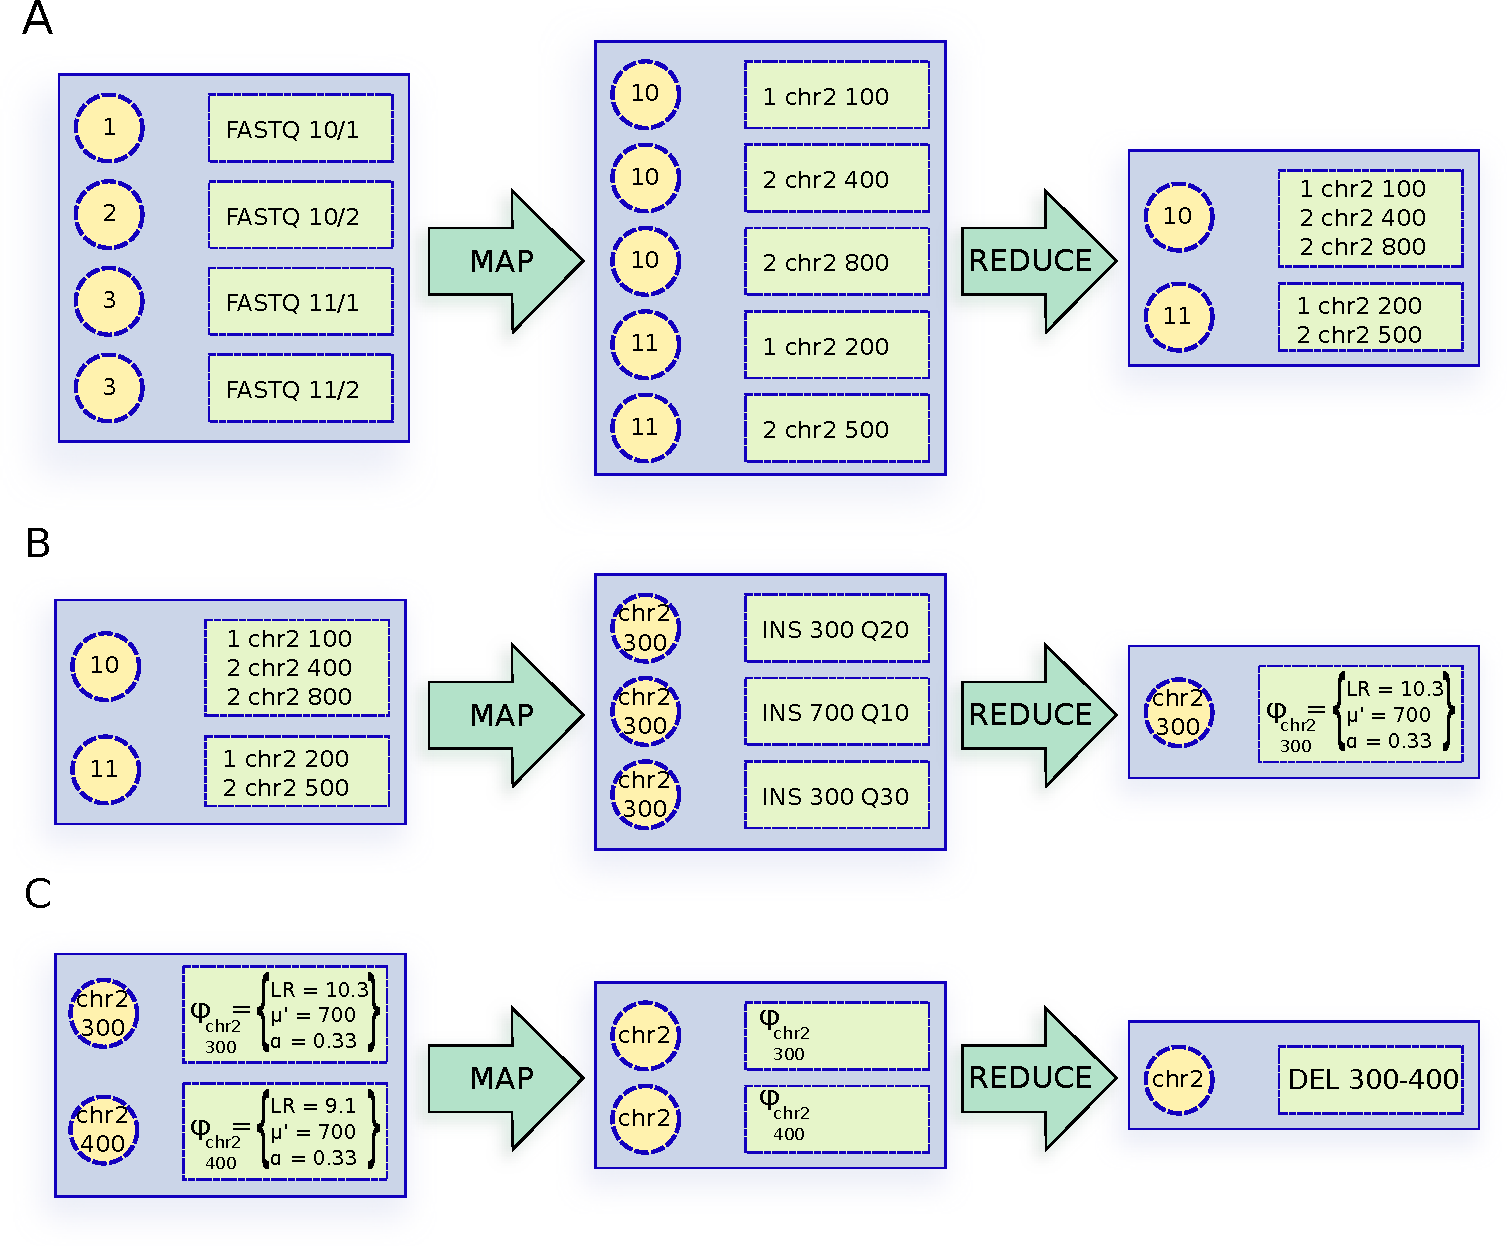
\includegraphics[width=.9\textwidth]{/users/cwhelan/Documents/svpipeline/figures/cloudbreak_mapred_diagram.pdf}
\caption{An Example of the Cloudbreak deletion and insertion detection algorithm running in MapReduce. A) In the first MapReduce job, mappers scan input reads in FASTQ format and execute an alignment program in either paired-end or single-ended mode to generate read mappings. Reducers gather all alignments for both reads in each pair. B) In the second MapReduce job, mappers first emit information about each read pair (in this case the insert size and quality) under keys indicating the genomic location spanned by that pair. Only one genomic location is diagrammed here for simplicity. Reducers then compute features for each location on the genome by fitting a GMM to the distribution of spanning insert sizes. C) Mappers group all emitted features by their chromosome, and reducers find contiguous blocks of features that indicate the presence of a variant.}
\label{cloudbreak_example}
\end{figure}

\begin{description}
\item[\sc{Loci}] Because we are detecting deletions and short insertions, we map ReadPairInfos from each possible alignment to the genomic locations overlapped by the implied internal insert between the reads. For efficiency, we define a maximum detectable deletion size of 25,000bp, and therefore alignment pairs in which the ends are more than 25kb apart, or in the incorrect orientation, map to no genomic locations. In addition, if there are multiple possible mappings for each read in the input set, we optimize this step by assuming that if there exists a concordant mapping for a read pair, defined as a mapping pair in which the two alignments are in the proper orientation and with an insert size within three standard deviations of the expected library insert size, it is likely to be correct and therefore we do not consider any discordant alignments of the pair.

\item[$\Phi$] To compute features for each genomic location, we follow the mixture of distributions approach (see Section~\ref{section_mixture_of_distributions}) first described by Lee et al.~\cite{Lee:2009da}, who observed that if all mappings are correct, the insert sizes implied by mappings which span a given genomic location should follow a Gaussian mixture model (GMM) whose parameters depend on whether a deletion or insertion is present at that locus. Figure~\ref{insert_size_mixes} shows several examples of the mixtures observed for various types of variants. If there is no indel, the insert sizes implied by spanning alignment pairs should follow the distribution of actual fragment sizes in the sample, which is typically modeled as normally distributed with mean $\mu$ and standard deviation $\sigma$. If there is a homozygous deletion or insertion of length $l$ at the location, $\mu$ should be shifted to $\mu + l$, while $\sigma$ will remain constant. Finally, in the case of a heterozygous event, the distribution of insert sizes will follow a mixture of two normal distributions, one with mean $\mu$, and the other with mean $\mu + l$, both with an unchanged standard deviation of $\sigma$, and mixing parameter $\alpha$ that describes the relative weights of the two components. The features generated for each location $l$ include the log-likelihood ratio of the filtered observed data points under the fit GMM to their likelihood under the distribution $N(\mu,\sigma)$, the final value of the mixing parameter $\alpha$, and $\mu'$, the estimated mean of the second GMM component. 

The choice of a mixture of distributions model has several benefits. Firstly, it is a generative model for the entire data set, including concordant and discordant read pairs. This removes the need to set hard thresholds that define discordant read pairs, and allows the detection of smaller variants given a tight enough insert size distribution. Second, the parameters that are estimated can be used to refine and classify predictions. For example, the mixing parameter $\alpha$ can be used to genotype variants, as we will describe in Section~\ref{section_genotyping}. In addition, the estimated $\mu'$ parameter gives a prediction for how many genomic locations the variant might cover, which we leverage in the \textsc{PostProcess} function described below to integrate local features into variant calls.

To implement our model, at each genomic location we fit the parameters of the GMM using the Expectation-Maximization algorithm. Let $Y = y_{1,2, \ldots m}$ be the observed insert sizes at each location after filtering, and say the library has mean fragment size $\mu$ with standard deviation $\sigma$. Because the mean and standard deviation of the fragment sizes are selected by the experimenter and therefore known \emph{a priori} (or at least easily estimated based on a sample of alignments), we only need to estimate the mean of the second component at each locus, and the mixing parameter $\alpha$. Therefore, we initialize the two components to have means $\mu$ and $\bar{Y}$, set the standard deviation of both components to $\sigma$, and set $\alpha = .5$. In the E step, we compute for each $y_i$ and GMM component $j$ the value $\gamma_{i,j}$, which is the normalized likelihood that $y_i$ was drawn from component $j$. We also compute $n_j = \sum_i{\gamma_{i,j}}$, the relative contributions of the data points to each of the two distributions. In the M step, we update $\alpha$ to be $n_2 - \left|Y\right|$, and set the mean of the second component to be $\frac{\sum_m{\gamma_{m,2}y_m}}{n_2}$. We treat the variance as fixed and do not update it, since under our assumptions the standard deviation of each component should always be $\sigma$. We repeat the E and M steps until convergence, or until a maximum number of steps has been taken. Prior to fitting the GMM at each location, we attempt to filter out incorrect mappings for that location using an outlier-detection based clustering scheme and an adaptive mapping quality cutoff; see Section~\ref{section_incorrect_and_ambiguous_mappings} for details.

\item[\sc{PostProcess}] The third MapReduce job is responsible for making SV calls based on the features defined above. We convert our features along each chromosome to insertion and deletion calls by first extracting contiguous genomic loci where the log-likelihood ratio of the two models is greater than a given threshold. To eliminate noise we apply a median filter with window size 5. We end regions when $\mu'$ changes by more than 60bp ($2\sigma$), and discard regions where the average value of $\mu'$ is less than $\mu$ or where the length of the region differs from $\mu'$ by more than $\mu$.
\end{description}

\begin{figure}
\centering
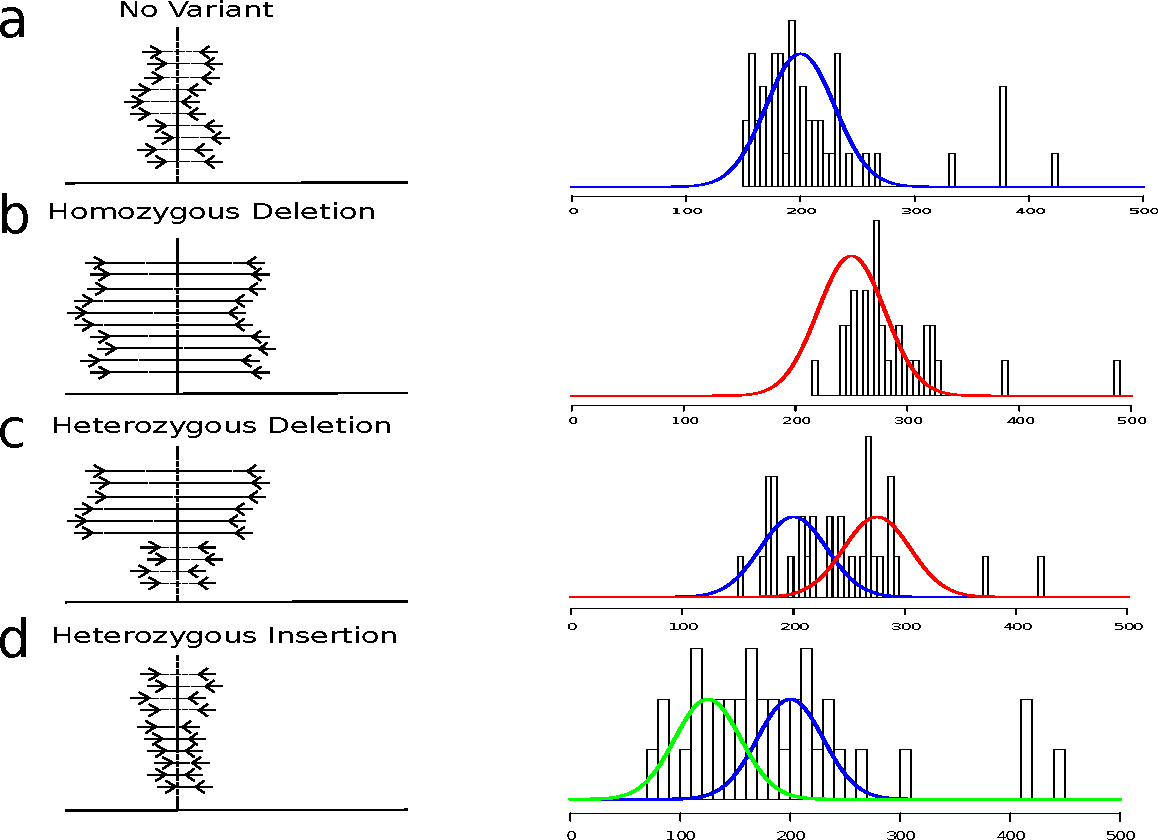
\includegraphics[width=.9\textwidth]{figures/insert_size_mixtures.pdf}
\caption{Illustration of insert size mixtures at individual genomic locations. A) there is no variant present at the location indicated by the vertical line (left), so the mix of insert sizes (right) follows the expected distribution of the library centered at 200bp, with a small amount of noise coming from low-quality mappings. B) a homozygous deletion of 50bp at the location has shifted the distribution of observed insert sizes. C) A heterozygous deletion at the location causes a mixture of normal and long insert sizes to be detected. D) A heterozygous small insertion shifts a portion of the mixture to have lower insert sizes.}
\label{insert_size_mixes}
\end{figure}

\section{Filtering Incorrect and Ambiguous Mappings}\label{section_incorrect_and_ambiguous_mappings}

One of our goals in developing Cloudbreak was to see if the use of distributed computing in the MapReduce framework would allow us to develop an algorithm that could process multiple mappings for ambiguously mapped reads in a reasonable amount of time, especially because the size of the dataset can grow very large if many possible mappings are kept for all ambiguous reads. Most SV detection tools that use multiple mappings attempt to identify the correct mapping for each ambiguously mapped pair; for example, GASVPro~\cite{Sindi:2012kk} uses an MCMC approach to sample from the distribution of possible mapping locations for each read, and VariationHunter~\cite{Hormozdiari:2009p284} attempts to assign mappings to reads through a combinatorial optimization approach. Cloudbreak, in contrast, attempts to solve this problem at the genomic location level by filtering mappings during the feature computation step.

To handle incorrect and ambiguous mappings, we assume that in general they will not form normally distributed clusters in the same way that correct mappings will, and therefore use an outlier detection technique to filter the observed insert sizes for each location. We sort the observed insert sizes and define as an outlier an observation whose $k$th nearest neighbor is more than $n\sigma$ distant, where $k = 3$ and $n = 5$. In addition, we rank all observations by the estimated probability that the mapping is correct and use an \emph{adaptive quality cutoff} to filter observations: we discard all observations where the estimated probability the mapping is correct is less than the score of the maximum quality observation minus a constant $c$. This allows the use of more uncertain mappings in repetitive regions of the genome while restricting the use of low-quality mappings in unique regions. Defining $\textsc{Mismatches}(a)$ to be the number of mismatches between a read and the reference genome in the alignment $a$, we approximate the probability $p^{k}_c$ of each end alignment being correct by:

\[ p^{k}_c(a^{k}_{m,i}) = \frac{\exp({-\textsc{Mismatches}(a^{k}_{m,i})/2)}}{\sum_j{\exp(-\textsc{Mismatches}(a^{k}_{m,j})/2)}} \]

And then multiply $p_c(a^{1}_{m,i})$ and $p_c(a^{2}_{m,i})$ to approximate the likelihood that the pair is mapped correctly.

\section{Genotyping}\label{section_genotyping}

In theory, it should be possible to use the parameters of the fit GMM to infer the genotype of each predicted variant. Assuming that our pipeline is capturing all relevant read mappings near the locus of the variant, the genotype should be indicated by the estimated parameter $\alpha$, the mixing parameter that controls the weight of the two components in the GMM.  We set a simple cutoff on the average value of $\alpha$ for each prediction to call the predicted variant homozygous or heterozygous, and use the same cutoff for deletion and insertion predictions. Somewhat surprisingly, we observed on the cutoff point that distinguishes homozygous from heterozygous variants is significantly less than the expected .5; based on empirical observations on a simulated data set, we set the threshold to .35 (see Section~\ref{section_genotyping_eval} for more details).

\section{Running in the Cloud}\label{section_cloud_whirr}

In Section~\ref{section_seq_big_data}, we discussed the increasing recognition of the genomics community of the need for tools that ease the use of cloud computing resources~\cite{Schatz:2010js,Stein:2010gp}. This has spurred the development of a variety of applications and toolkits that use the APIs of Infrastructure as a Service (IaaS) providers, such as Amazon EC2, to allocate compute resources on public compute clouds. In this section, we will briefly review some of the existing cloud-enabled tools, including those that are based on traditional grid scheduling engines and those that enable Hadoop and MapReduce pipelines. Many of the latter take advantage of Amazon's Elastic MapReduce (EMR) service, an offering from Amazon specifically for creating and running Hadoop jobs that simplifies the creation and monitoring of clusters on EC2. We will then discuss how Cloudbreak enables the use of cloud computing in a provider-neutral way using the Apache Whirr library.

\subsection{Cloud-Enabled Genomics Tools}

Severak groups have created general-purpose toolkits for creating, allocating, and managing cloud resources for biological data processing. For example, the CloudBioLinux project~\cite{Krampis:2012wo} provides virtual machine images for use in Amazon EC2 that are pre-configured with a wide range of open-source bioinformatics applications. Galaxy CloudMan~\cite{Afgan:2010fa} allows for the automatic creation of clusters in the Amazon cloud configured to run workflows in the popular Galaxy environment~\cite{Giardine:2005ig}, backed by the SGE grid scheduling engine and with interfaces to Amazon's S3 storage service. CloVR~\cite{Angiuoli:2011wl} is a newer cloud cluster manager that includes several pipelines for metagenomics managed by SGE. Finally, Elastream~\cite{Issa:2013jp} is a newer offering that can provision and manage cloud clusters using either grid schedulers or EMR. 

Several commercial providers are also offering services that allow elastic cloud computing for sequencing pipelines, including DNAnexus (Mountain View, CA), Illumina's (San Diego, CA) BaseSpace cloud, Seven Bridges Genomics' (Cambridge, MA) IGOR platform, and an offering from Biodatomics (Bethesda, MD). These commercial cloud services are in many cases backed by Amazon's EC2, but are wrapped in additional sequencing-specific APIs and user interfaces by the vendor. To our knowledge Biodatomics is the only commercial bioinformatics vendor that offers automatic Hadoop cluster provisioning, however. 

There are also a number of bioinformatics suites designed for specific applications that are able to allocate resources on EC2 automatically. Apart from those that use Hadoop, which we will discuss in the next paragraph, these include: Atlas2 Cloud~\cite{Evani:2012eq}, which allows users to run the Genboree Workbench workflow for variant calling and annotation in personal genomics DNA resequencing projects; SIMPLEX~\cite{Fischer:2012bt}, which enables cloud processing for an exome alignment and variant calling pipeline based on BWA and the GATK; a set of ChIP-seq tools of the modENCODE and ENCODE projects~\cite{Trinh:2013ii} that can create clusters to run analysis pipelines on EC2 or the Bionumbus private cloud~\cite{bionimbus}.

Finally, several of the Hadoop applications we discussed in Section~\ref{section_mapred_related_work} come with command-line or graphical interfaces that automate their deployment on commercial cloud services. Most of these leverage EMR. The most widely used EMR-enabled tool is Crossbow~\cite{Langmead:2009p1225}, which has a UI that will create Hadoop workflows using EMR. Crossbow's ability to use EMR was recently made more robust by Rainbow~\cite{Zhao:2013hj}, which wraps Crossbow with additional facilities for transferring large files in parallel, monitoring clusters for failing nodes, and aggregating results from multiple samples run simultaneously. As mentioned in Section~\ref{section_mapred_related_work}, FX~\cite{Hong:2012du} and Euolsan~\cite{Jourdren:2012dc} are both Hadoop workflows for RNA-seq processing; both have the ability to automatically create EMR jobs on Amazon EC2.

\subsection{Enabling Cloud Computing with Whirr}

In contrast to the tools mentioned above, Cloudbreak leverages the Apache Whirr~\cite{whirr} library to automatically create Hadoop clusters in the cloud. Whirr differs from the strategies referred to in the last section in that it provides a unified application programming interface (API) for provisioning and running cloud services that is agnostic to the cloud IaaS provider. Although the largest and most popular cloud IaaS is provided by Amazon Web Services though their Elastic Compute Cloud (EC2), Whirr is a facade API that allows the transparent substitution of other cloud services such as Rackspace, Microsoft Azure, or private clouds such as those built with Eucalyptus. Most of the Hadoop-enabled applications and toolkits mentioned in the previous section depend on Amazon Elastic MapReduce to provision Hadoop clusters. Cloudbreak's use of Whirr breaks this dependency on a single vendor.

Using Whirr's API, Cloudbreak can provision of Hadoop clusters which can then be terminated when processing is complete. This eliminates the need to invest in a standing cluster and allows a model in which users can scale their computational infrastructure as their need for it varies over time. Through a command line interface, Cloudbreak uses Whirr functionality to offer commands that:

\begin{itemize}
\item \textbf{Automatically provision Hadoop clusters in the cloud.} After specifying the parameters of the Hadoop cluster desired in a property file, a single Cloudbreak command will request the creation of the necessary compute instances in the cloud, will configure them with the proper Hadoop services to provide a fully functioning cluster, and will start proxies that make the Hadoop cluster's management and reporting UIs available to the user. Cloudbreak users can configure clusters with their credentials for the cloud service provider, the number of worker nodes to include in the cluster as well the hardware requirements for each node, and, if desired, the pricing model. This last point is particularly useful on EC2, where spot pricing allows users to bid for unclaimed compute capacity on Amazon's cloud. Spot pricing can dramatically reduce costs compared to full price on-demand instances. The disadvantage is that instances can be reallocated if a higher bid comes in, resulting in termination of the processes they are running. Hadoop's facility for automatic redundancy of data and tasks can mitigate this risk.

\item \textbf{Transfer data into cloud compute clusters.} Typically when using cloud compute services it is fastest to store large data sets in a cloud storage service such as Amazon's Simple Storage Service (S3). From there it is fast to transfer them into and out of cloud compute services like EC2. However, moving data into S3 can be time-consuming depending on the network connections and number and size of the files in the data set. Cloudbreak includes code which communicates with S3 to do a multi-threaded upload of large data files, enabling much faster transfer times.

\item \textbf{Destroy clusters when processing is complete.} Cloudbreak, by using the Whirr API, can destroy allocated cloud clusters when processing is complete, ensuring that compute costs can be managed efficiently.
\end{itemize}

Cloudbreak's user manual contains detailed instructions and examples describing how to leverage cloud computing. We hope that by making cloud computing readily accessible through Cloudbreak's command line interface, more researchers will have the opportunity to leverage Hadoop's distributed computing model, even if they do not have local Hadoop clusters available at their institutions.

\section{Discussion}

The strategy of fitting a GMM to the distribution of insert sizes at a given genomic location has been used by the SV detection tools MoDIL~\cite{Lee:2009da} and SVM$^2$~\cite{Chiara:2012ey}. SVM$^2$ fits a mixture of distributions only to candidate regions of the genome identified through a preliminary analysis for the purpose of genotyping variants as homozygous or heterozygous. This leaves MoDIL as the only tool that attempts to model the distribution of insert sizes across the entire genome. As we will see in the next chapter, MoDIL is prone to excessively long run times that make it impractical to run for large-scale genomics data sets. Cloudbreak, on the other hand, through its use of MapReduce and Hadoop, is able to efficiently distribute computation so that given a sufficiently large cluster it can deliver the benefits of this strategy with very fast runtimes.

For those researchers that wish to take advantage of cloud computing in order to avoid the expense and maintenance costs of running their own large Hadoop clusters, Cloudbreak is able to automatically provision, transfer data to, and destroy Hadoop clusters using IaaS providers. Although there are other cloud-enabled sequencing analysis tools, Cloudbreak is unique in using the Apache Whirr library to provide an IaaS provider-agnostic solution. In addition to the obvious benefit of avoiding vendor lock-in, we believe that this will become increasingly important in the future as research agencies and clinical providers increasingly set up private or semi-private clouds to manage the analysis of sensitive personal genomic data in a controlled setting.
\chapter{Cloudbreak}

Cloudbreak is our implementation, in the framework described above, of a detection algorithm for genomic deletions (40bp-25,000bp) and small insertions based on examining the insert sizes of paired end mappings. An illustration of the Cloudbreak algorithm working on a simple example is shown in Figure 2.

\section{Implementation of the MapReduce SV Framework}

In particular, we implement the three user-defined functions specified above as follows:

\begin{description}
\item[\sc{Loci}] Because we are detecting deletions and short insertions, we map ReadPairInfos from each possible alignment to the genomic locations overlapped by the implied internal insert between the reads. For efficiency, we define a maximum detectable deletion size of 25,000bp, and therefore alignment pairs in which the ends are more than 25kb apart, or in the incorrect orientation, map to no genomic locations. In addition, if there are multiple possible mappings for each read in the input set, we optimize this step by assuming that if there exists a concordant mapping for a read pair, defined as a mapping pair in which the two alignments are in the proper orientation and with an insert size within three standard deviations of the expected library insert size, it is likely to be correct and therefore we do not consider any discordant alignments of the pair.
\item[$\Phi$] To compute features for each genomic location, we follow Lee et al. \cite{Lee:2009da}, who observed that if all mappings are correct, the insert sizes implied by mappings which span a given genomic location should follow a Gaussian mixture model (GMM) whose parameters depend on whether a deletion or insertion is present at that locus (Figure A1). Briefly: if there is no indel, the insert sizes implied by spanning alignment pairs should follow the distribution of actual fragment sizes in the sample, which is typically modeled as normally distributed with mean $\mu$ and standard deviation $\sigma$. If there is a homozygous deletion or insertion of length $l$ at the location, $\mu$ should be shifted to $\mu + l$, while $\sigma$ will remain constant. Finally, in the case of a heterozygous event, the distribution of insert sizes will follow a mixture of two normal distributions, one with mean $\mu$, and the other with mean $\mu + l$, both with an unchanged standard deviation of $\sigma$, and mixing parameter $\alpha$ that describes the relative weights of the two components. The features generated for each location $l$ include the log-likelihood ratio of the filtered observed data points under the fit GMM to their likelihood under the distribution $N(\mu,\sigma)$, the final value of the mixing parameter $\alpha$, and $\mu'$, the estimated mean of the second GMM component. See Methods for more details on the GMM fitting procedure. Prior to fitting the GMM at each location, we attempt to filter our incorrect mappings for that location using an outlier-detection based clustering scheme and an adaptive mapping quality cutoff (see Methods for details).

\item[\sc{PostProcess}] The third MapReduce job is responsible for making SV calls based on the feature defined above. We convert our features along each chromosome to insertion and deletion calls by first extracting contiguous genomic loci where the log-likelihood ratio of the two models is greater than a given threshold. To eliminate noise we apply a median filter with window size 5. We end regions when $\mu'$ changes by more than 60bp ($2\sigma$), and discard regions where the average value of $\mu'$ is less than $\mu$ or where the length of the region differs from $\mu'$ by more than $\mu$.
\end{description}



\begin{figure}
\centering
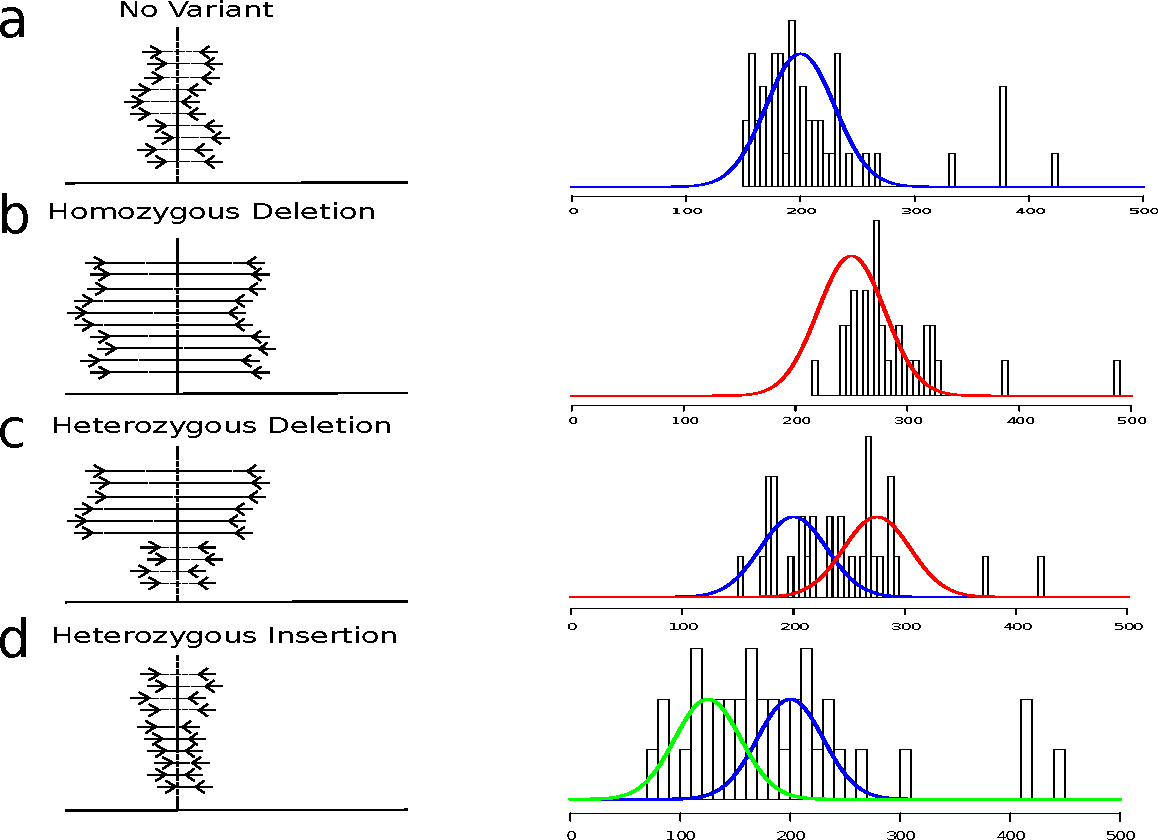
\includegraphics[width=.9\textwidth]{figures/insert_size_mixtures.pdf}
\caption{Illustration of insert size mixtures at individual genomic locations. A) there is no variant present at the location indicated by the vertical line (left), so the mix of insert sizes (right) follows the expected distribution of the library centered at 200bp, with a small amount of noise coming from low-quality mappings. B) a homozygous deletion of 50bp at the location has shifted the distribution of observed insert sizes. C) A heterozygous deletion at the location causes a mixture of normal and long insert sizes to be detected. D) A heterozygous small insertion shifts a portion of the mixture to have lower insert sizes.}
\label{insert_size_mixes}
\end{figure}


\section{Incorrect and ambiguous mappings}

To handle incorrect and ambiguous mappings, we assume that in general they will not form normally distributed clusters in the same way that correct mappings will, and therefore use an outlier detection technique to filter the observed insert sizes for each location. We sort the observed insert sizes and define as an outlier an observation whose $k$th nearest neighbor is more than $n\sigma$ distant, where $k = 3$ and $n = 5$. In addition, we rank all observations by the estimated probability that the mapping is correct and use an \emph{adaptive quality cutoff} to filter observations: we discard all observations where the estimated probability the mapping is correct is less than the score of the maximum quality observation minus a constant $c$. This allows the use of more uncertain mappings in repetitive regions of the genome while restricting the use of low-quality mappings in unique regions. Defining $\textsc{Mismatches}(a)$ to be the number of mismatches between a read and the reference genome in the alignment $a$, we approximate the probability $p^{k}_c$ of each end alignment being correct by:

\[ p^{k}_c(a^{k}_{m,i}) = \frac{\exp({-\textsc{Mismatches}(a^{k}_{m,i})/2)}}{\sum_j{\exp(-\textsc{Mismatches}(a^{k}_{m,j})/2)}} \]

And then multiply $p_c(a^{1}_{m,i})$ and $p_c(a^{2}_{m,i})$ to approximate the likelihood that the pair is mapped correctly.

% \input{evaluation}
\section{Evaluation}


\subsection{Choice of Methods to Compare To}

We compared the performance of Cloudbreak for detecting deletions and insertions to a selection of popular tools: the RP method BreakDancer \cite{Chen:2009p3}, GASVPro, an RP method that integrates RD signals and ambiguous mappings \cite{Sindi:2012kk}, the SR method Pindel \cite{Ye:2009p2}, and the hybrid RP-SR method DELLY \cite{Rausch:2012he}. DELLY produces two sets of calls, one based solely on RP signals, and the other based on RP calls that could be supported by SR evidence; we refer to these sets of calls as DELLY-RP and DELLY-SR. We also attempted to evaluate MoDIL on the same data. All of these methods detect deletions. Insertions can be detected by BreakDancer, Pindel, and MoDIL. See Methods for details on how reads were aligned and each program was invoked. For all alignments we used BWA, although in testing Cloudbreak we have found that the choice of aligner, number of possible mapping locations reported, and whether the reads were aligned in paired-end or single-ended mode can have a variety of effects on the output of the algorithm \ref{alignment_comparison}.

\subsection{A Note on Comparing and Evaluating Performance and Runtime}

We implemented and executed Cloudbreak on a 56-node Hadoop cluster, with 636 map slots and 477 reduce slots. Not including alignment time, we were able to process the Chromosome 2 simulated data in under five minutes, and the the NA18507 data set in under 15 minutes. For the simulated data set we used 100 reducers for the compute SV features job; for the real data set we used 300. The bulk of Cloudbreak's execution is spent in the feature generation step. Extracting deletion and insertion calls take under two minutes each for both the real and simulated data sets; the times are equal because each reducer is responsible for processing a single chromosome, and so the runtime is bounded by the length of time it takes to process the largest chromosome. 

In Table \ref{runtimes} we display a comparison of runtimes on the real and simulated data sets for all of the tools evaluated in this work. Each tool varies in the amount of parallelization supported. We report runtimes for tools run in their default single-threaded mode, as well as for levels of parallelization achievable with basic scripting, noting that one of the key advantages of Hadoop/MapReduce is the ability to scale parallel execution to the size of the available compute cluster without any custom programming. Pindel allows multi-threaded operation on multicore servers. Pindel and Breakdancer allow processing of a single chromosome in one process, so it is possible to execute all chromosomes in parallel on a cluster that has a job scheduler and shared filesystem. Breakdancer has an additional preprocessing step (\texttt{bam2cfg.pl}) which runs in a single thread. DELLY suggests splitting the input BAM file by chromosome, after which a separate DELLY process can be executed on the data for each chromosome; splitting a large BAM file is a time consuming process and consumes most of the time in this parallel workflow, in fact making it faster to run in single-threaded mode. GASVPro allows parallelization of the MCMC component for resolving ambiguously mapped read pairs; however, this requires a significant amount of custom scripting, and we did not find that the MCMC module consumed most of the runtime in our experiments, so we do not attempt to parallelize this component. The MoDIL distribution contains a set of scripts that can be used to submit parallel jobs to the SGE scheduling engine or modified for other schedulers; we adapted these for use in our cluster.

\begin{table}
\begin{center}
\begin{tabular}{r|r|rrr|rrr}
\multicolumn{2}{c}{}  & \multicolumn{3}{c}{Simulated Data} & \multicolumn{3}{c}{NA18507} \\
\hline
 & SV Types &  Single CPU & Parallel & Proc. &  Single CPU & Parallel & Proc.  \\ 
  \hline
  Cloudbreak & D,I &   NA    & 290 & 312    & NA         & 824 & 636 \\ 
  Breakdancer & D,I,V,T &  653   & NA       & NA          & 134,170 &  5,586 & 84 \\
  GASVPro & D,V   &  3,339  & NA       & NA         & 52,385  & NA & NA \\
  DELLY & D         &  1,964 & NA          & NA      & 30,311  & 20,224 & 84 \\
  Pindel & D,I,V,P         & 37,006 &  4,885     & 8          &  284,932  & 28,587 & 84 \\ 
  MoDIL & D,I        &  NA      & 52,547 & 250 & NA         & NA  & NA\\ 
   \hline
\end{tabular}
\end{center}
\caption{Runtimes (elapsed) on both data sets of each tool tested, in single-processor and parallel mode. For parallel runs, Proc. is the maximum number of simultaneously running processes or threads. All times are in seconds. The types of variants detected by each program are listed with the abbreviations: D - deletion; I - insertion; V - Inversion; P - duplication; T - translocation. Interchromosomal translocations are only detected by Breakdancer in single CPU mode. }
\label{runtimes}
\end{table}

In parallel execution, the total time to execute is bounded by the runtime of the longest-running process. In the case of chromosome-parallelizable tools including Breakdancer, Pindel, and DELLY, this is typically the process working on the largest chromosome.\footnote{We note that one Breakdancer process, handling an unplaced contig in the hg19 reference genome, never completed in our runs and had to be killed manually; we exclude that process from our results.} In the case of MoDIL's run on the simulated data, we found that the different processes varied widely in their execution times, likely caused by regions of high coverage or with many ambiguously mapped reads. Cloudbreak mitigates this problem during the time-consuming feature generation process by using Hadoop partitioners to randomly assign each genomic location to one of the set of reducers, ensuring that the work is evenly distributed across all processes. This distribution of processing across the entire cluster also serves to protect against server slowdowns and hardware failures - for example, we were still able to complete processing of the NA18507 data set during a run where one of the compute nodes was rebooted midway through the feature generation job.


\subsection{Tests with Simulated Data}

\begin{figure}
\centering
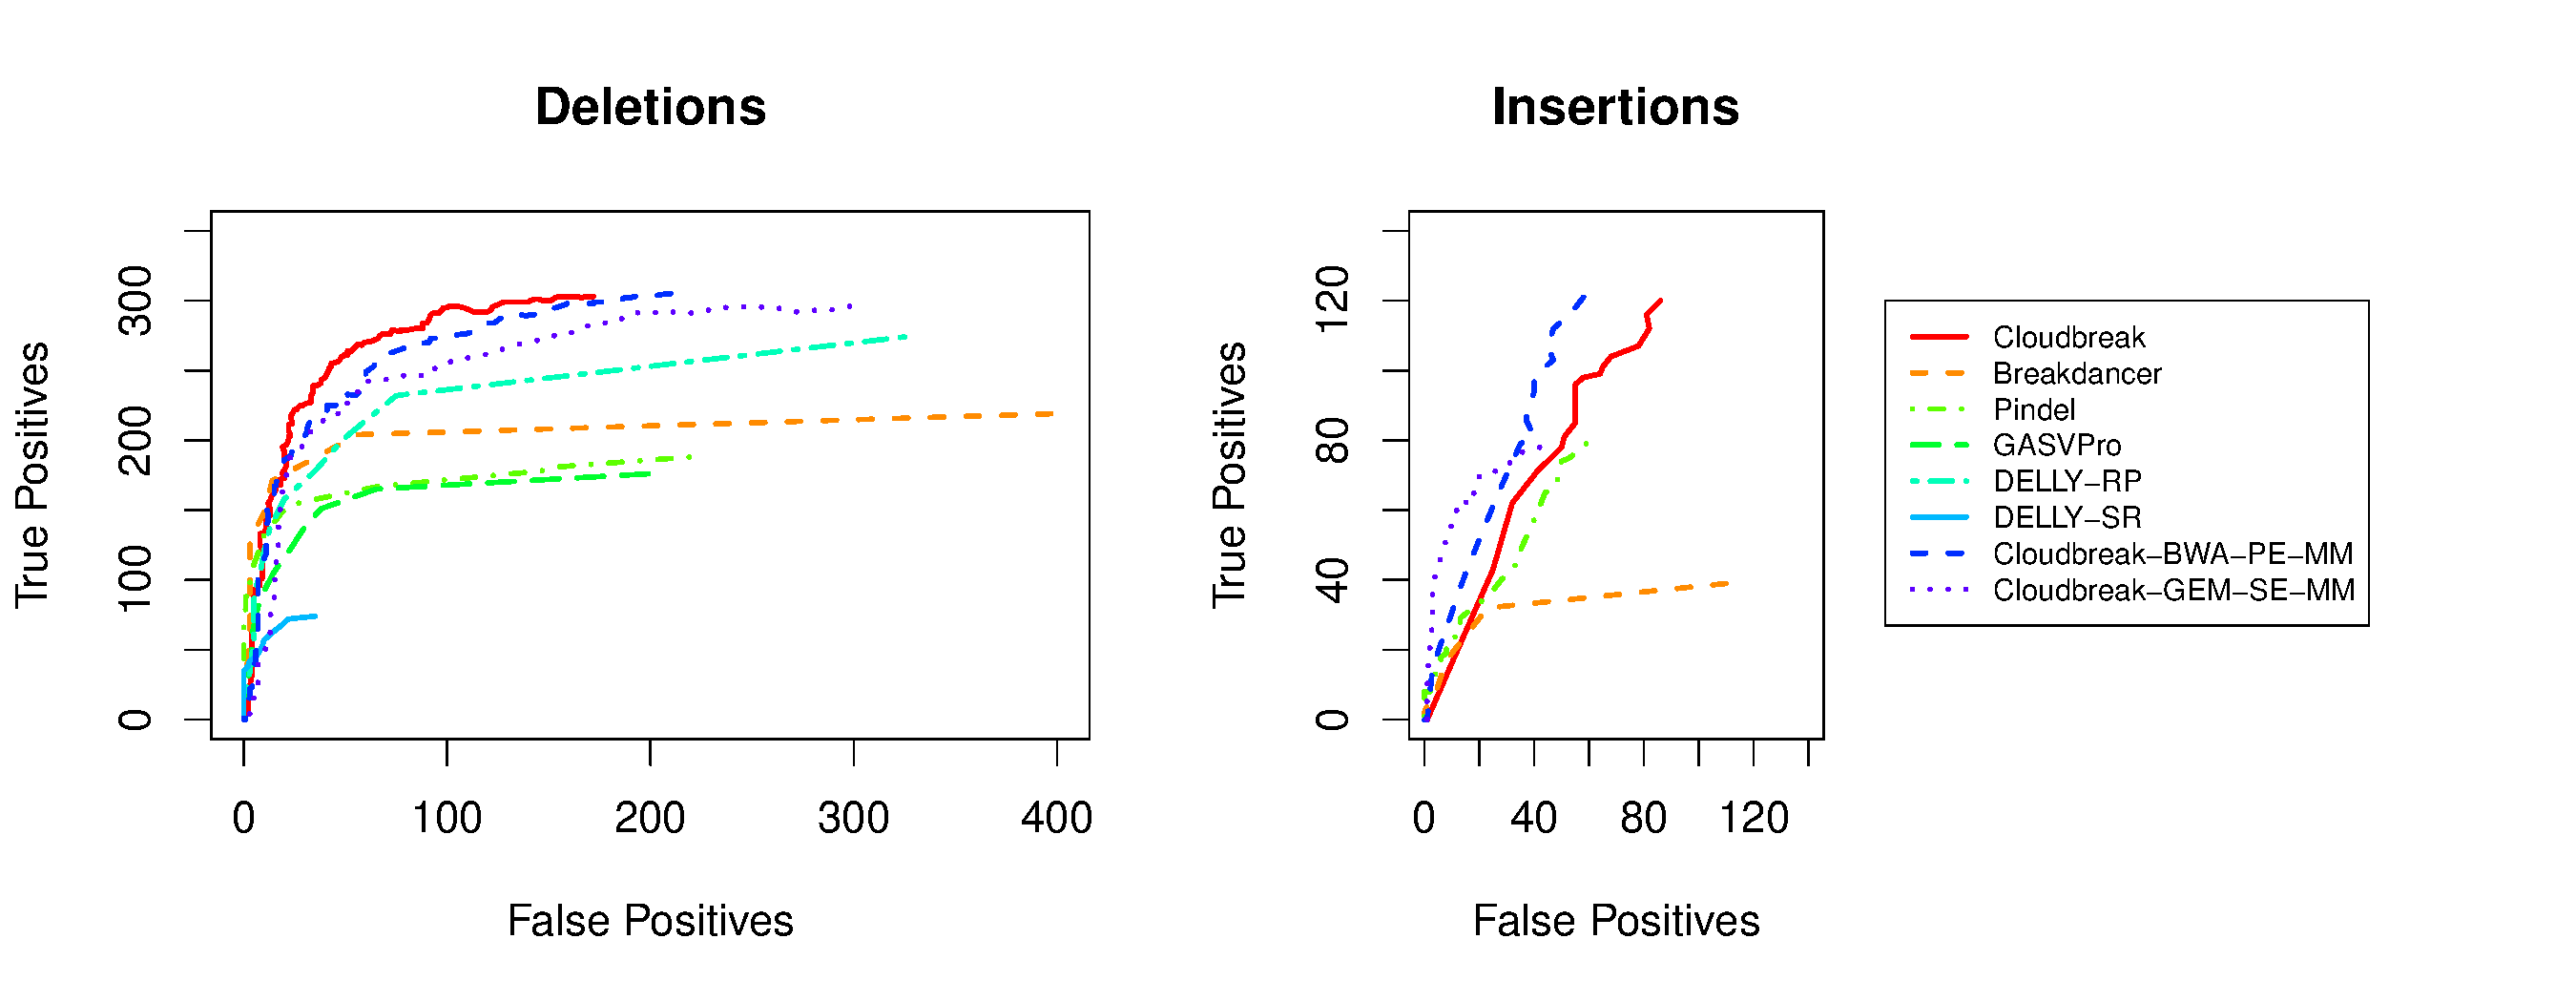
\includegraphics[width=1\textwidth]{/Users/cwhelan/Documents/svpipeline/figures/CHR2SIM_ROCS_MULTIPLE_MAPPINGS.pdf}
\caption{Cloudbreak performance on the chromosome 2 simulation using different alignment strategies. ROC curves show the number of true positives and false positives for each operating point for deletions and insertions. The Cloudbreak alignment strategies are: 1) ``Cloudbreak'': Alignments generated with BWA in paired-end mode, reporting the best hit for each pair. 2) ``Cloudbreak-BWA-PE-MM'': Alignments generated with BWA in paired-end mode, reporting up to 25 additional hits for each mapping in SAM format using the \texttt{-n} and \texttt{-N} parameters for \texttt{bwa sampe} and the script \texttt{xa2multi.pl}. 3) ``Cloudbreak-GEM-SE-MM'': Alignments generated by running the GEM aligner in single-ended mode, reporting up to 1000 additional hits per alignment. GEM was executed in parallel using Hadoop tasks which wrap GEM version 1.362 (beta), with parameters \texttt{-e 6 -m 6 -s 2 -q ignore -d 1000 --max-big-indel-length 0},  requesting all hits for a read that are within an edit distance of 6 of the reference, within 2 strata of the best hit, with a maximum of 1000 possible alignments reported for each read. Considering multiple mappings improves Cloudbreak's specificity for insertions but decreases sensitivity to deletions.}
\label{alignment_comparison}
\end{figure}

%, although in testing Cloudbreak we have found that the choice of aligner, number of possible mapping locations reported, and whether the reads were aligned in paired-end or single-ended mode can have a variety of effects on the output of the algorithm (Supplementary Figure~\ref{Salignment_comparison}).

As has been observed elsewhere, there is no available test set of real Illumina sequencing data from a sample that has a complete annotation of structural variations from the reference. Therefore, testing with simulated data is important to fully characterize an algorithm's performance characteristics. On the other hand, it is important that the simulated data contain realistic SVs that follow patterns of SVs observed in real data. To address this, we took one of the most complete lists of SVs from a single sample available, the list of homozygous insertions and deletions from the genome of J. Craig Venter~\cite{Levy:2007fb}. Using these variants, we simulated a 30X read coverage data set for a diploid human Chromosome 2 with a mix of homozygous and heterozygous variants, with 100bp reads and a mean fragment size of 300bp.

\begin{figure}
\centering
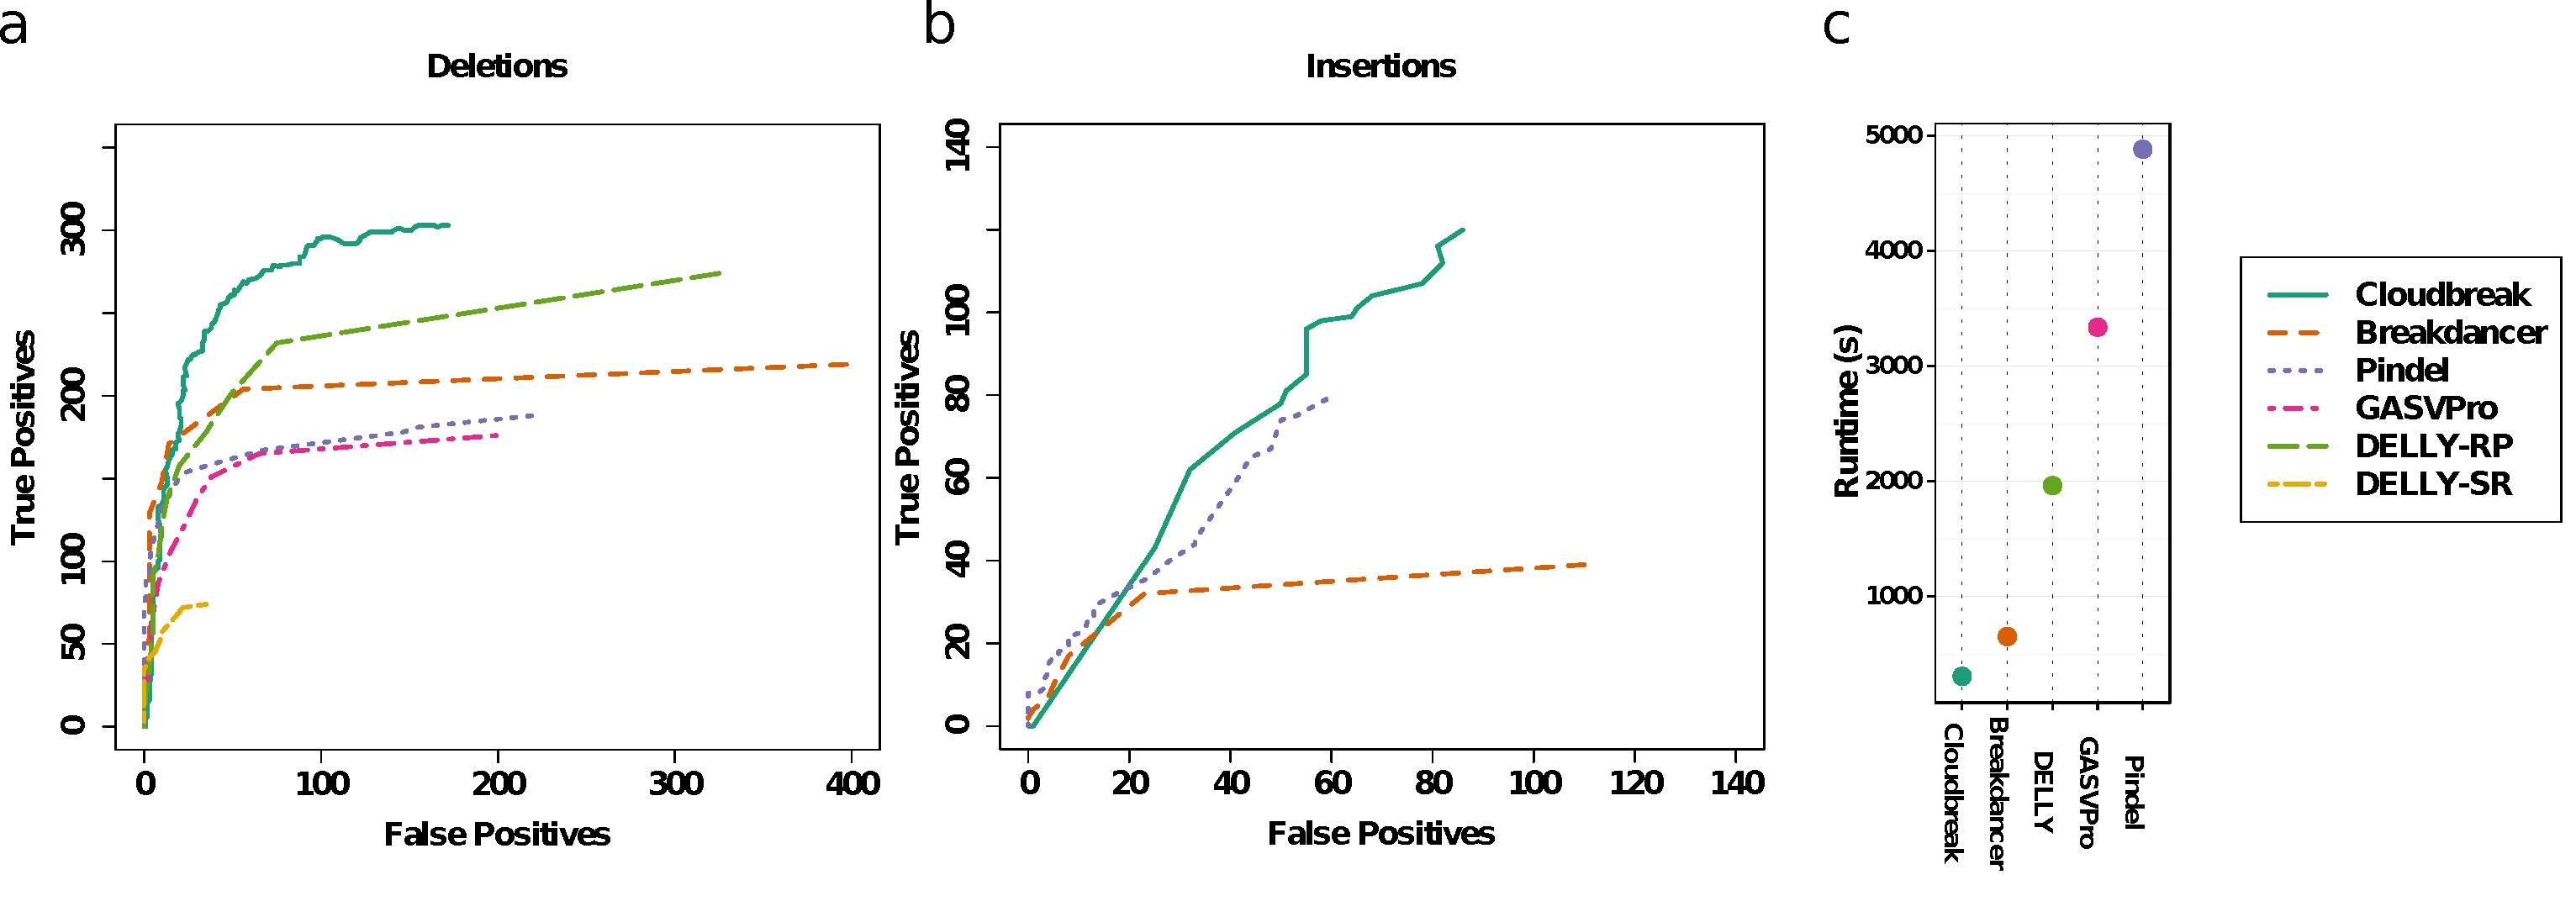
\includegraphics[width=1\textwidth]{figures/chr2_sim_rocs_runtime.pdf}
\caption{Accuracy and runtime performance on a simulated data set. (a) Receiver Operating Characteristic (ROC) curves showing the specificity and sensitivity of each tool to deletions larger than 40bp on a simulated set of reads giving diploid coverage of 30X on human chromosome 2. Deletions from the Venter genome were randomly added to one or both haplotypes. Each point on a curve represents a different threshold on the confidence of predictions made by that tool. Thresholds vary by: Cloudbreak - likelihood ratio; BreakDancer, DELLY, GASVPro - number of supporting read pairs; Pindel - simple score. (b) ROC curves for insertion predictions. (c) Runtimes for each tool, not including alignment time, parallelized when possible.}
\label{chr2CombinedRoc}
\end{figure}

Figure~\ref{chr2CombinedRoc} shows Receiver Operating Characteristics (ROC) curves of the performance of each algorithm for detecting deletions and insertions on the simulated data set, as well as the runtimes of the approaches tested, excluding alignment. See Methods for a description of how we identified correct predictions. All approaches show excellent specificity at high thresholds in this simulation. Cloudbreak provides the greatest specificity for deletions at higher levels of sensitivity, followed by DELLY. For insertions, Cloudbreak clearly provides the best combinations of sensitivity and specificity. Cloudbreak's runtime is half that of BreakDancer, the next fastest tool, processing the simulated data in under six minutes. (Of course, Cloudbreak uses many more CPUs as a distributed algorithm). \todo{See Supplementary Material and Supplementary Table~\ref{Sruntimes} for a discussion of runtimes and parallelization.} The output which we obtained from MoDIL did not have a threshold that could be varied to correlate with the trade-off between precision and recall and therefore it is not included in ROC curves; in addition, MoDIL ran for 52,547 seconds using 250 CPUs in our cluster, so results are not included in the runtime figure. Apart from the alignment phase, which is embarrassingly parallel, the feature generation job is the most computationally intensive part of the Cloudbreak workflow. \todo{Therefore, to test scalability we measured the runtime of that job on Hadoop clusters made up of varying numbers of nodes and observed that linear speedups can be achieved in this portion of the algorithm by adding additional nodes to the cluster until a point of diminishing returns is reached (Figure~\ref{scalability}).}

\begin{figure}
\centering
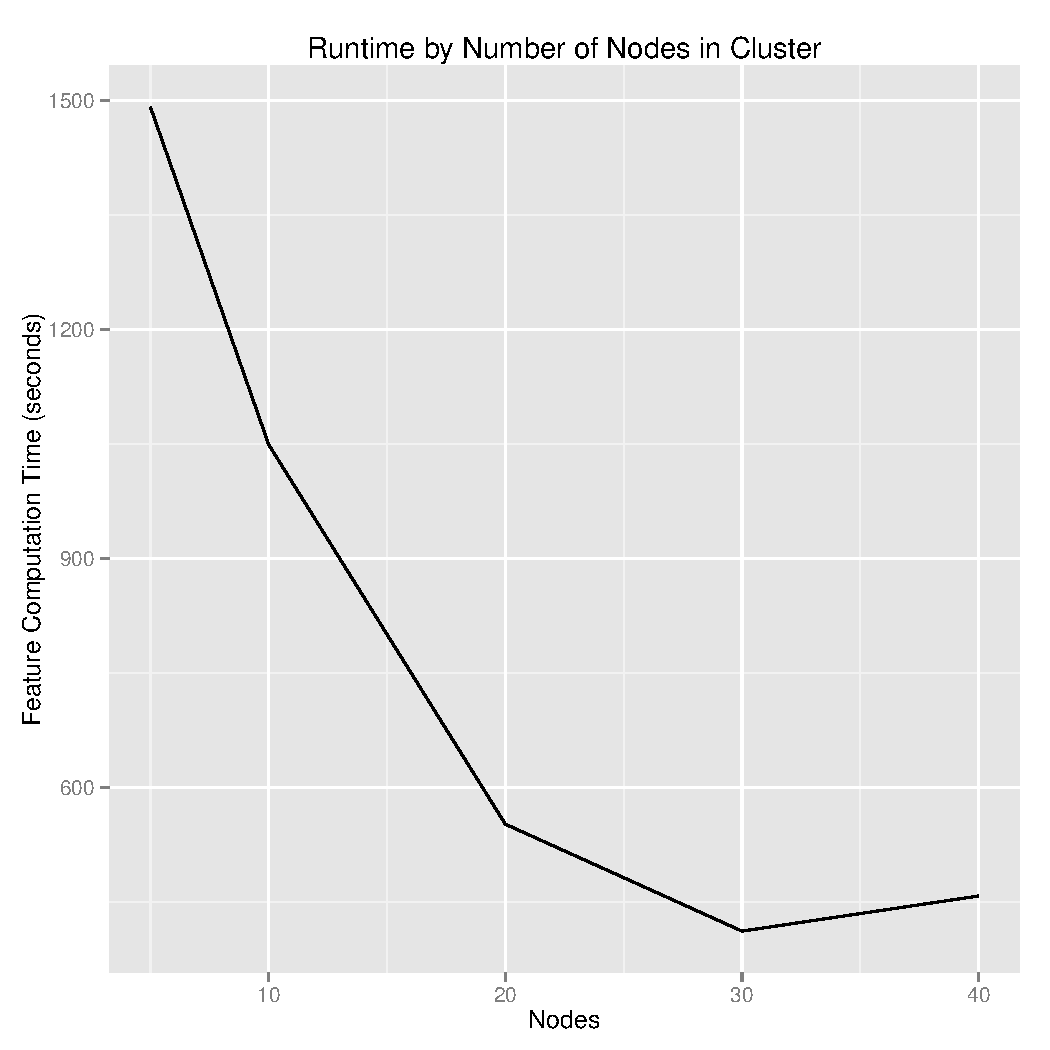
\includegraphics[width=.8\textwidth]{/Users/cwhelan/Documents/svpipeline/figures/runtimeByNodes.pdf}
\caption{Scalability of the Cloudbreak algorithm. Runtime of the Cloudbreak feature generation job for the simulated Chromosome 2 data is shown on Hadoop clusters consisting of varying numbers of compute nodes. Clusters were created in the Amazon Elastic Compute Cloud.}
\label{scalability}
\end{figure}

Choosing the correct operating point or threshold to set on the output of an SV calling algorithm can be difficult when operating on a new data set. The use of simulated data and ROC curves allows for some investigation of the performance characteristics of algorithms at varying levels. First, we characterized the predictions made by each algorithm at the operating point which gives them maximum sensitivity. For Cloudbreak we chose an operating point at which marginal improvements in sensitivity became very low. The results for both deletion and insertion predictions are summarized in Table~\ref{chr2DeletionAndInsertionPredsMaxSensitivity}. MoDIL and Cloudbreak exhibited the greatest recall for deletions. Cloudbreak has high precision and recall for deletions at this threshold, and discovers many more small deletions. For insertions, Cloudbreak has the highest recall, although recall is low for all four approaches. Cloudbreak again identifies the most small variants. Pindel is the only tool which can consistently identify large insertions, as insertions larger than the library insert size do not produce mapping signatures detectable by read-pair mapping. 

We also used the ROC curves to attempt to characterize the predictions made by each algorithm when a low false discovery rate is required. Table~\ref{chr2DeletionPredsFDR10} shows the total number of simulated deletions found by each tool when choosing a threshold that gives an FDR closest to 10\% based on the ROC curve. At this more stringent threshold, Cloudbreak identifies more deletions in every size category than any other tool. Performance on insertions never reached an FDR of 10\% for any threshold, so insertion predictions are not included in this table. \todo{We also examined Cloudbreak's ability to detect events in repetitive regions of the genome, and found that it was similar to the other methods tested (Tables~\ref{deletionRepmaskpreds} and~\ref{insertionRepmaskpreds}).}

\begin{table}
\begin{center}
\begin{tabular}{rrrrrr}
 \hline
 & 40-100bp & 101-250bp & 251-500bp & 501-1000bp & $>$ 1000bp \\ 
 Total Number & 224 & 84 & 82 & 31 & 26\\ 
 \hline
 Cloudbreak & \textbf{68} (17) & \textbf{67} (\textbf{10}) & \textbf{56} (\textbf{5}) & \textbf{11} (\textbf{3}) & \textbf{15} (\textbf{0}) \\ 
 BreakDancer & 52 (8) & 49 (2) & 49 (0) & 7 (0) & 14 (\textbf{0}) \\ 
 GASVPro  & 35 (2) & 26 (0) & 26 (0) & 2 (0) & 6 (\textbf{0}) \\ 
 DELLY-RP  & 22 (1) & 56 (1) & 40 (0) & 8 (0) & 12 (\textbf{0}) \\ 
 DELLY-SR  & 0 (0) & 2 (0) & 28 (0) & 2 (0) & 10 (\textbf{0}) \\ 
 Pindel  & 60 (\textbf{32}) & 16 (0) & 41 (2) & 1 (0) & 12 (\textbf{0})\\ 
 \hline
\end{tabular}
\end{center}
\caption{The number of simulated deletions in the 30X diploid chromosome 2 with Venter indels found by each tool at a 10\% FDR, as well as the number of those deletions that were discovered exclusively by each tool (in parentheses). The total number of deletions in each size class in the true set of deletions is shown in the second row of the header.}
\label{chr2DeletionPredsFDR10}
\end{table}

\begin{table}
\begin{center}
\begin{tabular}{rrr|rr}
 & \multicolumn{2}{c}{Simulated Data} & \multicolumn{2}{c}{NA18507} \\
\hline
 &  Non-repeat & Repeat  &  Non-repeat & Repeat \\ 
 Total Number & 120 & 327 & 562 & 8059 \\ 
  \hline
  Cloudbreak  & \textbf{37} (\textbf{10}) & \textbf{180} (\textbf{25}) & \textbf{300} (\textbf{85}) & \textbf{1166} (\textbf{270}) \\ 
  Breakdancer & 29 (7) & 142 (3) & 192 (11) & 868 (21) \\
  GASVPro     & 16 (1) & 79 (1) & 79 (7) & 330 (16) \\
  DELLY-RP       & 21 (1) & 117 (1) & 152 (6) & 712 (5) \\
  DELLY-SR       & 0 (0) & 42 (0) & 27 (0) & 391 (0) \\
  Pindel      & 18 (9) & 112 (\textbf{25}) & 109 (2) & 536 (7) \\ 
   \hline
\end{tabular}
\end{center}
\caption{Detected deletions on the simulated and NA18507 data sets identified by each tool, broken down by whether the deletion overlaps with a RepeatMasker-annotated element. For both data sets we used the thresholds derived from finding the 10\% FDR level in the simulated data set. The proportion of deletions that overlap repetitive elements discovered by Cloudbreak is similar to that of the other methods.}
\label{deletionRepmaskpreds}
\end{table}


\begin{table}
\begin{center}
\begin{tabular}{rrr|rr}
 & \multicolumn{2}{c}{Simulated Data} & \multicolumn{2}{c}{NA18507} \\
\hline
 &  Non-repeat & Repeat  &  Non-repeat & Repeat \\ 
 Total Number & 133 & 270 & 341 & 355 \\ 
  \hline
  Cloudbreak  & \textbf{32} (11) & \textbf{91} (\textbf{47}) & \textbf{169} (\textbf{61}) & \textbf{148} (\textbf{68}) \\ 
  Breakdancer & 17 (5) & 22 (6) & 82 (7) & 44 (9) \\
  Pindel      & 25 (\textbf{16}) & 54 (30) & 84 (35) & 82 (24) \\ 
  MoDIL      & 5 (0) & 16 (3) & NA & NA \\ 
   \hline
\end{tabular}
\end{center}
\caption{Detected insertions in the simulated and NA18507 data sets identified by each tool, broken down by whether the insertion occurs in a RepeatMasker-annotated element. The maximum sensitivity cutoffs were used for both data sets. The proportion of insertions in repetitive elements discovered by Cloudbreak is similar to that of the other methods.}
\label{insertionRepmaskpreds}
\end{table}


It should be noted that the methods tested here vary in their breakpoint resolution: SR methods have higher resolution than RP methods. Cloudbreak has the lowest resolution of any of the RP tools tested (Figure~\ref{breakpoint_resolution}).\todo{Cloudbreak looses resolution because...} We strive however to increase sensitivity and specificity to actual variants in the hopes that such calls could still be useful even if their resolution is limited. This seems reasonable to us, especially given the possibility of pipelines in which RP calls are validated \emph{in silico} by local assembly methods or split-read methods.

\begin{figure}
\centering
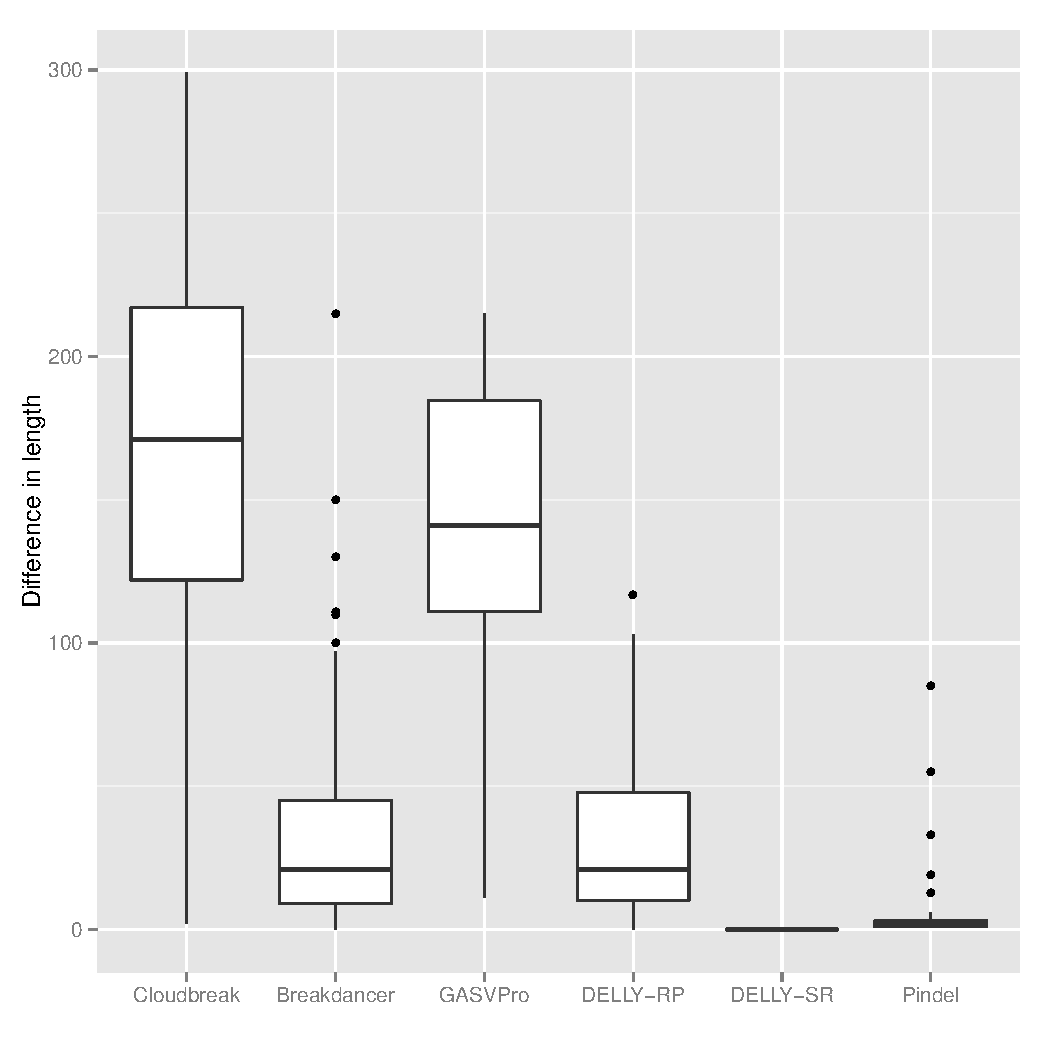
\includegraphics[width=.8\textwidth]{/Users/cwhelan/Documents/svpipeline/figures/breakpoint_resolution.pdf}
\caption{Breakpoint resolution for each tool for deletions on the Chromosome 2 simulated data. For each correctly predicted deletion, we calculated the difference in length between the true deletion and the prediction.}
\label{breakpoint_resolution}
\end{figure}

\begin{table}
\begin{center}
\resizebox{\textwidth}{!}{
\begin{tabular}{r|rrr|rrrrr}
 \cline{2-9}
 &      & Prec. & Recall & 40-100bp & 101-250bp & 251-500bp & 501-1000bp & $>$ 1000bp \\ 
\hline
\multirow{7}{*}{\begin{sideways}Deletions\end{sideways}} & Total Number &   &   & 224 & 84 & 82 & 31 & 26\\ 
 \hline
\cline{2-9}
& Cloudbreak & 0.638 & \textbf{0.678} & \textbf{153} (9) & 61 (0) & 62 (0) & 12 (0) & 15 (0) \\ 
& BreakDancer & 0.356 & 0.49 & 89 (0) & 54 (0) & 53 (0) & 8 (0) & 15 (0) \\ 
& GASVPro  & 0.146 & 0.432 & 83 (2) & 32 (0) & 55 (0) & 8 (0) & 15 (0) \\ 
& DELLY-RP   & 0.457 & 0.613 & 114 (3) & \textbf{68} (0) & \textbf{66} (0) & 9 (1) & 17 (0) \\ 
& DELLY-SR   & \textbf{0.679} & 0.166 & 0 (0) & 3 (0) & 49 (0) & 6 (0) & 16 (0) \\ 
& Pindel   & 0.462 & 0.421 & 96 (\textbf{11}) & 24 (0) & 48 (0) & 5 (0) & 15 (0)\\ 
& MoDIL   & 0.132 & 0.66 & 123 (6) & 66 (\textbf{3}) & \textbf{66} (\textbf{11}) & \textbf{17} (\textbf{7}) & \textbf{23} (\textbf{8})\\ 
 \hline
\multirow{5}{*}{\begin{sideways}Insertions\end{sideways}} & Total Number &   &   & 199 & 83 & 79 & 21 & 21\\ 
\cline{2-9}
& Cloudbreak &0.451 & \textbf{0.305} & \textbf{79} (\textbf{32}) & \textbf{32} (\textbf{18}) & \textbf{11} (8) & 1 (0) & 0 (0) \\ 
& BreakDancer & 0.262 & 0.0968 & 23 (5) & 14 (5) & 2 (1) & 0 (0) & 0 (0) \\ 
& Pindel   & \textbf{0.572} & 0.196 & 52 (25) & 5 (1) & 10 (\textbf{9}) & \textbf{3} (\textbf{2}) & \textbf{9} (\textbf{9})\\ 
& MoDIL   & 0.186 & 0.0521 & 14 (1) & 4 (0) & 1 (0) & 2 (\textbf{2}) & 0 (0)\\ 
\hline
\end{tabular}}
\end{center}
\caption{The number of simulated deletions and insertions in the 30X diploid chromosome 2 with Venter indels found by each tool at maximum sensitivity, as well as the number of those variants that were discovered exclusively by each tool (in parentheses). The total number of variants in each size class in the true set of deletions and insertions is shown in the first row of each section.}
\label{chr2DeletionAndInsertionPredsMaxSensitivity}
\end{table}

\subsection{Tests with Biological Data}

We downloaded a data set of reads taken from a DNA sample of Yoruban individual NA18507, experiment ERX009609 from the Sequence Read Archive. This sample was sequenced on the Illumina Genome Analyzer II platform with 100bp paired end reads and a mean fragment size (minus adapters) of 300bp, with a standard deviation of 15bp, to a depth of approximately 37X coverage.

To create a gold standard set of insertions and deletions to test against, we pooled annotated variants discovered by three previous studies on the same sample. These included data from the Human Genome Structural Variation Project reported by~\cite{Kidd:2008p926}, a survey of small indels conducted by~\cite{Mills:2011fi}, and insertions and deletions from the merged call set of the phase 1 release of the 1000 Genomes Project~\cite{GenomesProjectConsortium:2012co} which were genotyped as present in NA18507. We merged any overlapping calls of the same type into the region spanned by their unions. It should be noted that the 1000 Genomes call set was partially produced using DELLY and BreakDancer, and therefore those calls are ones that those tools are sensitive to, biasing this test in their favor. We were unable to run MoDIL on the whole-genome data set due to the estimated runtime and storage requirements.

\begin{figure}
\centering
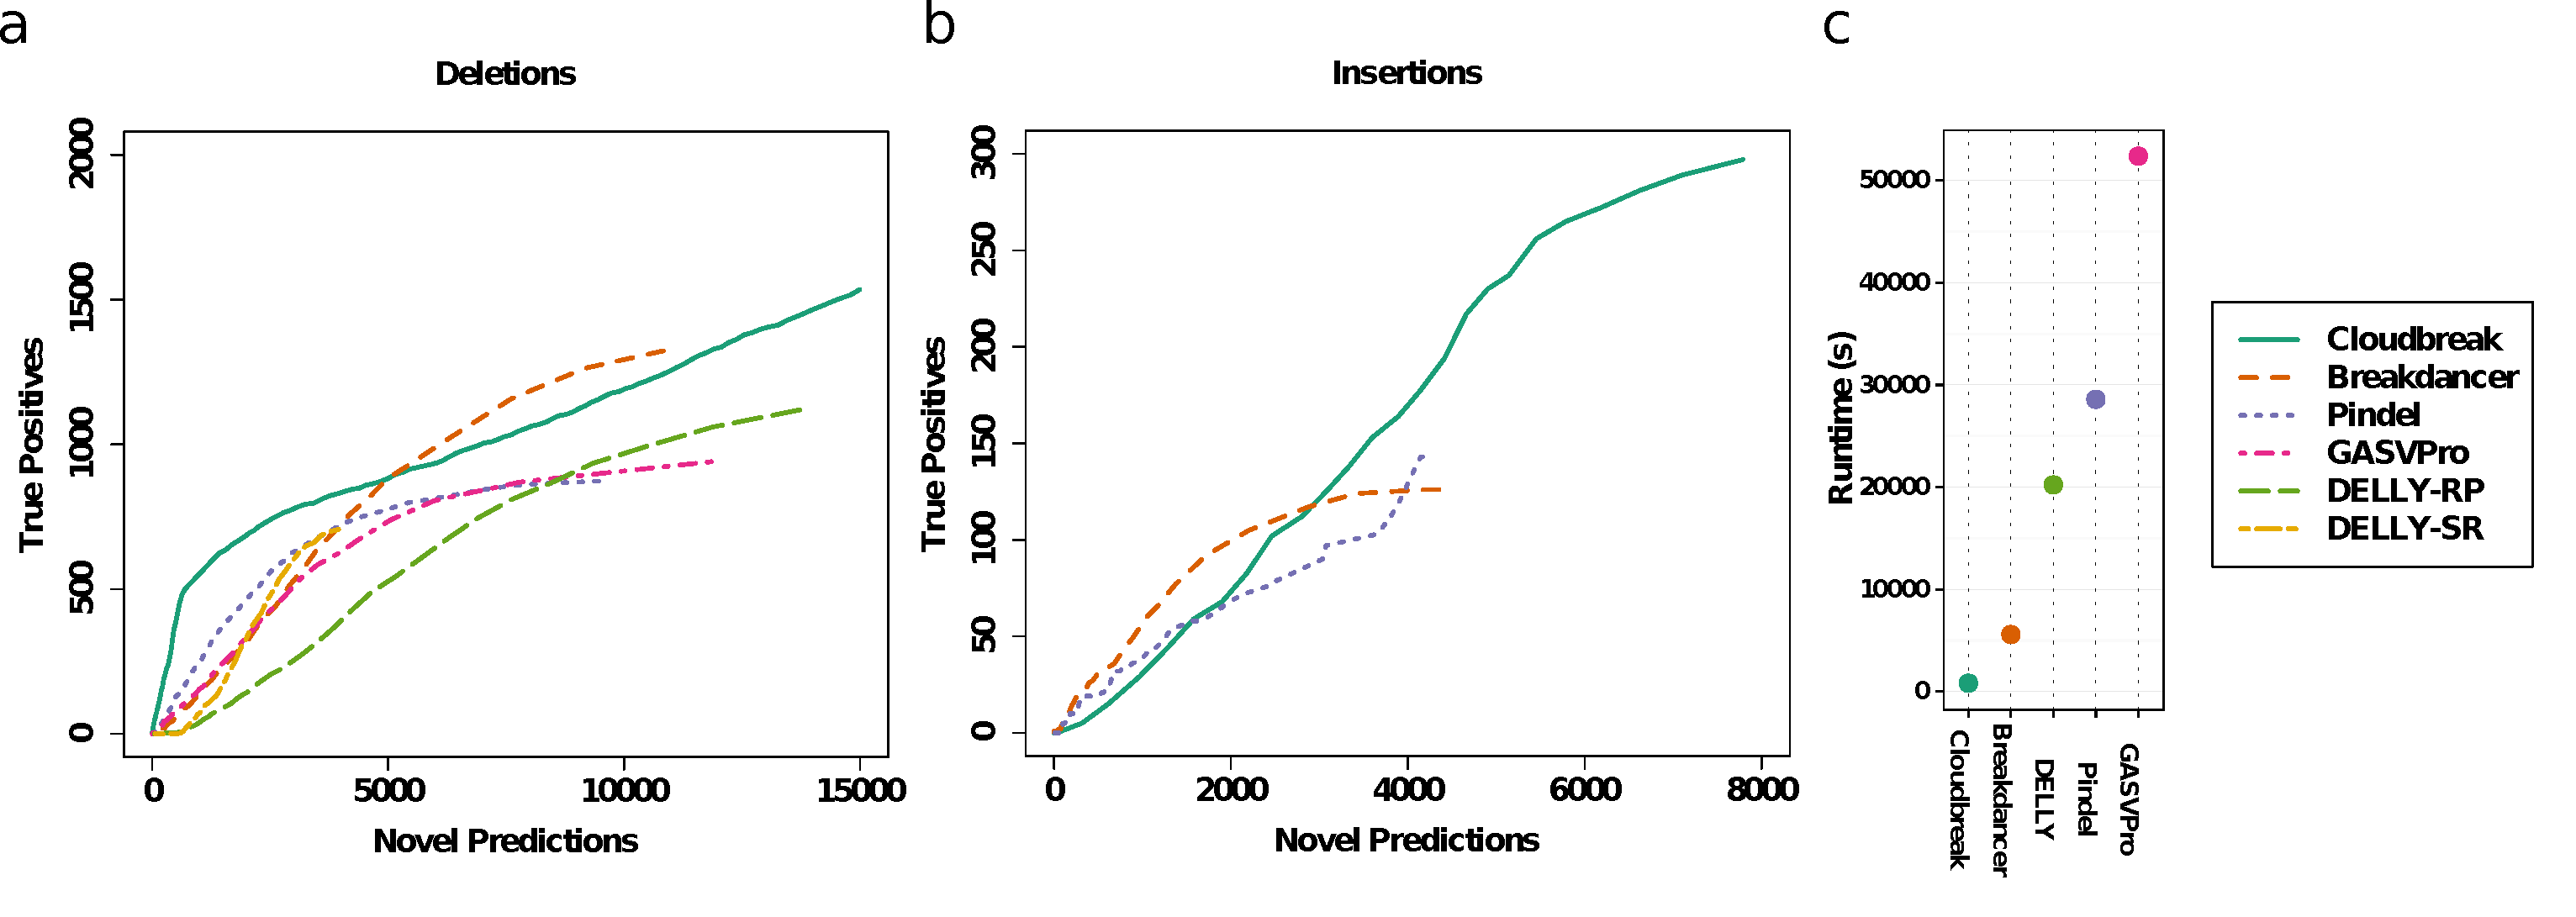
\includegraphics[width=1\textwidth]{figures/NA18507_rocs_runtime.pdf}
\caption{Accuracy and performance on the 37X NA18507 sample. (a) ROC curve for deletion prediction performance, tested against the combined gold standard sets of deletions taken from~\cite{Kidd:2008p926},~\cite{Mills:2011fi}, and~\cite{GenomesProjectConsortium:2012co}. (b) ROC curve for insertion prediction performance. (c) Runtimes for each tool, not including alignment time, parallelized when possible \todo{(see Supplementary Material)}. }
\label{NA18507CombinedRoc}
\end{figure}

Figure~\ref{NA18507CombinedRoc} shows the performance of each algorithm on the NA18507 data set when compared against the gold standard set for both deletions and insertions. All algorithms show far less specificity for the gold standard set than they did for the true variants in the single chromosome simulation, although it is difficult to tell how much of the difference is due to the added complexity of real data and a whole genome, and how much is due to missing variants in the gold standard set that are actually present in the sample. For deletions, Cloudbreak is the best performer at the most stringent thresholds, and has the highest or second highest precision at higher sensitivity levels. Cloudbreak has slightly lower accuracy for insertions than other tools, although it can identify the most variants at higher levels of sensitivity. As shown in Table~\ref{runtimes}, Cloudbreak processes the sample in under 15 minutes on our cluster, more than six times as fast as the next fastest program, BreakDancer, even when BreakDancer is run in parallel for each chromosome on different nodes in the cluster.

Given the high number of false positives produced by all tools at maximum sensitivity indicated by the ROC curves, we decided to characterize the predictions made by each tool at more stringent thresholds. We examined the deletion predictions made by each algorithm using the same cutoffs that yielded a 10\% FDR on the simulated chromosome 2 data set, adjusted proportionally for the difference in coverage from 30X to 37X. For insertions, again, we were forced to use the thresholds that gave maximum sensitivity for each tool due to the high observed FDR rates in the simulated data. The precision and recall at these thresholds with respect to the gold standard set, as well as the performance of each algorithm at predicting variants of each size class at those thresholds, is shown in Table~\ref{NA18507DeletionAndInsertionPreds}. For deletions, Cloudbreak has the greatest sensitivity of any tool at these thresholds, identifying the most variants in each size class. Pindel exhibits the highest precision with respect to the gold standard set. For insertions, Pindel again has the highest precision at maximum sensitivity, although according the ROC curve it is possible to choose a threshold for Cloudbreak with higher precision and recall. At maximum sensitivity, Cloudbreak identifies 120 more insertions from the gold standard set than Pindel, giving it by far the highest recall.

\begin{table}
\begin{center}
\resizebox{\textwidth}{!}{
\begin{tabular}{r|rrr|rrrrr}
 \cline{2-9}
& & Prec. & Recall & 40-100bp & 101-250bp & 251-500bp & 501-1000bp & $>$ 1000bp \\ 
\hline
\multirow{6}{*}{\begin{sideways}Deletions\end{sideways}} & Total Number & & & 7,462 & 240 & 232 & 147 & 540 \\
 \hline
\cline{2-9}
& Cloudbreak & 0.0943 & \textbf{0.17} & \textbf{573} (\textbf{277}) & \textbf{176} (\textbf{30}) & \textbf{197} (\textbf{18}) & \textbf{121} (\textbf{6}) & \textbf{399} (\textbf{24}) \\ 
& BreakDancer & 0.137 & 0.123 & 261 (29) & 136 (3) & 178 (0) & 114 (0) & 371 (0) \\ 
& GASVPro & 0.147 & 0.0474 & 120 (21) & 40 (2) & 85 (0) & 36 (0) & 128 (0) \\ 
& DELLY-RP & 0.0931 & 0.1 & 143 (6) & 128 (3) & 167 (1) & 103 (0) & 323 (1) \\ 
& DELLY-SR & 0.153 & 0.0485 & 0 (0) & 26 (0) & 123 (0) & 66 (0) & 203 (0) \\ 
& Pindel & \textbf{0.179} & 0.0748 & 149 (8) & 61 (0) & 149 (0) & 69 (1) & 217 (0) \\ 
\hline
\multirow{4}{*}{\begin{sideways}Insertions\end{sideways}} & Total Number & & & 536 & 114 & 45 & 1 & 0 \\
\cline{2-9}
& Cloudbreak & 0.0323 & \textbf{0.455} & \textbf{265} (\textbf{104}) & \textbf{49} (\textbf{24}) & 3 (1) & 0 (0) & 0 (0) \\ 
& BreakDancer & 0.0281 & 0.181 & 97 (10) & 27 (5) & 2 (1) & 0 (0) & 0 (0) \\ 
& Pindel & \textbf{0.0387} & 0.239 & 144 (45) & 14 (7) & \textbf{7} (\textbf{6}) & \textbf{1} (\textbf{1}) & 0 (0) \\ 
\hline
\end{tabular}}
\end{center}
\caption{The precision and recall with respect to the gold standard set of deletions and insertions for each tool on the NA18507 data, as well as the number of variants found in each size class found. Exclusive predictions are in parentheses. For deletions, the same cutoffs were used as for the simulated data as in Table~\ref{chr2DeletionPredsFDR10}, adjusted for the difference in coverage from 30X to 37X. For insertions, the maximum sensitivity cutoff was used.}
\label{NA18507DeletionAndInsertionPreds}
\end{table}

\subsection{Performance on a Low-Coverage Cancer Data Set}

We also tested Cloudbreak on a sequencing data set obtained from a patient with acute myeloid leukemia (AML). This data set consisted of 76bp paired end reads with a mean insert size of 285bp and standard deviation of 50bp, yielding sequence coverage of 5X and physical coverage of 8X. Using a pipeline consisting of Novoalign, BreakDancer, and a set of custom scripts for filtering and annotating candidate SVs, we had previously identified a set of variants present in this sample and validated several using PCR, including 8 deletions. Cloudbreak was able to identify all 8 of the validated deletions, showing that it is still sensitive to variants even when using lower coverage data sets with a greater variance of insert sizes. The variants identified include deletions in the gene CTDSPL/RBPS3, an AML tumor suppressor~\cite{Zheng:2012kk}, and NBEAL1, a gene up-regulated in some cancers~\cite{Chen:2004jo}. We are currently investigating these deletions to determine their functional impact on this patient. 

\subsection{Genotyping Variants}

Because Cloudbreak explicitly models zygosity in its feature generation algorithm, it can predict the genotypes of identified variants. We tested this on both the simulated and NA18507 data sets. For the NA18507 data set, we considered the deletions from the 1000 Genomes Project, which had been genotyped using the population-scale SV detection algorithm Genome STRiP \cite{Handsaker:2011ki}. Cloudbreak was able to achieve 92.7\% and 95.9\% accuracy in predicting the genotype of the deletions it detected at our 10\% FDR threshold in the simulated and real data sets, respectively. Table~\ref{deletionGenotypeaccuracy} shows confusion matrices for the two samples using this classifier. None of the three input sets that made up the gold standard for NA18507 contained a sufficient number of insertions that met our size threshold and also had genotyping information. Of the 123 insertions detected by Cloudbreak on the simulated data set, 43 were heterozygous. Cloudbreak correctly classified 78 of the 80 homozygous insertions and 31 of the 43 heterozygous insertions, for an overall accuracy of 88.6\%.

\begin{table}
\begin{center}
\begin{tabular}{r|r|rr|rr|}
\multicolumn{2}{c}{}  & \multicolumn{4}{c}{Actual Genotypes} \\
\multicolumn{2}{c}{}  & \multicolumn{2}{c}{Simulated Data} & \multicolumn{2}{c}{NA18507} \\
\cline{3-6}
\multicolumn{2}{c|}{} &  Homozygous & Heterozygous & Homozygous & Heterozygous \\ 
\cline{2-6}
\multirow{2}{*}{\shortstack{Predicted \\ Genotypes}} & Homozygous & 35 & 2 &  96 & 21 \\
 & Heterozygous & 0 & 39 &  2 & 448 \\
\cline{2-6}
\end{tabular}
\end{center}
\caption{Confusion matrices for the predicted genotype of deletions found by Cloudbreak on both the simulated and NA18507 data sets.}
\label{deletionGenotypeaccuracy}
\end{table}

\chapter{Extending Local Feature Based Models of SV Detection in a Discriminative Machine Learning Framework}

In my formulation of a general approach for SV prediction in the MapReduce framework, a crucial phase is the computation of a set of features for each genomic location. In my current implementation of Cloudbreak, these features are the parameters which are estimated by fitting a GMM to the distribution of insert sizes that span that location. However, the nature of these features are purposefully not specified in the algorithmic framework to allow flexibility in the implementation of the framework.

Given a set of arbitrary features that encode information about a set of loci that are connected in a sequence, a natural approach is to apply techniques from machine learning to identify regions of interest in that sequence, rather than the heuristics and noise reduction techniques from signal processing that are currently used in the Cloudbreak implementation. Machine learning techniques have been applied to SV detection in the packages forestSV~\cite{Michaelson:2012fj} and SVM$^2$~\cite{Chiara:2012ey}, and a form of generative modeling is applied to region features in SVMiner~\cite{Hayes:2012ia}. However, none of these tools use machine learning techniques that take into account the sequential nature of the data. 

I propose using features generated by Cloudbreak and a set of representative training data to train a discriminative classifier to label regions of the genome as either normal or affected by an insertion or deletion. In preliminary work conducted with an earlier version of Cloudbreak, I attempted to use linear-chain conditional random fields~\cite{Lafferty:2001:CRF:645530.655813} (CRFs) to label genomic deletions. Although I did not achieve a useful level of performance, I believe that this is still a useful area of investigation. During my preliminary work, I encountered issues relating to class imbalance in the training sets and the inability of CRF training frameworks to handle real-valued feature vectors. I will address these issues by constructing new training sets, engineering new feature sets that the current version of Cloudbreak is now able to construct, and utilizing frameworks that can work with real-valued features, such as Factorie~\cite{mccallum09:factorie}. As an alternative to CRFs, I will also investigate the use of deep learning techniques such as sequential deep belief networks~\cite{andrew2012:sdbn}, which have been used successfully in sequence processing tasks in speech recognition and other domains.

The outcome of this extension will be: the creation of a training, development, and test set, along with a feature generation scheme and description of the model used; an evaluation of the performance gains that can be achieved, with a comparison to other SV detection approaches; and a discussion of the benefits and drawbacks of using such an approach.

\section{SV Detection as a Sequence Labeling Problem}

\section{Features for SV Detection}

\section{Integrating features with Conditional Random Fields}

\section{Improving Cloudbreak Calls with CRF Predictions}

\chapter{Analysis of Breakpoint Features in Evolutionary and Cancer Contexts}

It is important not only to be able to locate genomic breakpoints, but also to understand the genomic contexts in which they are located. This can give insights into the mechanisms of their formation, and to their impact on genome structure and function. As mentioned previously, evolutionary breakpoints that break synteny between species have parallels in the genomic breakpoints that occur within cancer cells: at some point in time SVs created these breakpoints, which were then conserved through evolutionary history. One especially interesting example can be found in the genome of the gibbon, which has many more genomic rearrangements with respect to the other apes than would be expected given their degree of relatedness.

\section{Evolutionary Breakpoints in the Gibbon Genome determined by BACs}

To search for genomic features potentially associated with gibbon chromosomal breakpoints I computed the significance of the overlap between gibbon evolutionary breakpoint regions, which had been identified and mapped to the human genome using bacterial artificial chromosomes (BACs) and array painting, and a set of genomic features of interest using permutation tests~\cite{Capozzi:2012bb}. The purpose of the permutation analysis is to discover the null distribution for the number of overlaps a set of intervals has with a particular feature in the genome. In essence, the test asks: if my intervals were placed in random locations on the genome, what is the probability of seeing the number of overlaps we observed with that features in the actual data? 

To conduct the test, while maintaining the chromosomal assignment and length of break- point regions, we permuted their start coordinates 10,000 times using BEDTools version 2.16.2~\cite{Quinlan:2010km}. Genomic regions annotated as centromeres and telomeres in the ``Gaps'' track of the hg19 build were excluded from possible random placements of the regions. Locations of the features were held constant. We then compared the number of features that overlapped a breakpoint region to the observed distribution of results among the randomly permuted regions, and used the quantile of the real observed value in that distribution as an estimate of the P-value of observing a value equal to or greater than the real observation. In order to be able to conduct a large number of permutations to determine a true background distribution for each feature, I have created a pipeline for distributing computation across a compute cluster using the grid management system HTCondor.

The analysis was performed on the human hg19 assembly. The features examined were genes, human segmental duplications, and some repeat families (Alu, LINE, ERV, and SVA). We also investigated the associations between breakpoint regions and chromatin structure by testing the overlap with open chromatin regions in human embryonic stem cells reported by the ENCODE consortium~\cite{ENCODEProjectConsortium:2011iz}. We found a significant enrichment for genes (Bonferroni adjusted P-value = 0.0287), human segmental duplications (P = 0.0366), Alu (P < 0.0001), and SVA (P = 0.0008) (Fig.~\ref{gibbon_bac_permutations}A). We did not find significant enrichment for LINE and ERV repeats, nor for the ENCODE open chromatin regions. Systematically shifting the location of breakpoint regions by increments of 10 kb up- and downstream of their actual location, up to a maximum of 1 MB, shows that the locations of the breakpoint regions gives the greatest or close to the greatest number of overlaps with the four significantly overlapping features (genes, segmental duplications, Alu, and SVA) in the local genomic neighborhood (Fig.~\ref{gibbon_bac_permutations}B).

\begin{figure}
\centering
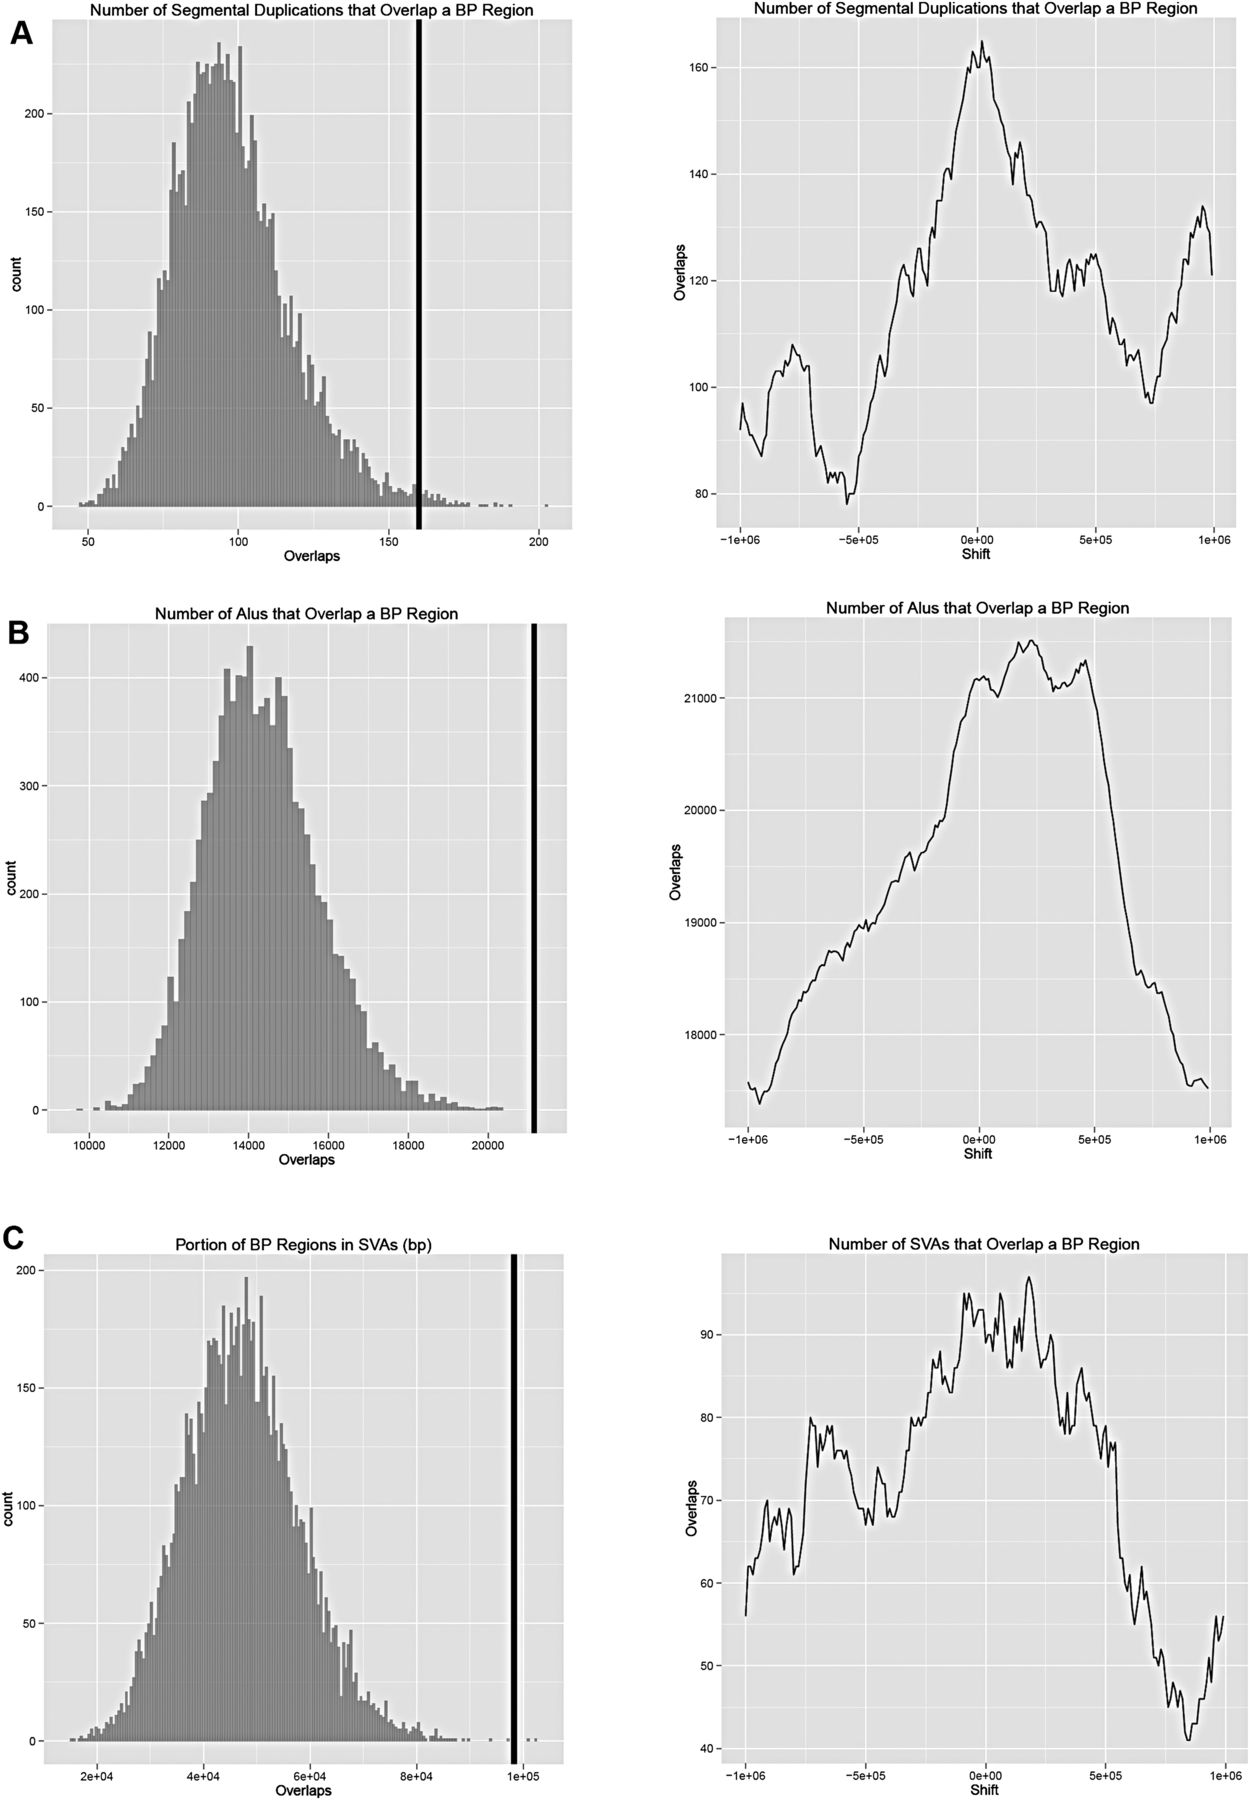
\includegraphics{figures/gibbon_bac_permutations.jpg}
\caption{Enrichment of genomic features in breakpoint regions. Permutation tests were used to assess the overlap between the gibbon breakpoints and genomic features. (A) Segmental duplications; (B) Alu elements; and (C) SVA elements. The black vertical line indicates the observed value for the breakpoints identified in the study. In all three cases it is evident that the genomic features have a higher overlap with the breakpoints than one could expect by chance.}
\label{gibbon_bac_permutations}

\end{figure}

\section{Continuing Analysis of Genomic Breakpoints from Cancer and Evolution}

Continuing the work I have already done in analyzing the evolutionary breakpoints mapped with the gibbon BAC clones, I am working with the International Consortium for Sequencing and Annotation of the gibbon genome to analyze the additional breakpoints discovered through the assembly of the gibbon reference genome. To do so, I am conducting additional association tests with a variety of features. One of these features is a set of binding sites of the evolutionarily conserved binding factor CTCF, which I have identified through the analysis of chromatin immunoprecipitation followed by sequencing (ChIP-seq) data. CTCF has recently been shown to be associated with the three-dimensional structure of DNA and chromatin in the cell~\cite{Dixon:2012gc}, and therefore may have important associations with genomic DNA breakpoints and structural variations.

I am also helping to analyze the breakpoints from a set of over forty mesenchymal tumor samples in which genomic rearrangements have created ring-shaped chromosomes. The breakpoints that cause these chromosomal rearrangements cluster into several frequently broken areas. I am currently working on analyzing these breakpoint regions using my permutation analysis pipeline in order to determine genomic features that may be significantly associated with these breakpoints, including repeat elements, open chromatin sites and other data from ENCODE, and binding motifs for enzymes known to be involved with breakpoint formation.

As part of these analyses I will also explore alternative testing strategies including hypergeometric testing~\cite{Sandve:2013ip} and spatial correlation testing~\cite{Favorov:2012dy}.

\chapter{Future Work}

There are many possible extensions that could be made to enhance Cloudbreak's effectiveness as a general SV analysis tool for high-throughput sequencing data. However, implementing all of them is outside of the scope of this thesis, which aims to demonstrate the general effectiveness of a distributed computing approach to SV detection. These other extensions include:

\begin{itemize}
 \item Detection of additional SV types such as longer deletions, inversions, and translocations. While these would be useful and necessary additions to a complete variant detection pipeline, I believe that by showing the applicability of MapReduce to two classes of variants (short-to-midsize deletions, and short insertions), Cloudbreak will create a base from which to implement many additional SV detection algorithms in the future.
 \item Addition of a local assembly step to increase breakpoint resolution and validate SV candidates. Cloudbreak's breakpoint resolution is less than that of many other RP and SR algorithms. One approach to improving breakpoint resolution, and providing additional validation of predicted results, is to attempt to conduct a \emph{de novo} assembly of the reads that mapped near the breakpoints and their pairs. If effectively implemented, this would be a very useful addition to any SV detection algorithm. However, the implementation of such an approach in a distributed setting would likely be embarrassingly parallel, with multiple instantiations of a self-contained assembly algorithm run on different compute nodes. Therefore, it would not necessarily add to the demonstration of the effectiveness of the MapReduce framework to this domain.
 \item Incorporation of split-read signals into the Cloudbreak implementation. As sequencing technology improves, read lengths will continue to lengthen, making split-read mapping a more effective strategy for SV detection. Therefore, we have considered adding a split-read mapping algorithm to Cloudbreak as well. However, as with local assembly discussed above, non-distributed split-read aligners run in parallel for different subsets of the input reads would likely be just as effective. In addition, I believe that my formulation of SV detection based on genomic features could be extended to include a new set of features created by executing split-read mappers, especially in the context of the machine-learning approaches described above.
\end{itemize}

In summary, rather than providing a broad but shallow implementation of many possible application features, I believe that the demonstration of a system that leverages cluster and cloud computing to achieve state-of-the-art accuracy and runtime performance on a subset of the SV detection problem will provide a higher impact to the genomic sequencing research community.

% The library likes numbers rather than the `alpha' style.
\bibliographystyle{acm}
% Single space the bibliography to save space.
\begin{singlespace}
\bibliography{thesis}
\end{singlespace}
%\printbibliography

% The appendices are optional, but they must follow the references.
%\appendix

% This section (the final one) contains a biographical note.
%
%\vita
%This section contains a biographical note.
%The following information (in essay form) should be contained in this section:
%place of birth; date of birth; schools attended; degrees awarded; areas of
%special interest; relevant profession experience; awards and honors; list
%of publications.

\end{document}
